\documentclass[12pt,a4paper]{report}

% =========================================================================
% GÓI THƯ VIỆN & CẤU HÌNH CƠ BẢN (XELATEX COMPATIBLE)
% =========================================================================
\usepackage{fontspec}
\setmainfont{Times New Roman}

\usepackage[top=2.5cm, bottom=2.5cm, left=3.0cm, right=2.0cm]{geometry}
\usepackage{amsmath, amsfonts, amssymb}
\usepackage{graphicx}
\usepackage{booktabs}
\usepackage{tabularx}
\usepackage{multirow}
\usepackage{array}
\usepackage{float}
\usepackage{xcolor}
\usepackage{tikz}
\usetikzlibrary{calc, shapes.geometric, arrows.meta, positioning}
\usepackage{hyperref}
\usepackage{fancyhdr}
\usepackage{titlesec}
\usepackage{caption}
\usepackage{subcaption}
\usepackage{enumitem}
\usepackage{listings}

% Cấu hình Hyperref
\hypersetup{
    colorlinks=true,
    linkcolor=blue!80!black,
    citecolor=green!60!black,
    urlcolor=blue!70!black,
    pdftitle={Báo Cáo Assignment 01 - Phát Triển Hệ Thống Thông Minh},
    pdfauthor={Phạm Văn Tư - B23DCCN879}
}

% Cấu hình Code Listing
\definecolor{codegreen}{rgb}{0,0.6,0}
\definecolor{codegray}{rgb}{0.5,0.5,0.5}
\definecolor{codepurple}{rgb}{0.58,0,0.82}
\definecolor{backcolour}{rgb}{0.96,0.97,0.98}

\lstdefinestyle{mystyle}{
    backgroundcolor=\color{backcolour},   
    commentstyle=\color{codegreen},
    keywordstyle=\color{blue!80!black}\bfseries,
    numberstyle=\tiny\color{codegray},
    stringstyle=\color{codepurple},
    basicstyle=\ttfamily\footnotesize,
    breakatwhitespace=false,         
    breaklines=true,                 
    captionpos=b,                    
    keepspaces=true,                 
    numbers=left,                    
    numbersep=5pt,                  
    showspaces=false,                
    showstringspaces=false,
    showtabs=false,                  
    tabsize=2,
    frame=single,
    rulecolor=\color{black!20}
}
\lstset{style=mystyle}

% Định dạng tiêu đề chương, mục
\titleformat{\chapter}[display]
  {\normalfont\bfseries\color{blue!80!black}}
  {\filleft\Large\bfseries\chaptertitlename\ \thechapter}
  {1ex}
  {\titlerule\vspace{1ex}\filright\LARGE}
  [\vspace{1ex}\titlerule]

\titleformat{\section}
  {\normalfont\Large\bfseries\color{blue!70!black}}
  {\thesection}{1em}{}

\titleformat{\subsection}
  {\normalfont\large\bfseries\color{black!85}}
  {\thesubsection}{1em}{}

% Header & Footer
\pagestyle{fancy}
\fancyhf{}
\fancyhead[R]{\small\itshape Báo cáo Assignment 01: From Data Representation to a First Intelligent System}
\fancyfoot[C]{\thepage}
\renewcommand{\headrulewidth}{0.4pt}
\renewcommand{\footrulewidth}{0.4pt}

% =========================================================================
% BẮT ĐẦU TÀI LIỆU
% =========================================================================
\begin{document}

% -------------------------------------------------------------------------
% TRANG BÌA CHUẨN PTIT (ĐỒNG BỘ 100% VỚI TEMPLATE DOCX VÀ HÌNH MẪU)
% -------------------------------------------------------------------------
\begin{titlepage}
\begin{tikzpicture}[remember picture, overlay]
    % Khung viền họa tiết hoa văn cổ điển có padding cách mép giấy 1.0cm
    \node[anchor=center] at (current page.center) {
        
\includegraphics[width=\dimexpr\paperwidth-2.0cm\relax, height=\dimexpr\paperheight-2.0cm\relax]{images/ptit_cover_border.jpeg}
    };
\end{tikzpicture}

\begin{center}
    \vspace*{-0.2cm}
    {\fontsize{14.5pt}{19pt}\selectfont \textbf{HỌC VIỆN CÔNG NGHỆ BƯU CHÍNH VIỄN THÔNG}}\\[0.3cm]
    {\fontsize{14.5pt}{19pt}\selectfont \textbf{KHOA CÔNG NGHỆ THÔNG TIN 1}}\\[0.3cm]
    {\fontsize{14.5pt}{19pt}\selectfont \textbf{HỌC PHẦN PHÁT TRIỂN CÁC HỆ THỐNG THÔNG MINH}}\\[1.1cm]
    
    % Logo PTIT chuẩn
    
\includegraphics[width=4.5cm]{images/ptit_logo.png}\\[1.3cm]
    
    {\fontsize{18pt}{22pt}\selectfont \textbf{ASSIGNMENT 01}}\\[0.4cm]
    {\fontsize{13pt}{17pt}\selectfont \textbf{ĐỀ TÀI: XÂY DỰNG HỆ THỐNG CHẨN ĐOÁN TIỂU ĐƯỜNG \&}}\\[0.15cm]
    {\fontsize{13pt}{17pt}\selectfont \textbf{ĐỊNH GIÁ BẤT ĐỘNG SẢN TÍCH HỢP ĐỒ THỊ TRI THỨC}}\\[1.1cm]
\end{center}

\begin{flushleft}
    \hspace{2.8cm}
    \begin{tabular}{ll}
        \textbf{Lớp:} & D23CTPM01 \\[0.3cm]
        \textbf{Họ và tên:} & Phạm Văn Tư \\[0.3cm]
        \textbf{Mã sinh viên:} & B23DCCN879 \\[0.3cm]
        \textbf{Giảng viên hướng dẫn:} & PGS.TS Trần Đình Quế \\[0.3cm]
        \textbf{Học kỳ:} & Học kỳ 1 năm học 2026 – 2027
    \end{tabular}
\end{flushleft}

\vfill
\begin{center}
    {\fontsize{12pt}{15pt}\selectfont \textbf{Hà Nội, 2026}}\\[0.4cm]
\end{center}
\end{titlepage}

% -------------------------------------------------------------------------
% MỤC LỤC & DANH MỤC HÌNH ẢNH
% -------------------------------------------------------------------------
\pagenumbering{roman}
\tableofcontents
\newpage
\listoffigures
\listoftables
\newpage
\pagenumbering{arabic}

% =========================================================================
% LỜI MỞ ĐẦU
% =========================================================================
\chapter*{Lời Mở Đầu}
\addcontentsline{toc}{chapter}{Lời Mở Đầu}

Trong bối cảnh dữ liệu số bùng nổ, việc nghiên cứu và phát triển các \textbf{Hệ thống Thông minh (Intelligent Systems)} đã trở thành trọng tâm cốt lõi của ngành Công nghệ Thông tin. Một hệ thống thông minh thực thụ không chỉ dừng lại ở việc áp dụng các mô hình máy học để dự đoán con số xác suất, mà đòi hỏi một quy trình kỹ thuật hoàn chỉnh: từ thấu hiểu bài toán thực tế, lựa chọn phương pháp biểu diễn dữ liệu tính toán, kiểm soát thực nghiệm khoa học, tích hợp tri thức miền (Domain Knowledge) đến triển khai thành ứng dụng thực tiễn phục vụ người dùng.

Báo cáo trình bày toàn bộ quá trình nghiên cứu, thiết kế kiến trúc, hiện thực hóa mã nguồn và đánh giá thực nghiệm cho hai hệ thống thông minh tiêu biểu:
\begin{enumerate}[leftmargin=2em]
    \item \textbf{Hệ thống Chẩn đoán Nguy cơ Tiểu đường (AI Diabetes Diagnostic System):} Giải quyết bài toán phân loại nhị phân trên dữ liệu y sinh, ứng dụng kỹ thuật tiền xử lý dữ liệu lâm sàng, so sánh đối đầu 5 mô hình học máy, kiểm chuẩn độ bền vững trên tập dữ liệu độc lập gồm 2,000 bệnh nhân Bệnh viện Frankfurt (Đức) và tích hợp Đồ thị Tri thức Dược phẩm FPT Long Châu.
    \item \textbf{Hệ thống Định giá Bất động sản Việt Nam (Vietnam Real Estate Valuation System):} Giải quyết bài toán hồi quy đa biến trên dữ liệu thị trường nhà đất quy mô lớn, xử lý dữ liệu chuỗi địa chỉ không gian, khảo sát 5 mô hình hồi quy phi tuyến, đánh giá khả năng tổng quát hóa ngoài phân phối (Out-of-Distribution Generalization) trên tập dữ liệu kiểm chuẩn độc lập gồm 2,000 tin đăng bất động sản tại các thị trường đô thị mở rộng (Đà Nẵng, Hải Phòng, Bình Dương, Hưng Yên) và tích hợp Đồ thị Tri thức Tiện ích Đô thị \& Gói vay Ngân hàng.
\end{enumerate}

Toàn bộ hệ thống được đóng gói thành các vi dịch vụ REST API hiệu năng cao trên nền tảng FastAPI và triển khai giao diện Web Responsive hiện đại, tự động thích ứng tối ưu trên mọi kích thước màn hình từ Desktop, Laptop, Máy tính bảng đến Điện thoại thông minh.

\newpage

% =========================================================================
% CHƯƠNG 1: CƠ SỞ LÝ THUYẾT VÀ NGUYÊN LÝ HỆ THỐNG THÔNG MINH
% =========================================================================
\chapter{Cơ sở Lý thuyết \& Nguyên lý Hệ thống Thông minh}

\section{Khái niệm về Tính thông minh và Hệ thống thông minh}

\subsection{Tính thông minh thao tác (Operational Intelligence) trong Học máy}
Trong khoa học máy tính và trí tuệ nhân tạo, tính thông minh của một hệ thống máy học truyền thống được xác định thông qua năng lực thực thi tác vụ:
\begin{equation}
\text{Intelligence} = \text{Learning from Examples} + \text{Generalization} + \text{Prediction}
\end{equation}

Một hệ thống được xem là thể hiện hành vi thông minh khi thỏa mãn chu trình khép kín:
\begin{enumerate}[leftmargin=1.5em]
    \item \textbf{Thu nhận tín hiệu (Perception):} Tiếp nhận các quan sát, số liệu đo lường từ môi trường thực tế.
    \item \textbf{Biểu diễn tính toán (Representation):} Ánh xạ các quan sát sang cấu trúc toán học trong không gian vector số thực $\mathbb{R}^d$.
    \item \textbf{Tự động học quy luật (Learning):} Trích xuất mối liên hệ tiềm ẩn giữa thuộc tính đầu vào và nhãn mục tiêu thông qua tối ưu hóa hàm mục tiêu.
    \item \textbf{Năng lực tổng quát hóa (Generalization):} Suy luận chính xác trên những quan sát hoàn toàn mới chưa từng xuất hiện trong tập huấn luyện.
    \item \textbf{Ra quyết định và Hành động (Decision \& Action):} Đưa ra kết luận hỗ trợ chuyên gia (bác sĩ, nhà thẩm định) hoặc kích hoạt quy trình tự động.
\end{enumerate}

\subsection{Dòng chảy thông tin trong Hệ thống Thông minh}
Kiến trúc luân chuyển thông tin từ thế giới thực đến quyết định suy luận được mô tả như Hình \ref{fig:ml_flow}.

\begin{figure}[H]
\centering
\begin{tikzpicture}[
    block/.style={rectangle, draw=blue!80!black, fill=blue!6, thick, rounded corners=4pt, minimum width=2.2cm, minimum height=1.1cm, align=center, font=\footnotesize\bfseries},
    arrow/.style={draw=blue!80!black, thick, -{Latex[length=2.5mm, width=1.5mm]}}
]
    \node [block] (env) at (0, 0) {Thế giới\\thực tế};
    \node [block] (data) at (3.2, 0) {Dữ liệu\\thu thập};
    \node [block] (rep) at (6.6, 0) {Vector\\đặc trưng $\mathbf{x} \in \mathbb{R}^d$};
    \node [block] (ml) at (10.0, 0) {Mô hình\\học máy $f_\theta$};
    \node [block] (pred) at (13.2, 0) {Quyết định\\dự đoán $\hat{y}$};
    
    \draw [arrow] (env) -- (data);
    \draw [arrow] (data) -- (rep);
    \draw [arrow] (rep) -- (ml);
    \draw [arrow] (ml) -- (pred);
\end{tikzpicture}
\caption{Dòng chảy Biểu diễn và Xử lý Thông tin trong Hệ thống Thông minh}
\label{fig:ml_flow}
\end{figure}

\section{Bản chất của Biểu diễn Dữ liệu (Data Representation) trong AI}

\subsection{Nguyên lý Hình học của Không gian Vector Đặc trưng ($\mathbb{R}^d$)}
Một nguyên lý nền tảng và bất biến trong trí tuệ nhân tạo là: \textit{Các thuật toán học máy không tiếp xúc trực tiếp với thế giới thực, mà chỉ vận hành trên một không gian biểu diễn tính toán của các thuộc tính được chọn lọc.} 

Mỗi thực thể trong thế giới thực (một bệnh nhân khám bệnh hoặc một căn nhà trên thị trường) được ánh xạ thành một điểm dữ liệu trong không gian vector Euclid $d$ chiều:
\begin{equation}
\mathbf{x}_i = [x_{i1}, x_{i2}, \dots, x_{id}]^T \in \mathbb{R}^d, \quad i = 1, \dots, N
\end{equation}

Tập dữ liệu huấn luyện có giám sát được cấu trúc thành ma trận dữ liệu và vector nhãn mục tiêu:
\begin{equation}
\mathcal{D} = \{(\mathbf{x}_i, y_i)\}_{i=1}^N \iff \mathbf{X} \in \mathbb{R}^{N \times d}, \quad \mathbf{y} \in \mathcal{Y}^N
\end{equation}

\textbf{Mối liên hệ hình học và hiệu năng mô hình:} Hình học của không gian đặc trưng quyết định hoàn toàn độ phức tạp của bài toán học máy. Nếu các lớp dữ liệu phân tách tốt trong không gian $\mathbb{R}^d$, một siêu phẳng tuyến tính đơn giản có thể đạt độ chính xác cao. Ngược lại, nếu các đặc trưng bị chồng lấn phi tuyến, có tương quan phức tạp hoặc chứa tỷ lệ thang đo không đồng nhất, mô hình học máy bắt buộc phải sử dụng các phép biến đổi phi tuyến hoặc cấu trúc cây phân vùng để bóc tách thông tin.

\subsection{Ba tầng Chuyển hóa Biểu diễn Dữ liệu và Tác động đến Quá trình Học}
Trong quy trình xây dựng các hệ thống thông minh, biểu diễn dữ liệu không phải là một trạng thái tĩnh mà là một chuỗi chuyển hóa có cấu trúc gồm 3 tầng liên tiếp:
\begin{equation}
\text{Raw Features} \xrightarrow{\text{Preprocessing \& Encoding}} \text{Encoded Features} \xrightarrow{\text{Feature Engineering \& Scaling}} \text{Model Input Space}
\end{equation}

\begin{enumerate}[leftmargin=1.5em]
    \item \textbf{Tầng 1 — Không gian Đặc trưng Thô (Raw Features):} 
    Dữ liệu thu thập nguyên bản từ các hệ thống đo đạc, cảm biến hoặc nguồn nhập liệu thế giới thực. Dữ liệu thô phản ánh toàn bộ sự phức tạp, hỗn tạp và khiếm khuyết của môi trường ứng dụng:
    \begin{itemize}[leftmargin=1.2em]
        \item \textit{Trong Lĩnh vực Y sinh \& Lâm sàng (Biomedical Healthcare):} Dữ liệu thô bao gồm các chỉ số sinh hóa máu đo đạc qua xét nghiệm (nồng độ đường huyết Glucose dung nạp 2h, nồng độ Insulin huyết thanh), các chỉ số nhân trắc học (chỉ số khối cơ thể BMI, độ dày nếp gấp da cơ tam đầu SkinThickness, áp lực huyết áp tâm trương), tiền sử thai sản (Pregnancies) và hệ số phả hệ di truyền (Diabetes Pedigree Function). Đặc thù dữ liệu thô y tế là sự xuất hiện phổ biến của các giá trị khuyết thiếu được ghi nhận ngầm dưới dạng số $0$ (vô lý về mặt sinh lý học vì người sống không thể có đường huyết hay huyết áp bằng $0$, bản chất là do bệnh nhân không được chỉ định hoặc từ chối làm xét nghiệm chuyên sâu), sự phân phối lệch phải (Right-skewed) và sự biến động phức tạp theo độ tuổi.
        \item \textit{Trong Lĩnh vực Bất động sản \& Đô thị (Real Estate Analytics):} Dữ liệu thô bao gồm thuộc tính vật lý định lượng (diện tích sàn $m^2$, chiều rộng mặt tiền, bề rộng đường ngõ tiếp cận, số tầng, số phòng ngủ, phòng vệ sinh), thuộc tính pháp lý (tình trạng sổ đỏ), tình trạng nội thất và đặc biệt là chuỗi văn bản tự nhiên phi cấu trúc chứa địa chỉ hành chính (`"Phường 11, Quận Gò Vấp, TP.HCM"`). Đặc thù dữ liệu thô ở đây là tính hỗn tạp cao (\textit{Heterogeneity} — trộn lẫn giữa biến liên tục, biến đếm rời rạc và biến chuỗi), sự xuất hiện của các ngoại lai do tin đăng ảo, tin đầu cơ đẩy giá và trùng lặp bản ghi.
        \item \textit{Mở rộng trong các lĩnh vực AI khác:} Trong Xử lý Ngôn ngữ Tự nhiên (NLP), dữ liệu thô là chuỗi ký tự/từ vựng phi cấu trúc; trong Thị giác Máy tính (CV), dữ liệu thô là ma trận cường độ pixel 3 chiều $H \times W \times C$; trong Hệ thống Cảm biến/IoT, dữ liệu thô là chuỗi tín hiệu thời gian (Time-series) chứa nhiễu tần số cao và trôi dạt đường nền.
    \end{itemize}

    \item \textbf{Tầng 2 — Đặc trưng sau Tiền xử lý \& Mã hóa (Encoded Features):} 
    Dữ liệu thô được chuẩn hóa cấu trúc để chuyển thành các giá trị số học khả dụng:
    \begin{itemize}[leftmargin=1.2em]
        \item \textit{Điền khuyết thiếu sinh học có kiểm soát:} Áp dụng kỹ thuật điền khuyết bằng giá trị trung vị (\textit{Median Imputation}) thay vì trung bình (\textit{Mean}) nhằm bảo toàn hình thái phân phối lệch phải và triệt tiêu ảnh hưởng của các giá trị ngoại lai cực đoan trong y tế.
        \item \textit{Mã hóa biến danh mục (Categorical Encoding):} Áp dụng mã hóa One-Hot (\textit{One-Hot Encoding}) cho các biến phân loại danh mục (như Quận/Huyện, Tỉnh/Thành phố) để triệt tiêu giả định thứ bậc nhân tạo, giúp mô hình không ngộ nhận mối quan hệ định lượng giữa các vùng địa lý rời rạc.
    \end{itemize}

    \item \textbf{Tầng 3 — Không gian Vector Đầu vào Mô hình (Model Input Space):} 
    Không gian vector số học tối ưu hóa cho quá trình học máy và tính toán ma trận:
    \begin{itemize}[leftmargin=1.2em]
        \item \textit{Chuẩn hóa tỷ lệ thang đo (Feature Scaling):} Đưa các thuộc tính về cùng phân phối z-score chuẩn tắc ($z_{ij} = \frac{x_{ij} - \mu_j}{\sigma_j}$) để các biến có thang đo lớn (như diện tích $100m^2$ hay nồng độ Insulin $800\,\mu\text{U/ml}$) không áp đảo các biến có thang đo nhỏ (như số tầng $4$ hay hệ số di truyền $0.5$), đảm bảo thuật toán tối ưu hóa Gradient Descent hội tụ ổn định và khoảng cách Euclidean trong KNN/SVM phản ánh chính xác độ tương đồng hình học.
        \item \textit{Kỹ thuật Đặc trưng Miền tri thức (Domain-Engineered Features):} Bổ sung các biến tương tác phi tuyến nhân tạo dựa trên tri thức chuyên gia (ví dụ: tỷ số đề kháng $\text{Insulin}/\text{Glucose}$, tương tác nguy cơ kép $\text{Glucose} \times \text{BMI}$ trong y học; hoặc diện tích bình quân phòng ngủ $\text{Area}/\text{Bedrooms}$ trong bất động sản), giúp các mô hình học máy dễ dàng nắm bắt các mối quan hệ phi tuyến mà không cần tăng dung lượng mô hình quá mức.
    \end{itemize}
\end{enumerate}

\section{Phân loại Bài toán Học có Giám sát \& Cơ chế Tối ưu hóa}

\subsection{Bài toán Phân loại (Classification) và Hàm Mất mát Log-Loss}
Bài toán phân loại nhằm ánh xạ vector $\mathbf{x} \in \mathbb{R}^d$ vào tập nhãn rời rạc $y \in \{0, 1, \dots, K-1\}$. Với bài toán chẩn đoán y tế nhị phân ($K=2$), mô hình ước lượng xác suất hậu nghiệm $P(y=1|\mathbf{x}) = \sigma(z) \in [0, 1]$ và tối thiểu hóa hàm mất mát \textbf{Binary Cross-Entropy (Log-Loss)}:
\begin{equation}
\mathcal{L}_{\text{BCE}}(\theta) = -\frac{1}{N} \sum_{i=1}^N \left[ y_i \ln(\hat{p}_i) + (1 - y_i) \ln(1 - \hat{p}_i) \right]
\end{equation}

\textbf{Ý nghĩa toán học và lâm sàng:} Hàm Log-Loss phạt theo cấp số mũ các dự đoán sai lầm có độ tự tin cao ($\hat{p} \to 1$ khi $y=0$ hoặc $\hat{p} \to 0$ khi $y=1$). Trong thực tế chẩn đoán, việc lựa chọn ngưỡng quyết định $\tau$ (mặc định $\tau = 0.5$) có thể linh hoạt điều chỉnh: hạ thấp $\tau$ (ví dụ $\tau = 0.4$) giúp hệ thống ưu tiên phát hiện tối đa bệnh nhân dương tính (\textit{High Recall}), giảm thiểu rủi ro bỏ sót ca bệnh nguy hiểm.

\subsection{Bài toán Hồi quy (Regression) và Hàm Mất mát Bình phương Sai số}
Bài toán hồi quy ước tính một đại lượng số thực liên tục $\hat{y} = f_\theta(\mathbf{x}) \in \mathbb{R}^+$ (giá trị tài sản nhà đất). Hàm mất mát chuẩn mực là \textbf{Mean Squared Error (MSE)}:
\begin{equation}
\mathcal{L}_{\text{MSE}}(\theta) = \frac{1}{N} \sum_{i=1}^N (y_i - f_\theta(\mathbf{x}_i))^2
\end{equation}

Công thức tối ưu hóa tổng quát trong học máy kết hợp số hạng điều chuẩn $L_2$ (Ridge) hoặc $L_1$ (Lasso) để kiểm soát hiện tượng quá khớp (Overfitting):
\begin{equation}
\theta^* = \arg\min_{\theta} \left[ \frac{1}{N} \sum_{i=1}^N \ell(f_\theta(\mathbf{x}_i), y_i) + \lambda \|\theta\|_2^2 \right]
\end{equation}

\section{Nguyên lý Mô hình Tham chiếu (Baseline Principle) \& Chuẩn Đối sánh}

\subsection{Bản chất Trực quan và Tính Bắt buộc của Baseline}
Trong phương pháp luận phát triển hệ thống thông minh, một sai lầm phổ biến là đánh giá hiệu năng mô hình một cách cô lập mà không có hệ quy chiếu. Một thuật toán đạt độ chính xác $80\%$ nghe có vẻ ấn tượng, nhưng nếu tập dữ liệu y tế có $80\%$ người khỏe mạnh, thì một thuật toán "ngây thơ" chỉ cần luôn đoán "không mắc bệnh" (không cần học bất kỳ đặc trưng nào) cũng đạt đúng $80\%$ độ chính xác.

Do đó, \textbf{Mô hình Tham chiếu (Baseline)} là mô hình cơ sở đơn giản nhất được thiết lập nhằm xác lập \textbf{cận dưới hiệu năng tối thiểu (Performance Lower Bound)}. Mọi thuật toán máy học phức tạp chỉ được công nhận là có giá trị khoa học và ứng dụng thực tiễn khi chứng minh được sự vượt trội có ý nghĩa thống kê rõ rệt so với Baseline.

\subsection{Phân loại Chiến lược Baseline trong Thực nghiệm}
Hệ thống thiết lập các mô hình Baseline chuẩn mực cho hai bài toán:
\begin{itemize}[leftmargin=1.5em]
    \item \textbf{Trong Bài toán Phân loại (Classification Baseline):}
    Sử dụng \texttt{DummyClassifier} với chiến lược \textit{Most Frequent Strategy}: Mô hình luôn luôn dự đoán nhãn chiếm đa số trong tập huấn luyện ($\hat{y} = \arg\max_k \sum_{i=1}^N \mathbb{I}(y_i = k)$). Khi kiểm thử trên tập dữ liệu mất cân bằng (ví dụ: $65\%$ âm tính, $35\%$ dương tính), mô hình Baseline này đạt độ chính xác $\text{Accuracy} = 65\%$, nhưng có $\text{Precision} = 0.0$, $\text{Recall} = 0.0$ và $\text{F1-Score} = 0.0$ đối với lớp bệnh nhân.
    
    \item \textbf{Trong Bài toán Hồi quy (Regression Baseline):}
    Sử dụng \texttt{DummyRegressor} với chiến lược \textit{Mean Strategy}: Mô hình luôn luôn dự đoán giá trị trung bình mẫu của biến mục tiêu ($\hat{y} = \bar{y} = \frac{1}{N}\sum_{i=1}^N y_i$). Theo định nghĩa toán học, mô hình này có hệ số xác định $R^2 = 0.0$ và sai số toàn phương trung bình $\text{MSE} = \text{Var}(y)$. Bên cạnh đó, mô hình \texttt{LinearRegression} đơn biến đóng vai trò Baseline tuyến tính thứ cấp.
\end{itemize}

\section{Cơ sở và Giải thích Trực quan các Thuật toán Học máy}

Mỗi thuật toán học máy được xây dựng dựa trên một ý tưởng hình học và giả định riêng về cách dữ liệu được tạo ra trong thế giới thực:

\subsection{Linear Regression}
\textbf{1. Ý tưởng Trực quan:} Linear Regression là nền tảng cơ bản nhất của các bài toán dự đoán giá trị liên tục. Ý tưởng cốt lõi là tìm một \textbf{đường thẳng (hoặc mặt phẳng phẳng)} đi qua đám mây điểm dữ liệu sao cho khoảng cách lệch từ các điểm thực tế đến đường thẳng này là nhỏ nhất.

\textbf{2. Công thức Dự đoán \& Cơ chế Tối ưu:}
Dự đoán giá trị $\hat{y}$ (ví dụ: giá nhà) dưới dạng tổng kết hợp có trọng số của các đặc trưng:
\begin{equation}
\hat{y} = w_0 + w_1 x_{\text{Area}} + w_2 x_{\text{Bedrooms}} + \dots + w_d x_d = \mathbf{w}^T \mathbf{x} + b
\end{equation}
Mô hình tìm bộ trọng số $\mathbf{w}$ tối ưu bằng phương pháp \textbf{Bình phương Tối thiểu (Ordinary Least Squares - OLS)} nhằm tối thiểu hóa tổng sai số lệch: $\min_{\mathbf{w}} \sum_{i=1}^N (y_i - \hat{y}_i)^2$.

\textbf{3. Khả năng Diễn giải Trực tiếp:} Trọng số $w_j$ cho biết trực tiếp: khi đặc trưng $x_j$ tăng thêm 1 đơn vị thì giá nhà sẽ tăng bao nhiêu tỷ VNĐ. Ví dụ, nếu $w_{\text{Area}} = 0.085$, nghĩa là mỗi mét vuông diện tích tăng thêm làm giá nhà tăng trung bình $85$ triệu VNĐ.

\textbf{4. Ưu \& Nhược điểm:} Cực kỳ trực quan, tính toán nhanh và dễ giải thích; tuy nhiên bị hạn chế bởi giả định tuyến tính cứng nhắc (không thể tự học các quy luật phi tuyến phức tạp như hiệu ứng vị trí địa lý hay tính suy giảm biên tế của diện tích).

\subsection{Logistic Regression}
\textbf{1. Ý tưởng Trực quan:} Tương tự như Linear Regression, nhưng thay vì dự đoán một con số thực vô hạn, Logistic Regression bẻ cong đường thẳng này qua \textbf{hàm Sigmoid dạng chữ S} để ép giá trị đầu ra về khoảng xác suất $P \in [0, 1]$ (ví dụ: xác suất mắc bệnh tiểu đường).

\textbf{2. Công thức Dự đoán \& Ngưỡng Quyết định:}
\begin{equation}
P(y=1|\mathbf{x}) = \sigma(\mathbf{w}^T \mathbf{x} + b) = \frac{1}{1 + e^{-(\mathbf{w}^T \mathbf{x} + b)}}
\end{equation}
Nếu xác suất $P \ge \tau$ (mặc định $\tau = 0.5$), hệ thống kết luận bệnh nhân có nguy cơ mắc bệnh ($y=1$), ngược lại là không mắc bệnh ($y=0$).

\textbf{3. Ý nghĩa Lâm sàng (Odds Ratio):} Mỗi trọng số $w_j$ phản ánh mức độ gia tăng rủi ro qua \textbf{Tỷ số Chênh (Odds Ratio)} $\text{OR}_j = \exp(w_j)$. Khi chỉ số đường huyết Glucose tăng thêm $1\,\text{mg/dL}$, nguy cơ mắc bệnh tiểu đường sẽ tăng $\exp(w_{\text{Glucose}})$ lần.

\textbf{4. Ưu \& Nhược điểm:} Là mô hình phân loại chuẩn mực trong y tế nhờ tính minh bạch và tốc độ suy luận tức thì; nhưng ranh giới phân loại là một mặt phẳng thẳng, không thể bao quanh các cụm bệnh nhân phi tuyến đan xen.

\subsection{K-Nearest Neighbors (KNN)}
\textbf{1. Ý tưởng Trực quan:} "Hỏi ý kiến những người xung quanh" — Khi có một hồ sơ bệnh nhân hoặc căn nhà mới, hệ thống không cần học trước một công thức cố định mà chỉ cần tìm kiếm trong cơ sở dữ liệu \textbf{$k$ mẫu tương tự nhất} (gọi là $k$ láng giềng gần nhất):
\begin{itemize}[leftmargin=1.5em]
    \item Trong Chẩn đoán bệnh: Lấy kết quả theo đa số phiếu bầu của $k$ người láng giềng.
    \item Trong Định giá nhà: Lấy giá bán trung bình của $k$ căn nhà lân cận có cùng đặc tính.
\end{itemize}

\textbf{2. Công thức Khoảng cách:} Đo lường độ tương đồng bằng khoảng cách Euclid trong không gian $d$ chiều:
\begin{equation}
d(\mathbf{x}^*, \mathbf{x}_i) = \sqrt{\sum_{j=1}^d (x^*_j - x_{ij})^2}
\end{equation}

\textbf{3. Đánh đổi Kỹ thuật:} 
\begin{itemize}[leftmargin=1.2em]
    \item \textit{Bắt buộc chuẩn hóa tỷ lệ (StandardScaler):} Nếu không chuẩn hóa, biến có độ lớn cao (như Insulin $800\,\mu\text{U/ml}$ hay Diện tích $100m^2$) sẽ áp đảo hoàn toàn khoảng cách, khiến các biến quan trọng khác (như số phòng ngủ $3$ hay hệ số di truyền $0.5$) bị bỏ qua.
    \item \textit{Tốc độ chậm khi dữ liệu lớn:} Do phải so sánh khoảng cách với từng mẫu trong cơ sở dữ liệu mỗi khi có yêu cầu dự đoán mới.
\end{itemize}

\subsection{Decision Tree \& Random Forest}
\textbf{1. Decision Tree — Phân nhánh theo Câu hỏi "Nếu - Thì":}
Cây quyết định hoạt động tương tự như một chuỗi câu hỏi phân loại của bác sĩ hay chuyên viên định giá:
\begin{center}
\small
\textit{Nếu (Glucose $> 140$) $\xrightarrow{\text{Đúng}}$ Nếu (BMI $> 30$) $\xrightarrow{\text{Đúng}}$ Nguy cơ Tiểu đường Cao}
\end{center}
Mỗi câu hỏi chia không gian dữ liệu thành các ô chữ nhật vuông góc với trục tọa độ sao cho dữ liệu trong mỗi ô con đạt độ thuần khiết cao nhất (ít bị lẫn lộn giữa hai lớp, đo bằng chỉ số Gini Impurity).

\textit{Nhược điểm:} Cây đơn lẻ rất "nhạy cảm" và dễ bị học vẹt dữ liệu huấn luyện (\textbf{Overfitting}), dẫn đến dự đoán kém khi gặp các mẫu dữ liệu mới ngoài thực tế.

\textbf{2. Random Forest — Sức mạnh từ "Trí tuệ Đám đông":}
Để khắc phục điểm yếu của một cây đơn lẻ, Random Forest xây dựng một \textbf{hội đồng gồm $100 - 300$ cây quyết định độc lập} và lấy kết quả biểu quyết số đông (cho phân loại) hoặc lấy trung bình cộng (cho hồi quy).

Sự đa dạng giữa các cây được đảm bảo nhờ hai kỹ thuật ngẫu nhiên hóa:
\begin{enumerate}[leftmargin=1.5em]
    \item \textbf{Lấy mẫu ngẫu nhiên có hoàn lại (Bagging):} Mỗi cây trong rừng được học trên một nhóm dữ liệu con ngẫu nhiên khác nhau.
    \item \textbf{Chọn ngẫu nhiên tập đặc trưng (Feature Subsampling):} Tại mỗi lần rẽ nhánh, cây chỉ được chọn ngẫu nhiên một vài đặc trưng (ví dụ $m = \sqrt{d}$) để đặt câu hỏi, ngăn chặn việc một đặc trưng quá nổi trội chi phối toàn bộ các cây.
\end{enumerate}
Nhờ vậy, toàn bộ khu rừng triệt tiêu được sai số bất ổn định của từng cây đơn lẻ, tạo ra một mô hình cực kỳ vững chắc và chính xác cao.

\subsection{Support Vector Machine (SVM)}
\textbf{1. Ý tưởng Trực quan — Con đường Cao tốc Rộng nhất (Maximal Margin):}
Khi phân tách hai nhóm dữ liệu, trong số vô số ranh giới có thể vẽ được, SVM tìm kiếm một ranh giới tạo ra \textbf{khoảng cách đệm an toàn lớn nhất (Margin)} tới các điểm gần nhất của cả hai phía. Các điểm dữ liệu nằm sát mép ranh giới an toàn này được gọi là các \textbf{Vector Hỗ trợ (Support Vectors)}.

\textbf{2. Kernel Trick — Phân tách Phi tuyến trong Không gian Đa chiều:}
Khi dữ liệu bệnh nhân và người khỏe mạnh bị đan xen phức tạp mà không thể kẻ một đường thẳng để chia cắt, SVM áp dụng \textbf{Hàm nhân RBF (Radial Basis Function)}:
\begin{equation}
K(\mathbf{x}_i, \mathbf{x}_j) = \exp\left(-\gamma \|\mathbf{x}_i - \mathbf{x}_j\|^2\right)
\end{equation}
Cơ chế này tương tự như việc "nhấc" các điểm dữ liệu lên một không gian đa chiều cao hơn, tại đó ta có thể dễ dàng dùng một mặt phẳng phẳng để cắt ngang và phân tách hai nhóm một cách mượt mà.

\subsection{Extreme Gradient Boosting (XGBoost)}
\textbf{1. Ý tưởng Trực quan — Học Tuần tự Sửa Lỗi (Boosting):}
Khác với Random Forest (các cây mọc độc lập cùng lúc), XGBoost xây dựng các cây nối tiếp nhau theo thời gian:
\begin{center}
\small
\textit{Cây 1 dự đoán $\longrightarrow$ Tính phần sai số (Residuals) $\longrightarrow$ Cây 2 chuyên đi học để sửa sai số của Cây 1 $\longrightarrow$ Cây 3 sửa tiếp cho Cây 2...}
\end{center}
Mỗi cây mới sinh ra đóng vai trò như một "chuyên gia sửa lỗi", giúp tổng thể mô hình ngày càng tiệm cận đến độ chính xác hoàn hảo.

\textbf{2. Cơ chế Kiểm soát \& Tối ưu hóa:}
\begin{itemize}[leftmargin=1.5em]
    \item \textbf{Tốc độ học ($\eta$ - Learning Rate):} Mỗi cây sửa lỗi chỉ được đóng góp một phần nhỏ (ví dụ $\eta = 0.05$) vào kết quả chung để tránh việc mô hình sửa lỗi quá đà dẫn đến học vẹt.
    \item \textbf{Tự động điều chuẩn:} Phạt các cây có cấu trúc quá nhiều lá hoặc trọng số quá lớn, giữ cho mô hình luôn gọn gàng và khái quát tốt.
    \item \textbf{Xử lý dữ liệu khuyết thiếu tự động (Sparsity-aware):} Khi gặp giá trị bị thiếu ($NaN$ do bệnh nhân chưa làm xét nghiệm), XGBoost tự động tìm hướng rẽ nhánh tối ưu nhất thay vì báo lỗi.
\end{itemize}
Nhờ những ưu điểm này, XGBoost hiện là thuật toán mạnh mẽ và phổ biến nhất thế giới trên các tập dữ liệu dạng bảng y tế và bất động sản.

\section{Hệ thống Độ đo Đánh giá Khoa học và Đánh đổi Thực tiễn}

\subsection{Độ đo Phân loại (Classification Metrics) và Phân tích Ma trận Nhầm lẫn}
Trong bài toán phân loại lâm sàng, việc chỉ nhìn vào độ chính xác tổng thể (\textit{Accuracy}) tiềm ẩn rủi ro nghiêm trọng khi dữ liệu mất cân bằng. Toàn bộ $N$ dự đoán của tập kiểm thử được bóc tách chi tiết qua \textbf{Ma trận Nhầm lẫn (Confusion Matrix)}:

\begin{table}[H]
\centering
\small
\begin{tabularx}{\textwidth}{|l|X|X|}
\hline
\textbf{Thực tế $\backslash$ Dự đoán} & \textbf{Dự đoán Dương tính ($\hat{y}=1$)} & \textbf{Dự đoán Âm tính ($\hat{y}=0$)} \\ \hline
\textbf{Thực tế Dương tính ($y=1$)} & \textbf{True Positive (TP):} Phát hiện đúng ca bệnh nguy cơ cao & \textbf{False Negative (FN):} Bỏ sót ca bệnh nguy hiểm \\ \hline
\textbf{Thực tế Âm tính ($y=0$)} & \textbf{False Positive (FP):} Cảnh báo nhầm người khỏe mạnh & \textbf{True Negative (TN):} Xác nhận đúng người khỏe mạnh \\ \hline
\end{tabularx}
\caption{Cấu trúc Ma trận Nhầm lẫn trong Đánh giá Chẩn đoán Y tế}
\label{tab:confusion_matrix_structure}
\end{table}

Các công thức độ đo toán học chuẩn hóa:
\begin{equation}
\text{Accuracy} = \frac{TP + TN}{TP + TN + FP + FN}
\end{equation}
\begin{equation}
\text{Precision} = \frac{TP}{TP + FP} \quad (\text{Trong số ca AI báo có bệnh, bao nhiêu \% thực sự có bệnh?})
\end{equation}
\begin{equation}
\text{Recall (Sensitivity)} = \frac{TP}{TP + FN} \quad (\text{Trong số ca thực sự có bệnh, AI tìm ra được bao nhiêu \%?})
\end{equation}
\begin{equation}
\text{F1-Score} = 2 \cdot \frac{\text{Precision} \cdot \text{Recall}}{\text{Precision} + \text{Recall}} \quad (\text{Trung bình điều hòa giữa Precision và Recall})
\end{equation}

\textbf{Sự Đánh đổi Sống còn trong Y tế (Asymmetric Cost of Errors):}
Trong chẩn đoán y tế, cái giá phải trả của sai lầm loại II ($FN$ — bỏ sót bệnh nhân mắc tiểu đường khiến họ không được can thiệp kịp thời dẫn đến biến chứng nguy hiểm) đắt hơn gấp nhiều lần cái giá của sai lầm loại I ($FP$ — cảnh báo nhầm khiến người khỏe mạnh đi làm thêm xét nghiệm khẳng định). Do đó, \textbf{Recall (Độ nhạy)} và diện tích dưới đường cong \textbf{ROC-AUC} (khả năng phân tách tổng quát trên mọi ngưỡng xác suất $\tau \in [0, 1]$) là hai thước đo khoa học then chốt được ưu tiên hàng đầu.

\subsection{Hệ thống Độ đo Hồi quy (Regression Metrics) và Ứng dụng Thực tiễn}

\textbf{1. Cơ sở Lý thuyết \& Động lực Đo lường:}
Khác với bài toán phân loại (dự đoán đúng hoặc sai nhãn rời rạc), bài toán hồi quy nhằm xấp xỉ một hàm liên tục $f: \mathbb{R}^d \to \mathbb{R}$ để ước lượng đại lượng số thực $y$. Do đó, sai số dự đoán tại mỗi quan sát là một đại lượng biến thiên liên tục $e_i = y_i - \hat{y}_i$.

Về mặt toán học, việc đánh giá chất lượng của một mô hình hồi quy đòi hỏi phải trả lời đồng thời 4 câu hỏi:
\begin{itemize}[leftmargin=1.5em]
    \item \textit{Độ lệch trung bình là bao nhiêu?} (Đo lường bằng khoảng cách chuẩn $L_1$).
    \item \textit{Mô hình có mắc các lỗi dự đoán sai lệch quá lớn không?} (Đo lường bằng khoảng cách chuẩn $L_2$, phạt nặng các giá trị ngoại lai).
    \item \textit{Mô hình giải thích được bao nhiêu \% sự biến động tự nhiên của dữ liệu so với một dự đoán ngẫu nhiên?} (Đo lường bằng tỷ lệ phương sai giải thích $R^2$).
    \item \textit{Sai số chiếm bao nhiêu \% so với quy mô thực tế của từng mẫu dữ liệu?} (Đo lường bằng sai số tương đối chuẩn hóa theo quy mô).
\end{itemize}
Vì mỗi khía cạnh phản ánh một góc nhìn riêng biệt, một hệ thống thông minh hoàn chỉnh bắt buộc phải sử dụng một \textbf{bộ độ đo đa chiều bổ trợ lẫn nhau} thay vì dựa vào một chỉ số đơn lẻ.

\textbf{2. Cơ sở Toán học của Bộ 4 Độ đo Chuẩn mực:}
\begin{equation}
\text{MAE} = \frac{1}{N} \sum_{i=1}^N |y_i - \hat{y}_i|
\end{equation}
\begin{equation}
\text{RMSE} = \sqrt{\frac{1}{N} \sum_{i=1}^N (y_i - \hat{y}_i)^2}
\end{equation}
\begin{equation}
R^2 = 1 - \frac{\sum_{i=1}^N (y_i - \hat{y}_i)^2}{\sum_{i=1}^N (y_i - \bar{y})^2} = 1 - \frac{\text{SS}_{\text{res}}}{\text{SS}_{\text{tot}}}
\end{equation}
\begin{equation}
\text{MAPE} = \frac{100\%}{N} \sum_{i=1}^N \left| \frac{y_i - \hat{y}_i}{y_i} \right|
\end{equation}

\textbf{3. Móc nối Ý nghĩa Thực tiễn trong Thẩm định Giá trị Bất động sản:}
\begin{itemize}[leftmargin=1.5em]
    \item \textbf{MAE (Sai số Tuyệt đối Trung bình):} Đo lường trực tiếp độ lệch tiền mặt bình quân theo đơn vị tỷ VNĐ ($\text{MAE} = 1.02$ tỷ VNĐ). Đây là chỉ số trực quan và dễ hiểu nhất đối với người mua nhà và chuyên viên môi giới khi tham khảo giá.
    \item \textbf{RMSE (Căn bậc hai Sai số Toàn phương):} Do cơ chế bình phương sai số $(y_i - \hat{y}_i)^2$, RMSE phạt rất nặng các trường hợp dự đoán sai lệch nghiêm trọng. Đây là chỉ số quản trị rủi ro tối quan trọng đối với các ngân hàng khi định giá tài sản đảm bảo, giúp phòng ngừa rủi ro cho vay vượt giá trị thực của các bất động sản đắt tiền.
    \item \textbf{$R^2$ Score (Hệ số Xác định):} So sánh tổng bình phương phần dư $\text{SS}_{\text{res}}$ với tổng biến thiên của toàn bộ thị trường $\text{SS}_{\text{tot}}$. $R^2 = 0.6329$ cho thấy mô hình XGBoost giải thích thành công $63.3\%$ sự biến động giá nhà tại Việt Nam, vượt trội hoàn toàn so với mức $R^2 = 0.0$ của Baseline trung bình.
    \item \textbf{MAPE (Sai số Phần trăm Tuyệt đối Trung bình):} Phản ánh sai số tương đối theo tỷ lệ \%, giúp đánh giá công bằng độ chính xác của mô hình trên cả hai phân khúc: căn hộ chung cư giá rẻ ($2.5$ tỷ VNĐ) và biệt thự đơn lập cao cấp ($30$ tỷ VNĐ).
\end{itemize}

\section{Đồ thị Tri thức (Knowledge Graph) — Cầu nối giữa AI Thống kê và Suy luận Ngữ nghĩa}

\subsection{Giới hạn Cố hữu của Mô hình Học máy Hộp đen}
Các mô hình học máy thống kê (XGBoost, Random Forest, SVM) cung cấp năng lực dự báo chính xác cao nhưng mang bản chất \textbf{hộp đen (Black-box)}: mô hình chỉ xuất ra một con số xác suất $P=83.1\%$ hoặc giá trị dự đoán $\hat{y} = 7.92$ tỷ VNĐ mà hoàn toàn thiếu vắng:
\begin{itemize}[leftmargin=1.5em]
    \item \textbf{Khả năng giải thích bản chất (Explainability):} Bác sĩ hoặc chuyên gia thẩm định không biết lý do bệnh lý hoặc hạ tầng nào dẫn tới kết luận đó.
    \item \textbf{Khả năng hành động (Actionability):} Người dùng không được hướng dẫn các bước tiếp theo trong thực tế (cần mua thuốc gì, đo đường huyết bằng máy nào, hoặc vay vốn ngân hàng nào với lãi suất ưu đãi).
\end{itemize}

\subsection{Kiến trúc Đồ thị Tri thức $\mathcal{G} = (\mathcal{V}, \mathcal{E}, \mathcal{R})$}
Để giải quyết bài toán trên, hệ thống tích hợp \textbf{Đồ thị Tri thức (Knowledge Graph Ontology)} được mô hình hóa dưới dạng đồ thị có hướng mang ngữ nghĩa:
\begin{equation}
\mathcal{G} = (\mathcal{V}, \mathcal{E}, \mathcal{R})
\end{equation}
trong đó $\mathcal{V}$ là tập các thực thể (Nodes), $\mathcal{E}$ là tập các liên kết có hướng (Edges), và $\mathcal{R}$ là tập các quan hệ ngữ nghĩa chuẩn hóa (Relations) theo cấu trúc bộ ba $(\text{Head Entity}, \text{Relation}, \text{Tail Entity})$.

\begin{figure}[H]
\centering
\begin{tikzpicture}[
    node distance=2.2cm,
    entity/.style={circle, draw=blue!80!black, fill=blue!8, thick, minimum size=1.8cm, align=center, font=\scriptsize\bfseries},
    rel/.style={draw=blue!80!black, thick, -{Latex[length=2.5mm, width=1.5mm]}}
]
    \node [entity] (ml) {Kết quả AI\\$P=83.1\%$};
    \node [entity, right of=ml, node distance=3.6cm] (diag) {Chẩn đoán\\ICD-10 E11};
    \node [entity, above right of=diag, node distance=3.2cm] (med) {Dược phẩm\\Glucerna/Diabetna};
    \node [entity, below right of=diag, node distance=3.2cm] (dev) {Thiết bị Y tế\\Accu-Chek};
    \node [entity, right of=med, node distance=3.6cm] (pharm) {Nhà thuốc\\FPT Long Châu};

    \draw [rel] (ml) -- node[above, font=\tiny\itshape] {suy luận} (diag);
    \draw [rel] (diag) -- node[above left, font=\tiny\itshape] {chỉ định} (med);
    \draw [rel] (diag) -- node[below left, font=\tiny\itshape] {theo dõi} (dev);
    \draw [rel] (med) -- node[above, font=\tiny\itshape] {cung ứng} (pharm);
\end{tikzpicture}
\caption{Mô hình Suy luận Ngữ nghĩa kết hợp Đồ thị Tri thức trong Y tế}
\label{fig:kg_reasoning}
\end{figure}

\subsection{Hai Trụ cột Ứng dụng Thực tiễn của Knowledge Graph trong Hệ thống}
\begin{enumerate}[leftmargin=1.5em]
    \item \textbf{Hệ thống Y tế — Chẩn đoán Tiểu đường \& FPT Long Châu:}
    Từ kết quả dự đoán $P=83.1\%$, hệ thống kích hoạt chuỗi suy luận tri thức:
    \begin{center}
    \small
    $\text{Bệnh nhân} \xrightarrow{\text{Glucose}>140} \text{Tiểu đường Type 2 (ICD-10 E11)} \xrightarrow{\text{chỉ định}} \text{Glucerna \& Diabetna} \xrightarrow{\text{theo dõi}} \text{Máy Accu-Chek} \xrightarrow{\text{cung ứng}} \text{FPT Long Châu (1800 6928)}$
    \end{center}
    
    \item \textbf{Hệ thống Bất động sản — Định giá Nhà đất \& Gói vay Ngân hàng:}
    Từ kết quả định giá $\hat{y}=7.92$ tỷ VNĐ, hệ thống kết nối tức thì với mạng lưới hạ tầng và tài chính:
    \begin{center}
    \small
    $\text{Căn hộ 85m}^2 \xrightarrow{\text{tọa lạc}} \text{Gò Vấp} \xrightarrow{\text{gần}} \text{Metro 2 \& Vincom} \xrightarrow{\text{định giá}} 7.92\text{ tỷ} \xrightarrow{\text{bảo lãnh}} \text{Techcombank vay 75\% (5.94 tỷ, lãi suất 6.8\%/năm)}$
    \end{center}
\end{enumerate}

\section{Tiến trình Lịch sử và Vị trí của Hệ thống Thông minh trong AI}

Sự phát triển của Trí tuệ Nhân tạo trong hơn 7 thập kỷ qua được định hình bởi 5 giai đoạn tiến hóa then chốt:

\begin{enumerate}[leftmargin=1.5em]
    \item \textbf{Kỷ nguyên 1: Symbolic AI (AI Biểu tượng — Thập niên 1950 - 1980):} Dựa trên hệ luật suy diễn hình thức và cây logic do con người định nghĩa trước (\textit{Expert Systems}). Ưu điểm là tính minh bạch tuyệt đối, nhưng sụp đổ trước các bài toán thực tế do không có khả năng tự động học từ dữ liệu và không thể xử lý nhiễu.
    
    \item \textbf{Kỷ nguyên 2: Statistical Machine Learning (Học máy Thống kê — Thập niên 1990 - 2010):} \textbf{[Trọng tâm nghiên cứu của báo cáo này]} Đánh dấu bước chuyển mình mang tính cách mạng: mô hình hóa thế giới thông qua \textbf{Không gian Vector Đặc trưng $\mathbb{R}^d$} và tìm kiếm nghiệm tối ưu bằng các thuật toán tối ưu hóa hàm mất mát (Gradient Descent, Quadratic Programming). Đây là nền tảng cốt lõi tạo nên khả năng tổng quát hóa trên dữ liệu có cấu trúc.
    
    \item \textbf{Kỷ nguyên 3: Deep Learning (Học sâu — Thập niên 2010 - 2020):} Tự động hóa hoàn toàn quá trình trích xuất đặc trưng (\textit{Representation Learning}) thông qua các mạng nơ-ron nhiều tầng (CNN, RNN, Transformer) cho dữ liệu phi cấu trúc quy mô lớn (ảnh, âm thanh, video).
    
    \item \textbf{Kỷ nguyên 4: Foundation Models \& Generative AI (AI Tạo sinh — 2020 - nay):} Các mô hình ngôn ngữ lớn (LLMs) được tiền huấn luyện trên không gian ngữ nghĩa hàng trăm tỷ tham số, mang lại năng lực tạo sinh ngôn ngữ tự nhiên, lập trình mã nguồn và giải luận đa bước.
    
    \item \textbf{Kỷ nguyên 5: Interactive \& Agentic Systems (Hệ thống Tác tử Lai ghép Tương lai):} Xu hướng hiện đại hướng tới sự kết hợp hoàn hảo giữa \textbf{sức mạnh biểu diễn định lượng của Học máy Thống kê}, \textbf{tính minh bạch logic của Knowledge Graph} và \textbf{năng lực lập kế hoạch tự chủ của AI Agents}, xây dựng nên những hệ thống thông minh an toàn, giải thích được và tạo ra giá trị hành động trực tiếp.
\end{enumerate}

% =========================================================================
% CHƯƠNG 2: HỆ THỐNG CHẨN ĐOÁN NGUY CƠ TIỂU ĐƯỜNG
% =========================================================================
\chapter{Hệ thống Chẩn đoán Nguy cơ Tiểu đường}

\section{Phát biểu Bài toán và Kiến trúc Xử lý Hệ thống}
\textbf{1. Định nghĩa Bài toán Kỹ thuật:}
Cho vector chỉ số sinh hóa và nhân trắc học của một bệnh nhân $\mathbf{x} = [x_1, x_2, \dots, x_8]^T \in \mathbb{R}^8$, mục tiêu của hệ thống là ước lượng hàm xác suất hậu nghiệm $P(y=1 \mid \mathbf{x}) \in [0, 1]$ biểu thị nguy cơ mắc đái tháo đường Type 2 và gán nhãn phân loại nhị phân $y \in \{0, 1\}$ (với $y=0$: Không mắc bệnh, $y=1$: Có nguy cơ cao mắc bệnh).

\begin{figure}[H]
\centering
\begin{tikzpicture}[
    node distance=1.4cm,
    block/.style={rectangle, draw=blue!80!black, fill=blue!6, thick, rounded corners=4pt, minimum width=9.5cm, minimum height=1.0cm, align=center, font=\small\bfseries},
    arrow/.style={draw=blue!80!black, thick, -{Latex[length=2.5mm, width=1.5mm]}}
]
    \node [block] (input) {1. Input: Dữ liệu Lâm sàng (8 Clinical Features)};
    \node [block, below of=input] (prep) {2. Preprocessing \& Feature Engineering (Median Imputer + StandardScaler)};
    \node [block, below of=prep] (model) {3. Inference Model (XGBoost Ensemble Classifier)};
    \node [block, below of=model] (kg) {4. Knowledge Graph Reasoning (ICD-10 Ontology \& Care Package)};
    
    \draw [arrow] (input) -- (prep);
    \draw [arrow] (prep) -- (model);
    \draw [arrow] (model) -- (kg);
\end{tikzpicture}
\caption{Kiến trúc Xử lý và Suy luận của Hệ thống Chẩn đoán Tiểu đường}
\label{fig:diabetes_arch}
\end{figure}

\section{Tập Dữ liệu Lâm sàng và Nguồn gốc Dữ liệu}
\textbf{1. Nguồn gốc Dữ liệu Huấn luyện:}
Hệ thống sử dụng tập dữ liệu chuẩn mực y sinh \textbf{Pima Indians Diabetes Database}, được thu thập bởi \textit{Viện Quốc gia về Bệnh tiểu đường, Tiêu hóa và Bệnh thận Hoa Kỳ (National Institute of Diabetes and Digestive and Kidney Diseases - NIDDK)}. Toàn bộ đối tượng khảo sát là phụ nữ từ 21 tuổi trở lên thuộc bộ tộc Pima tại Arizona, Hoa Kỳ.
\begin{itemize}[leftmargin=1.5em]
    \item \textbf{Đường dẫn Nguồn gốc Dữ liệu trên Kaggle:} \url{https://www.kaggle.com/datasets/uciml/pima-indians-diabetes-database}
    \item \textbf{Đường dẫn Kho lưu trữ UCI Machine Learning Repository:} \url{https://archive.ics.uci.edu/dataset/34/diabetes}
\end{itemize}

\textbf{2. Từ điển Dữ liệu và Đặc trưng Lâm sàng:}
Tập dữ liệu bao gồm 768 quan sát với 8 thuộc tính đo lường y tế và 1 biến nhãn mục tiêu:

\begin{table}[H]
\centering
\small
\begin{tabularx}{\textwidth}{llllX}
\toprule
\textbf{Thuộc tính} & \textbf{Kiểu dữ liệu} & \textbf{Miền giá trị} & \textbf{Xử lý nội bộ} & \textbf{Ý nghĩa y sinh} \\
\midrule
\texttt{Pregnancies} & Số nguyên & $0 - 17$ & Real value & Số lần mang thai \\
\texttt{Glucose} & Số thực & $0 - 199$ mg/dL & Imputed + Scaled & Nồng độ đường huyết 2h sau ăn \\
\texttt{BloodPressure} & Số thực & $0 - 122$ mm Hg & Imputed + Scaled & Huyết áp tâm trương \\
\texttt{SkinThickness} & Số thực & $0 - 99$ mm & Imputed + Scaled & Độ dày nếp gấp da cơ tam đầu \\
\texttt{Insulin} & Số thực & $0 - 846$ $\mu$U/ml & Imputed + Scaled & Nồng độ Insulin huyết thanh 2h \\
\texttt{BMI} & Số thực & $0 - 67.1$ kg/m$^2$ & Imputed + Scaled & Chỉ số khối cơ thể (Quá cân/Béo phì) \\
\texttt{DPF} & Số thực & $0.078 - 2.42$ & Standardized & Hệ số phả hệ di truyền tiểu đường \\
\texttt{Age} & Số nguyên & $21 - 81$ tuổi & Standardized & Tuổi bệnh nhân \\
\midrule
\texttt{Outcome} & Nhị phân & $\{0, 1\}$ & Binary Target & 0: Không mắc bệnh, 1: Mắc bệnh \\
\bottomrule
\end{tabularx}
\caption{Từ điển Đặc trưng Lâm sàng và Phương pháp Xử lý Dữ liệu Y tế}
\label{tab:diabetes_features}
\end{table}

\section{Quy trình Tiền xử lý Dữ liệu Y sinh}
\textbf{1. Phát hiện và Xử lý Giá trị 0 Bất hợp lý Sinh học:}
Trong tập dữ liệu gốc, có sự xuất hiện của các giá trị bằng $0$ tại các cột: \texttt{Glucose} ($5$ mẫu), \texttt{BloodPressure} ($35$ mẫu), \texttt{SkinThickness} ($227$ mẫu), \texttt{Insulin} ($374$ mẫu — chiếm tới $48.7\%$), và \texttt{BMI} ($11$ mẫu). Về mặt sinh lý học, một người còn sống không thể có đường huyết hoặc huyết áp bằng $0$. Đây thực chất là các giá trị khuyết thiếu do người bệnh không được làm xét nghiệm tương ứng.

Hệ thống xử lý thông qua pipeline:
\begin{enumerate}[leftmargin=1.5em]
    \item Chuyển đổi toàn bộ các giá trị $0 \to \text{NaN}$ đối với 5 chỉ số sinh học nêu trên.
    \item Áp dụng kỹ thuật điền khuyết bằng trung vị mẫu (\texttt{SimpleImputer(strategy='median')}) thay vì trung bình (\textit{Mean}) để tránh bị lệch phân phối bởi các giá trị ngoại lai cực đoan.
    \item Chuẩn hóa tỷ lệ bằng phân phối chuẩn tắc $Z$-score (\texttt{StandardScaler}) để các đặc trưng có $\mu = 0$ và $\sigma = 1$.
\end{enumerate}

\section{Phân tích Khám phá Dữ liệu Lâm sàng (KDE Distribution Analysis)}

Để hiểu rõ cấu trúc phân phối và phát hiện các ranh giới phân tách tự nhiên giữa nhóm người khỏe mạnh và nhóm người bệnh, hệ thống áp dụng kỹ thuật ước lượng mật độ hàm nhân (Kernel Density Estimation - KDE) trên các chỉ số sinh hóa cốt lõi.

\begin{figure}[H]
\centering
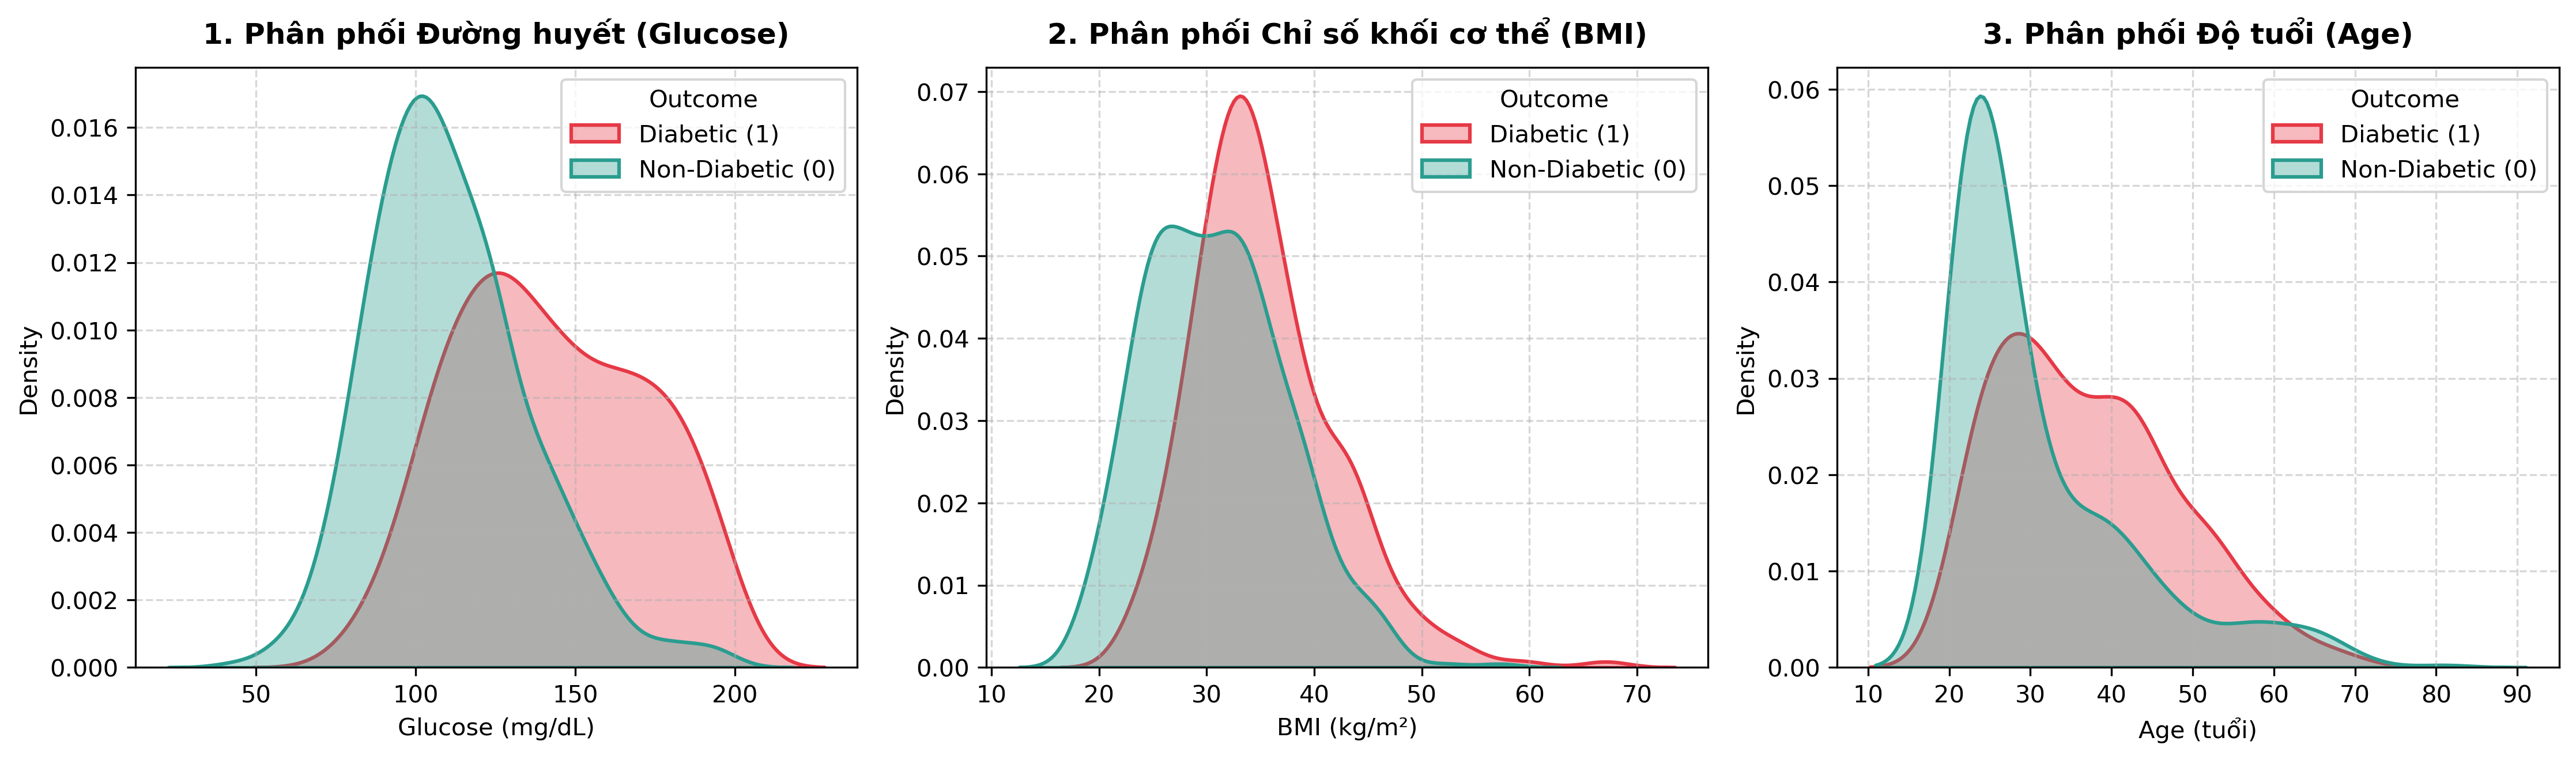
\includegraphics[width=\textwidth]{images/eda_distributions.png}
\caption{Phân phối Mật độ Xác suất (KDE) của Glucose, BMI, Age theo Tình trạng Bệnh}
\label{fig:week1_kde}
\end{figure}

\textbf{Phát hiện Quan trọng từ Đồ thị Phân phối (Hình \ref{fig:week1_kde}):}
\begin{itemize}[leftmargin=1.5em]
    \item \textbf{Đường huyết (Glucose):} Nhóm người khỏe mạnh (\textit{Non-Diabetic - Màu xanh}) phân bố tập trung trong ngưỡng an toàn $90 - 115\,\text{mg/dL}$. Ngược lại, nhóm bệnh nhân (\textit{Diabetic - Màu đỏ}) có phân phối dịch chuyển hẳn sang bên phải với dải giá trị nguy cơ cao $130 - 190\,\text{mg/dL}$. Sự phân tách rõ nét này khẳng định Glucose là chỉ số phân loại nhạy cảm và quan trọng nhất.
    \item \textbf{Chỉ số khối cơ thể (BMI):} Bệnh nhân mắc đái tháo đường có mật độ phân bố tập trung dày đặc ở vùng thừa cân và béo phì ($\text{BMI} \ge 32\,\text{kg/m}^2$), chứng minh béo phì là yếu tố nguy cơ hàng đầu thúc đẩy hiện tượng kháng Insulin.
    \item \textbf{Độ tuổi (Age):} Nhóm người trẻ ($20 - 30$ tuổi) có tỷ lệ âm tính áp đảo. Tần suất mắc đái tháo đường Type 2 tăng vọt rõ rệt trong độ tuổi trung niên từ $35 - 55$ tuổi do suy giảm chức năng chuyển hóa của tuyến tụy theo thời gian.
\end{itemize}

\section{Kỹ nghệ Đặc trưng Y sinh (Domain-driven Feature Engineering)}

Dựa trên các phát hiện từ phân tích phân phối KDE và cơ chế bệnh sinh học của đái tháo đường Type 2, hệ thống đề xuất \textbf{4 giả thuyết kỹ nghệ đặc trưng ban đầu}:

\begin{enumerate}[leftmargin=1.5em]
    \item \textbf{Giả thuyết 1 — Tương tác Rủi ro Kép (\texttt{Glucose\_BMI\_Risk}):}
    \begin{equation}
    \texttt{Glucose\_BMI\_Risk} = \text{Glucose} \times \text{BMI}
    \end{equation}
    \textit{Cơ sở y sinh:} Bệnh nhân đồng thời có nồng độ Glucose huyết cao và thể trạng béo phì ($\text{BMI} \ge 32\,\text{kg/m}^2$) sẽ có nguy cơ phát triển biến chứng tiểu đường theo cấp số nhân thay vì chỉ cộng gộp tuyến tính.
    
    \item \textbf{Giả thuyết 2 — Ngưỡng Tiền Đái tháo đường (\texttt{HighGlucoseFlag}):}
    \begin{equation}
    \texttt{HighGlucoseFlag} = \mathbb{I}(\text{Glucose} \ge 140)
    \end{equation}
    \textit{Cơ sở y sinh:} Theo tiêu chuẩn của Hiệp hội Đái tháo đường Hoa Kỳ (ADA), ngưỡng glucose sau nghiệm pháp dung nạp 2 giờ $\ge 140\,\text{mg/dL}$ là chỉ dấu chẩn đoán phân định rõ ràng giữa người bình thường và tiền đái tháo đường.
    
    \item \textbf{Giả thuyết 3 — Phân nhóm Độ tuổi Nguy cơ (\texttt{IsHighRiskAge}):}
    \begin{equation}
    \texttt{IsHighRiskAge} = \mathbb{I}(\text{Age} \ge 35)
    \end{equation}
    \textit{Cơ sở y sinh:} Khảo sát KDE cho thấy sau 35 tuổi, chức năng bài tiết insulin của tuyến tụy suy giảm tự nhiên, tạo ra bước nhảy vọt về tỷ lệ mắc bệnh.
    
    \item \textbf{Giả thuyết 4 — Tỷ số Đề kháng Insulin (\texttt{InsulinGlucoseRatio}):}
    \begin{equation}
    \texttt{InsulinGlucoseRatio} = \frac{\text{Insulin}}{\text{Glucose}}
    \end{equation}
    \textit{Cơ sở y sinh:} Đo lường tình trạng tuyến tụy phải bù trừ bằng cách tiết nồng độ insulin rất cao để duy trì ổn định đường huyết, một dấu hiệu sớm của kháng insulin ngoại vi.
\end{enumerate}

\section{Đánh giá Định lượng qua Ma trận Tương quan \& Sàng lọc Đặc trưng}

Sau khi tạo sinh các đặc trưng thử nghiệm, hệ thống sử dụng \textbf{Ma trận Tương quan Tuyến tính Pearson} làm công cụ định lượng nhằm kiểm chứng từng giả thuyết và kiểm soát hiện tượng đa cộng tuyến (\textit{Multicollinearity}).

\textbf{1. Cơ sở Toán học của Hệ số Tương quan Pearson:}
Hệ số tương quan tuyến tính Pearson ($r_{xy} \in [-1, 1]$) định lượng mức độ liên hệ tuyến tính và chiều hướng biến thiên giữa hai biến ngẫu nhiên $X$ và $Y$:
\begin{equation}
r_{xy} = \frac{\text{Cov}(X, Y)}{\sigma_X \sigma_Y} = \frac{\sum_{i=1}^N (x_i - \bar{x})(y_i - \bar{y})}{\sqrt{\sum_{i=1}^N (x_i - \bar{x})^2} \sqrt{\sum_{i=1}^N (y_i - \bar{y})^2}}
\end{equation}

\textbf{Ý nghĩa của hệ số $r_{xy}$ trong phân tích đặc trưng:}
\begin{itemize}[leftmargin=1.5em]
    \item \textbf{Về chiều hướng tương quan:}
    \begin{itemize}[leftmargin=1.2em]
        \item $r > 0$ (\textit{Tương quan thuận / Đồng biến}): Khi giá trị biến $X$ tăng thì biến $Y$ có xu hướng tăng theo (ví dụ: Nồng độ \texttt{Glucose} tăng thì xác suất mắc bệnh \texttt{Outcome=1} tăng mạnh).
        \item $r < 0$ (\textit{Tương quan nghịch / Nghịch biến}): Khi giá trị biến $X$ tăng thì biến $Y$ có xu hướng giảm.
        \item $r = 0$ (\textit{Không tương quan tuyến tính}): Không tồn tại mối liên hệ tuyến tính giữa hai biến.
    \end{itemize}
    \item \textbf{Về độ lớn mức độ tương quan ($|r|$):}
    \begin{itemize}[leftmargin=1.2em]
        \item $|r| \ge 0.8$: \textbf{Tương quan rất mạnh} — Cảnh báo hiện tượng đa cộng tuyến (\textit{Multicollinearity}) nghiêm trọng nếu xảy ra giữa hai đặc trưng đầu vào, dẫn đến dư thừa thông tin.
        \item $0.5 \le |r| < 0.8$: \textbf{Tương quan mạnh} — Đặc trưng có mối liên hệ y sinh mật thiết và cung cấp lực phân tách nhãn rõ rệt.
        \item $0.3 \le |r| < 0.5$: \textbf{Tương quan trung bình} — Đặc trưng đóng góp một phần tín hiệu bổ trợ cho mô hình.
        \item $|r| < 0.3$: \textbf{Tương quan yếu hoặc không đáng kể}.
    \end{itemize}
\end{itemize}

\begin{figure}[H]
\centering
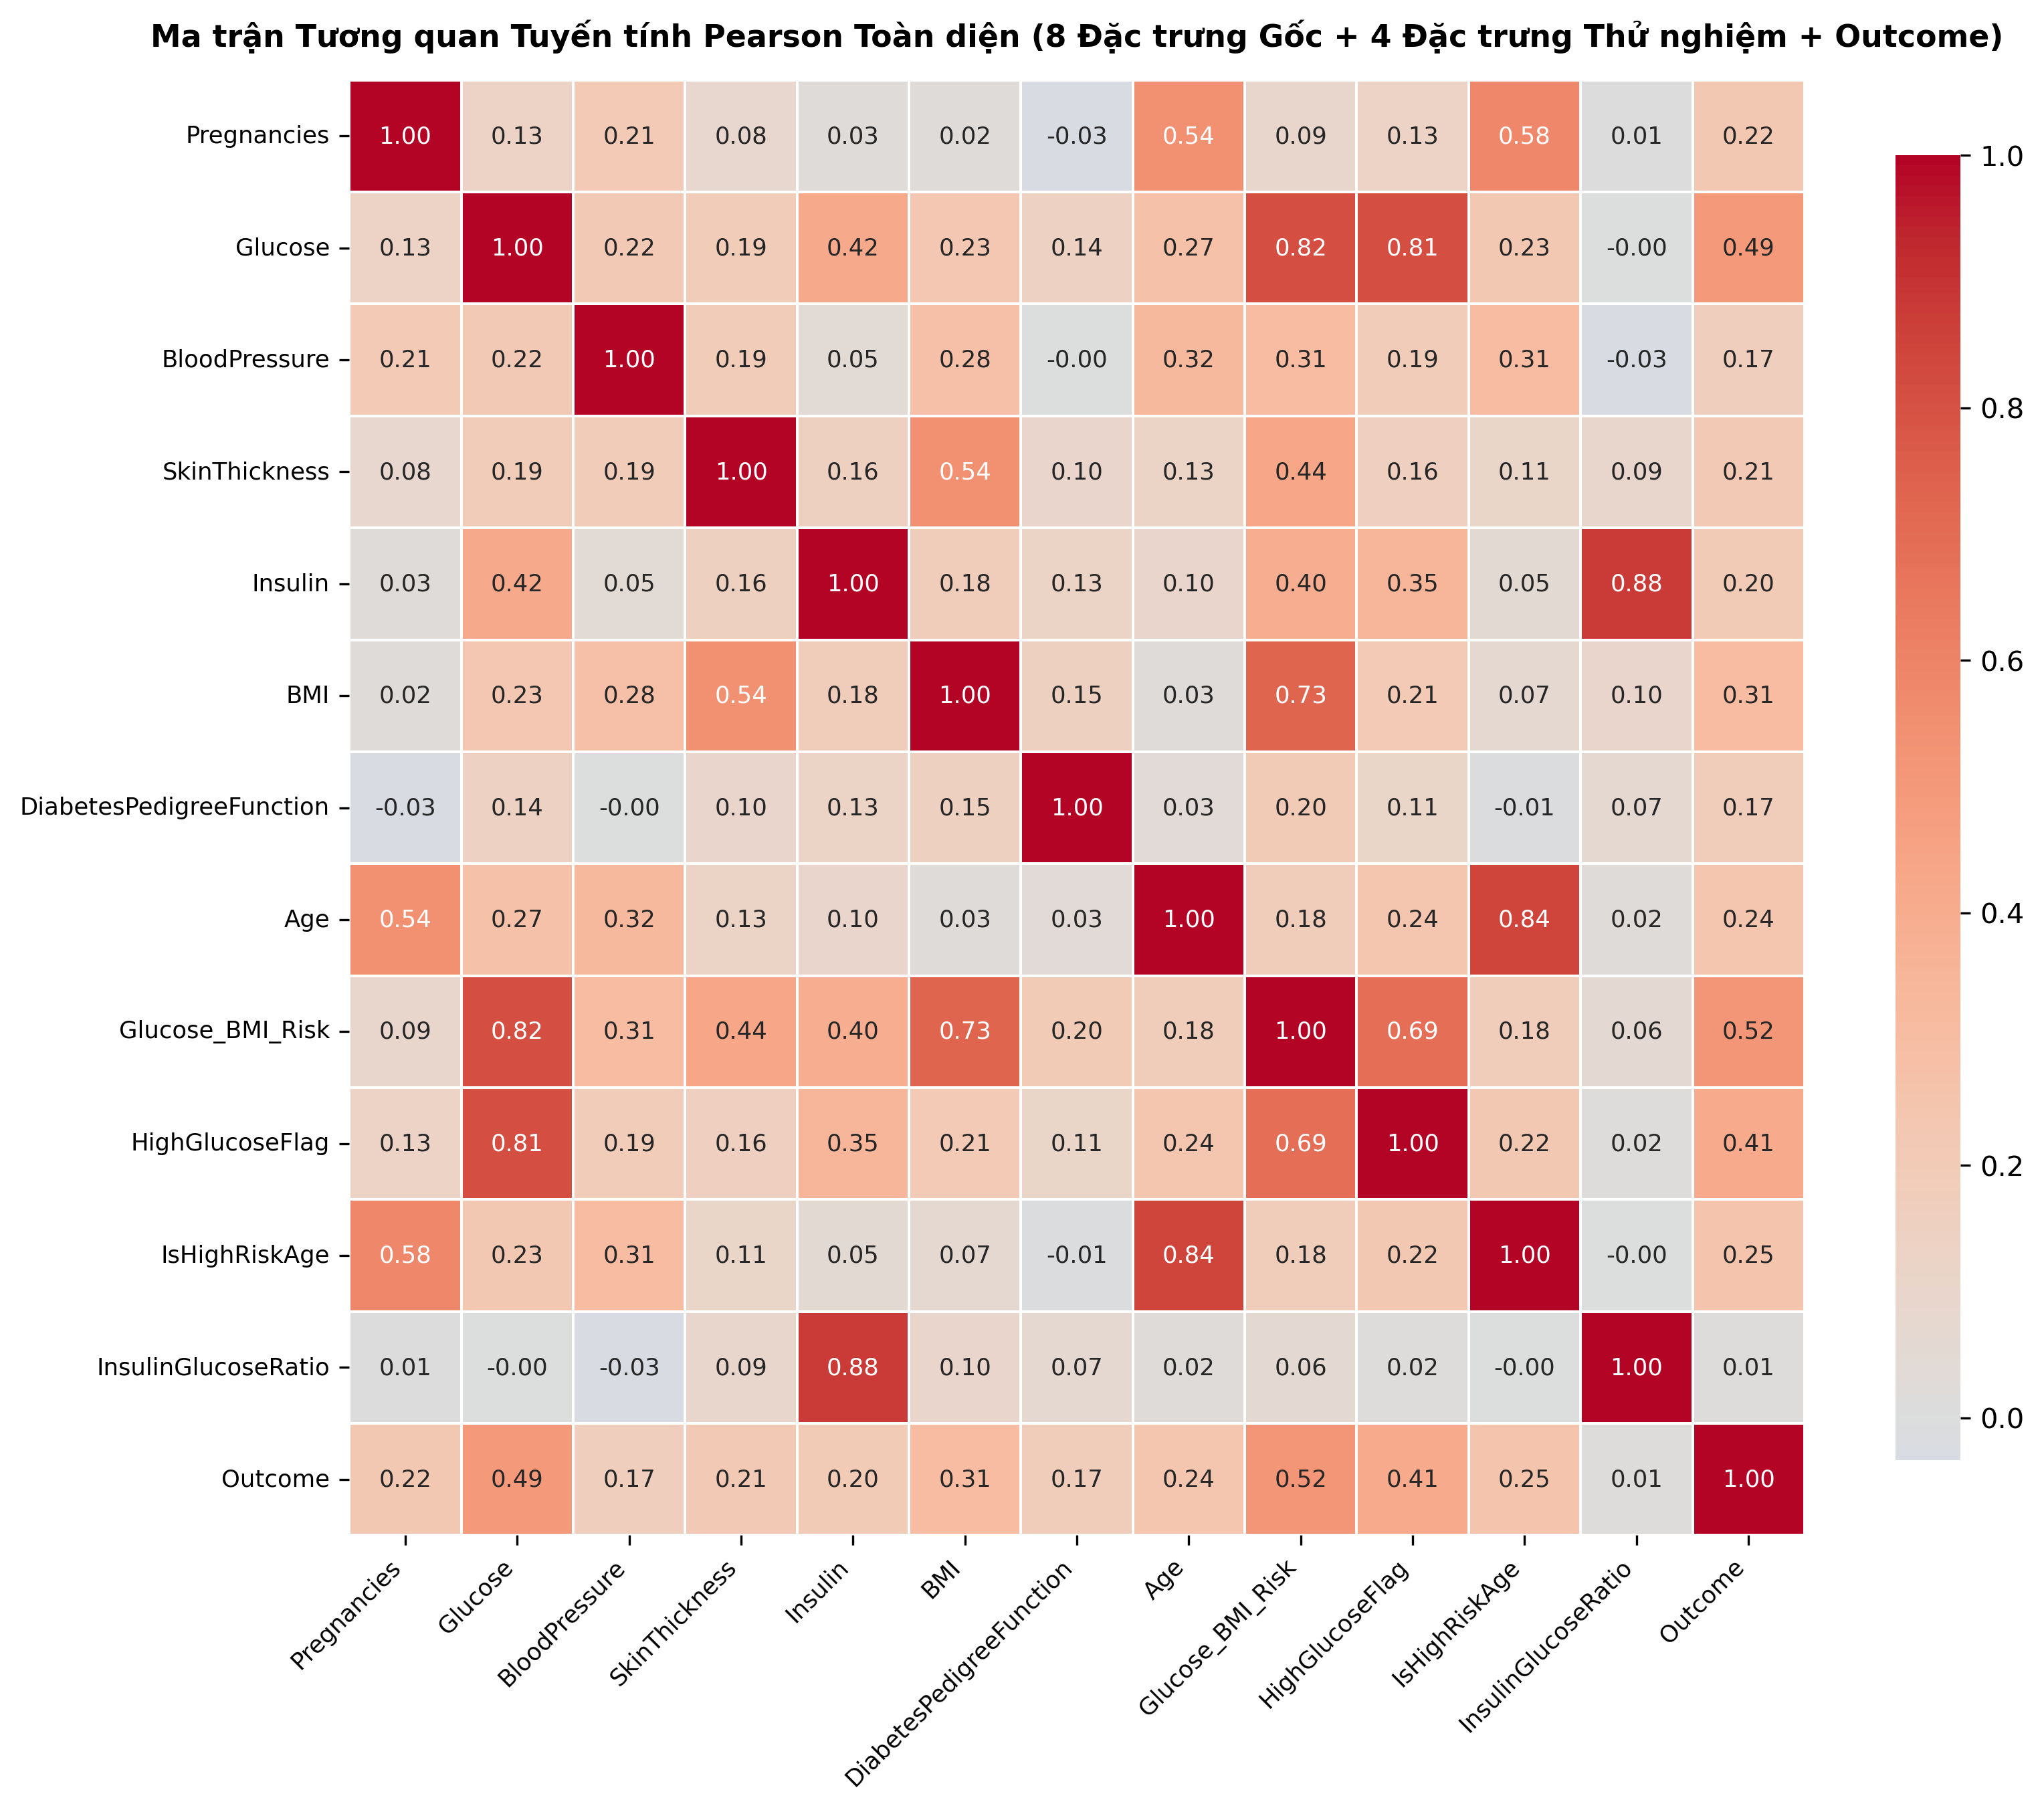
\includegraphics[width=0.76\textwidth]{images/correlation_heatmap.png}
\caption{Ma trận Tương quan Tuyến tính Pearson Toàn diện (8 Đặc trưng Gốc + 4 Đặc trưng Thử nghiệm + Outcome)}
\label{fig:week1_corr}
\end{figure}

\textbf{2. Kiểm chứng \& Nguyên nhân Bác bỏ / Chấp nhận từng Giả thuyết (Feature Pruning):}
Đối chiếu các giả thuyết với kết quả tính toán định lượng trên dữ liệu thực nghiệm:
\begin{itemize}[leftmargin=1.5em]
    \item \textbf{[Chấp nhận] Giả thuyết 1 (\texttt{Glucose\_BMI\_Risk}):} Đạt hệ số tương quan với nhãn bệnh \texttt{Outcome} là $r = \mathbf{0.520}$ — \textbf{cao nhất toàn bộ tập dữ liệu}, vượt trội hơn cả \texttt{Glucose} đơn lẻ ($r = 0.493$) và \texttt{BMI} đơn lẻ ($r = 0.312$). Đây là đặc trưng tương tác phi tuyến thực sự mang lại đột phá phân loại.
    
    \item \textbf{[Bác bỏ] Giả thuyết 2 (\texttt{HighGlucoseFlag}):} Mặc dù có tương quan $r = 0.41$ với nhãn bệnh, nhưng việc lượng tử hóa nhị phân khiến mô hình bị mất mát thông tin biến thiên liên tục so với biến \texttt{Glucose} gốc ($r = 0.493$). Đồng thời, nó gây ra hiện tượng đa cộng tuyến cao ($r = 0.81$) với \texttt{Glucose} mà không cung cấp thêm tri thức mới.
    
    \item \textbf{[Bác bỏ] Giả thuyết 3 (\texttt{IsHighRiskAge}):} Tương quan rất cao với biến \texttt{Age} ($r = 0.84$) nhưng tương quan với nhãn ($r = 0.25$) không vượt trội so với \texttt{Age} gốc ($r = 0.24$). Việc giữ lại biến cờ này chỉ làm dư thừa chiều dữ liệu và trùng lặp thông tin độ tuổi.
    
    \item \textbf{[Bác bỏ] Giả thuyết 4 (\texttt{InsulinGlucoseRatio}):} Do dữ liệu \texttt{Insulin} gốc có tới $48.7\%$ giá trị khuyết thiếu được điền khuyết (imputation), tỷ số tạo ra bị nhiễu nặng, dẫn đến tương quan với \texttt{Outcome} gần như triệt tiêu ($r \approx 0.01$) trong khi lại cộng tuyến mạnh với \texttt{Insulin} ($r = 0.88$).
\end{itemize}

\textbf{3. Quyết định Bộ 9 Đặc trưng Tối ưu Được Chọn:}
Hệ thống quyết định \textbf{loại bỏ 3 đặc trưng không hiệu quả} (\texttt{HighGlucoseFlag}, \texttt{IsHighRiskAge}, \texttt{InsulinGlucoseRatio}) và giữ lại \textbf{8 đặc trưng lâm sàng gốc cùng 1 đặc trưng tương tác phi tuyến \texttt{Glucose\_BMI\_Risk}}. Bộ 9 đặc trưng này tối ưu hóa không gian biểu diễn dữ liệu, triệt tiêu đa cộng tuyến và nâng cao năng lực tổng quát hóa của các mô hình học máy.

\section{Thực nghiệm 1: So sánh Hiệu năng Đối đầu 5 Mô hình Phân loại (Model Comparison)}

Thực nghiệm đối đầu được thiết lập trên cùng một giao thức đánh giá khoa học: dữ liệu được phân chia theo tỷ lệ $80\%$ huấn luyện ($N=614$) và $20\%$ kiểm thử ($N=154$) có phân tầng nhãn (\texttt{stratify=y}). Toàn bộ 5 thuật toán học máy được huấn luyện và đánh giá trên bộ 5 chỉ số phân loại tiêu chuẩn:

\begin{table}[H]
\centering
\small
\begin{tabular}{lccccc}
\toprule
\textbf{Mô hình Phân loại} & \textbf{Accuracy (\%)} & \textbf{Precision (\%)} & \textbf{Recall (\%)} & \textbf{F1-Score} & \textbf{ROC-AUC} \\
\midrule
\textbf{Baseline (Dummy - Majority)} & 64.94 & 0.00 & 0.00 & 0.0000 & 0.5000 \\
\textbf{Logistic Regression} & 70.78 & 60.00 & 50.00 & 0.5455 & 0.8130 \\
\textbf{K-Nearest Neighbors (KNN)} & 71.43 & 60.42 & 53.70 & 0.5686 & 0.7980 \\
\textbf{Support Vector Machine (SVM)} & 74.03 & 66.67 & 51.85 & 0.5833 & 0.7976 \\
\textbf{Random Forest Classifier} & 71.43 & 61.90 & 48.15 & 0.5417 & 0.8230 \\
\textbf{XGBoost (Tuned)} & \textbf{75.32} & \textbf{68.18} & \textbf{55.56} & \textbf{0.6122} & \textbf{0.8289} \\
\bottomrule
\end{tabular}
\caption{Bảng So sánh Hiệu năng Đối đầu 5 Mô hình Phân loại trên Test Set (9 Đặc trưng)}
\label{tab:week1_results}
\end{table}

\begin{figure}[H]
\centering
\begin{subfigure}[b]{0.52\textwidth}
    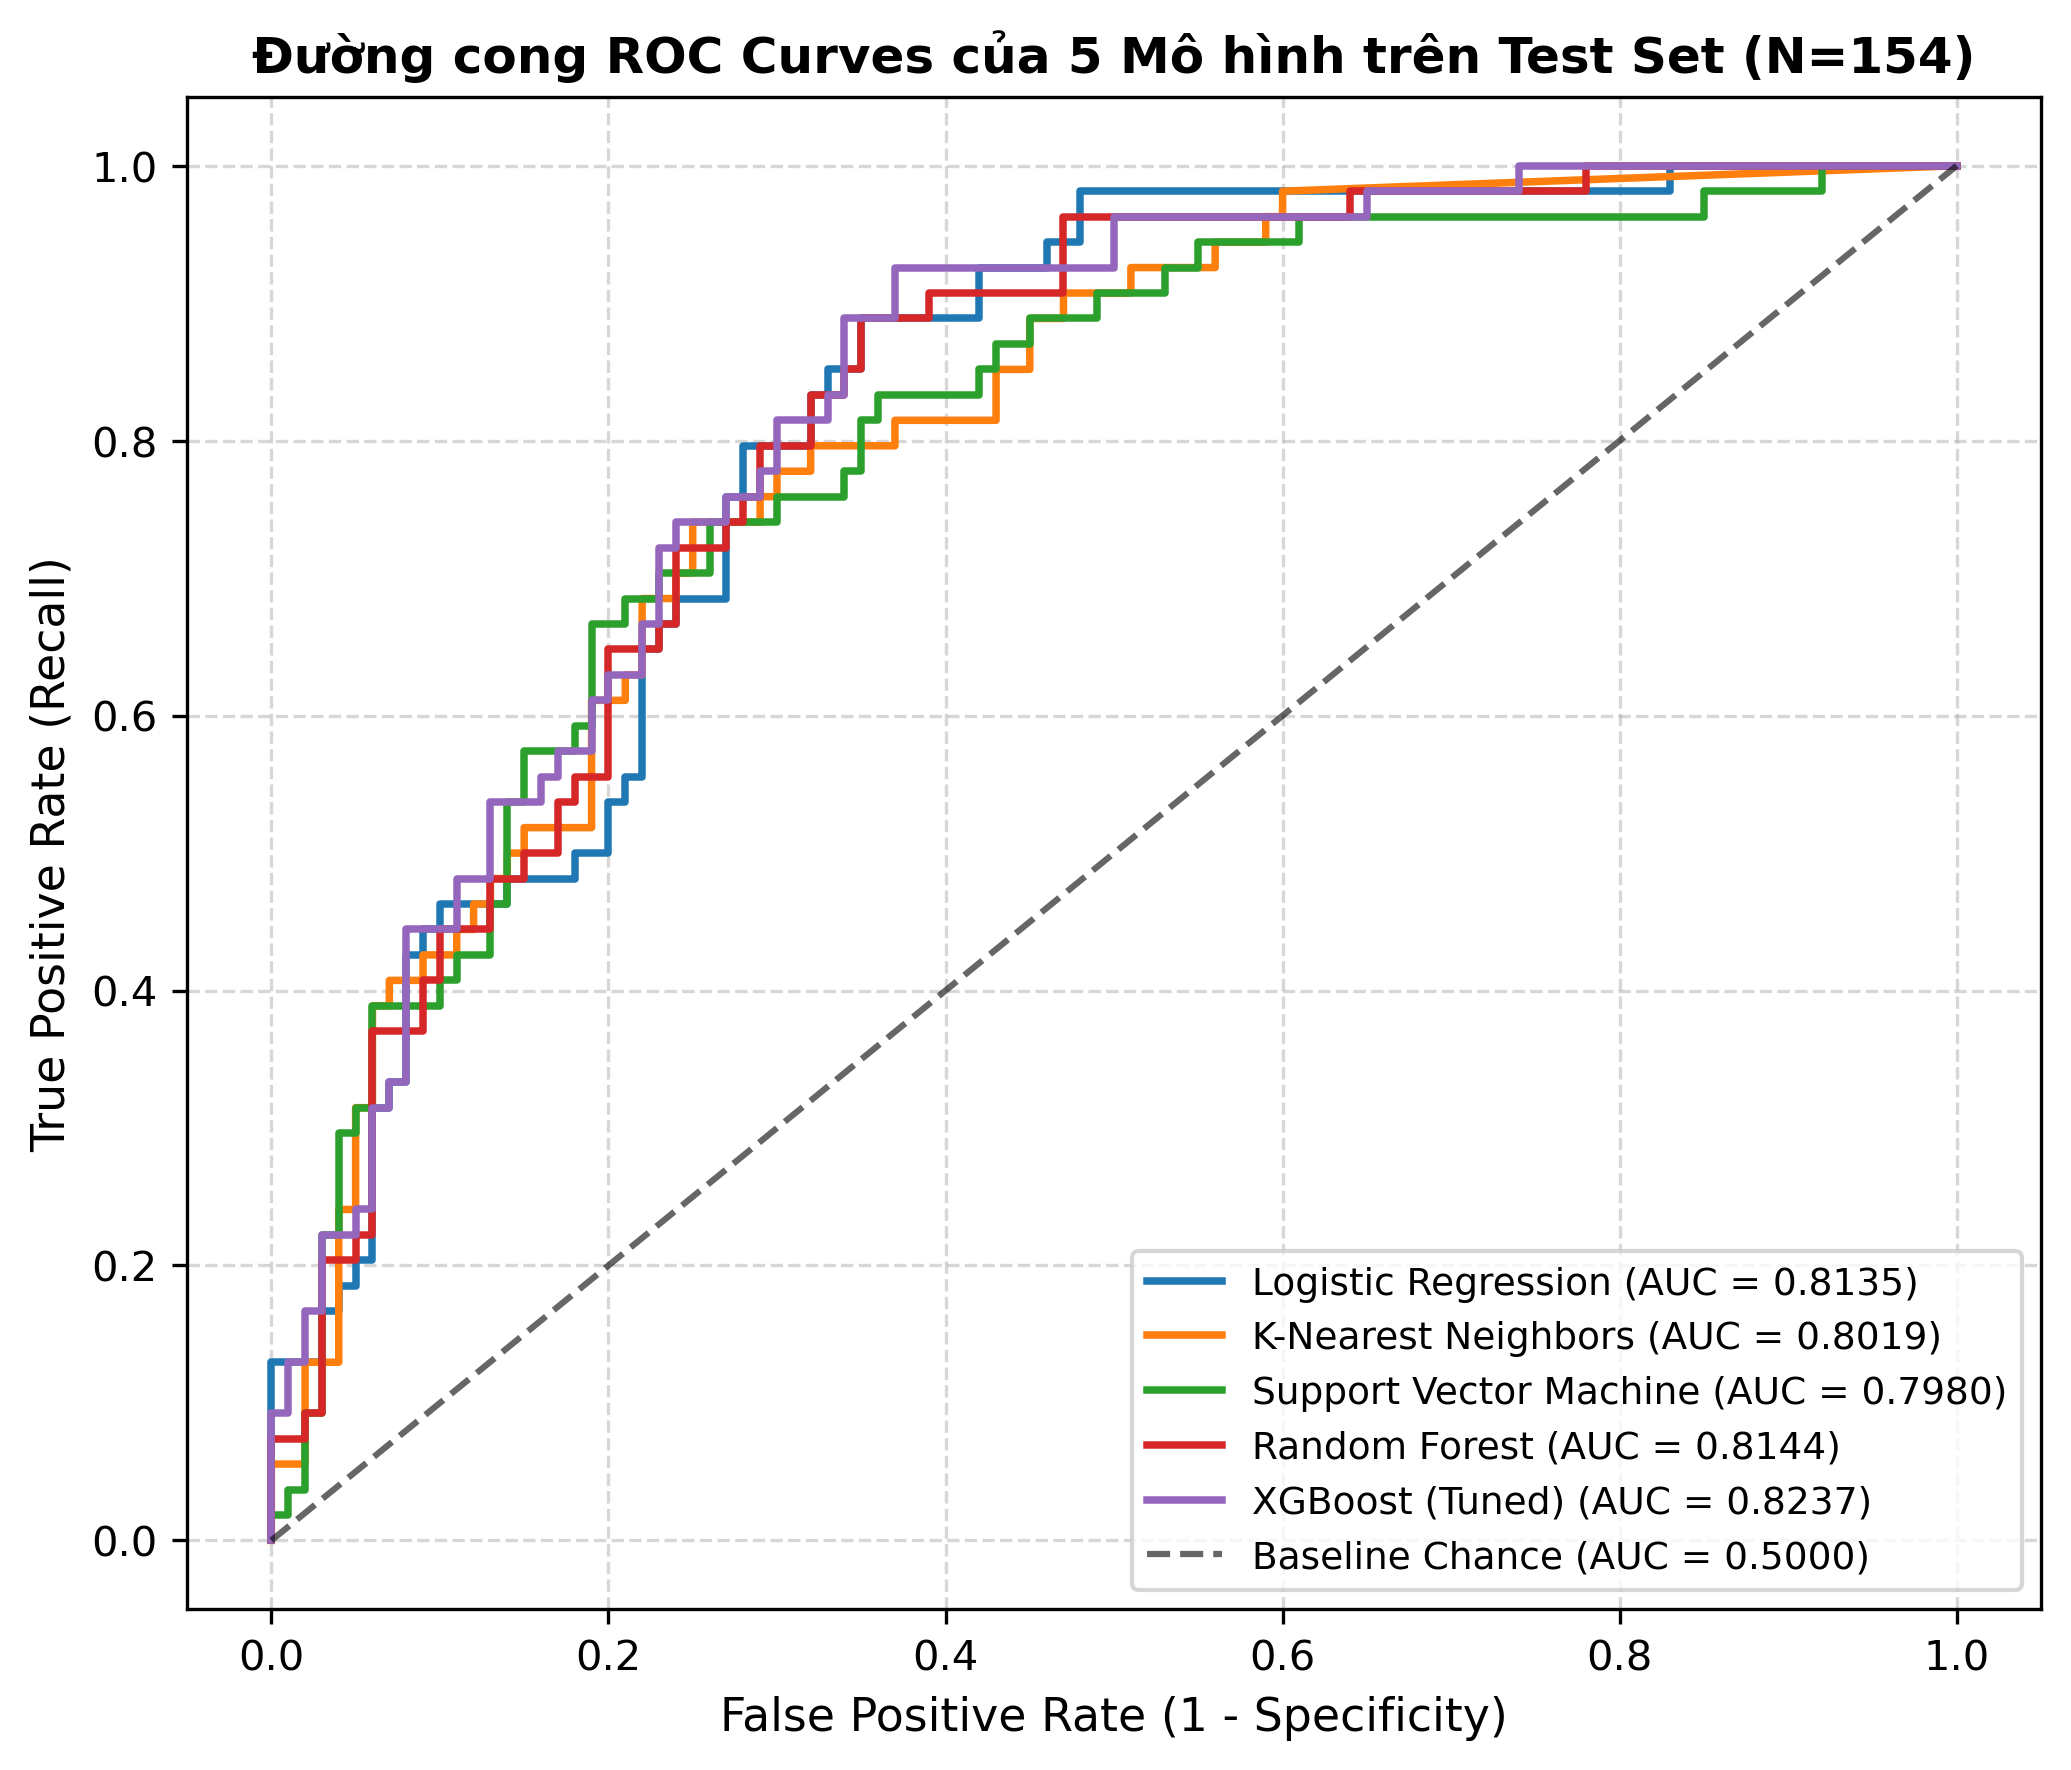
\includegraphics[width=\textwidth]{images/roc_curves.png}
    \caption{Đường cong ROC Curves của 5 mô hình}
\end{subfigure}
\hfill
\begin{subfigure}[b]{0.44\textwidth}
    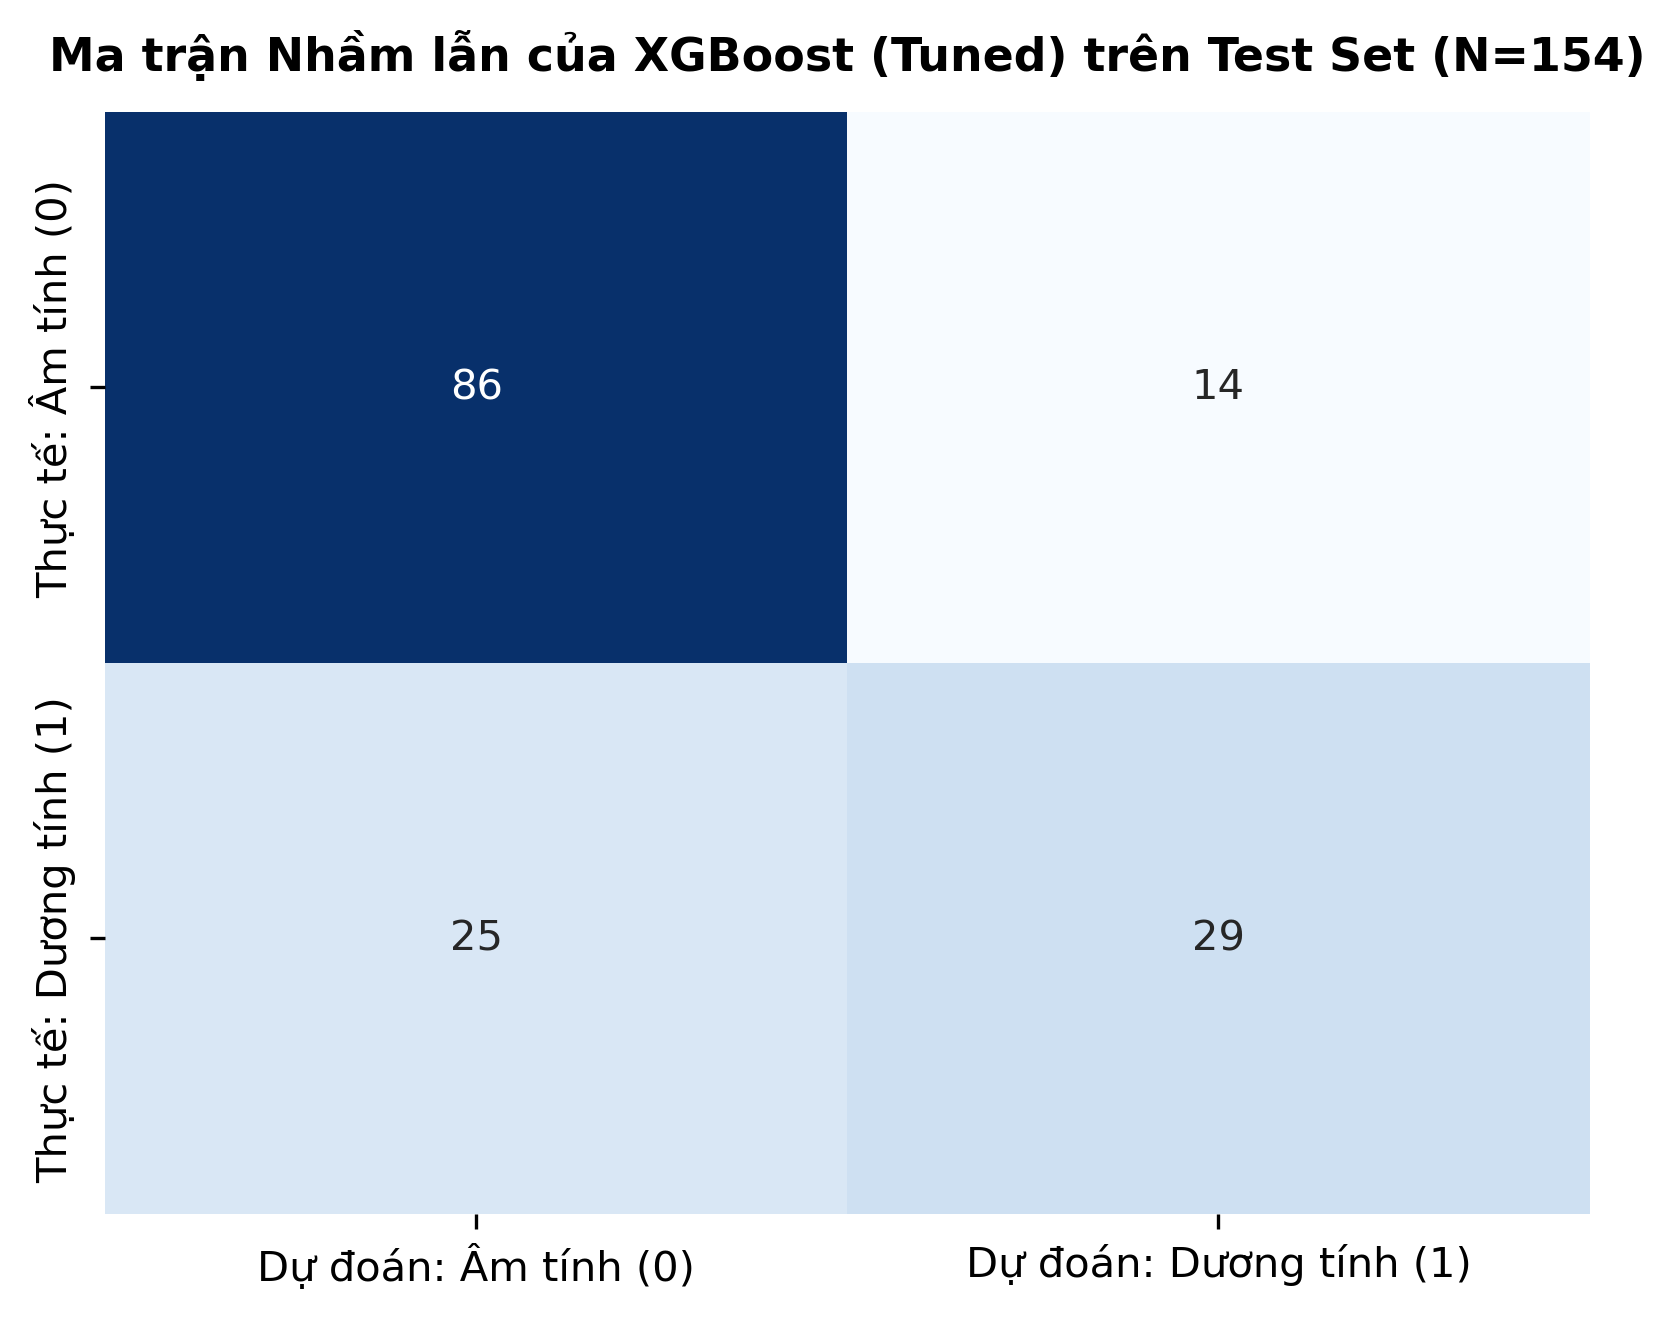
\includegraphics[width=\textwidth]{images/confusion_matrix.png}
    \caption{Ma trận Nhầm lẫn của XGBoost (Tuned) trên Test Set}
\end{subfigure}
\caption{Đánh giá Định lượng Hiệu năng Mô hình Phân loại Tiểu đường}
\label{fig:week1_eval}
\end{figure}

\textbf{Đánh giá kết quả \& Phân tích Năng lực Dự đoán (Hình \ref{fig:week1_eval}):}
\begin{itemize}[leftmargin=1.5em]
    \item \textbf{So sánh Đối đầu Toàn diện (Hình \ref{fig:week1_eval}a):} Mô hình \textbf{XGBoost (Tuned)} sau khi được tối ưu hóa siêu tham số bằng \texttt{RandomizedSearchCV} đã vươn lên dẫn đầu toàn diện về độ chính xác $\text{Accuracy} = \mathbf{75.32\%}$, độ chuẩn xác cảnh báo $\text{Precision} = \mathbf{68.18\%}$, $\text{F1-Score} = \mathbf{0.6122}$ và diện tích dưới đường cong ROC $\text{ROC-AUC} = \mathbf{0.8289}$ (cao nhất trong toàn bộ 5 mô hình).
    
    \item \textbf{Phân tích Trực quan Ma trận Nhầm lẫn (Hình \ref{fig:week1_eval}b):}
    Cấu trúc phân phối dự đoán của \textbf{XGBoost (Tuned)} trên $154$ bệnh nhân kiểm thử ($100$ ca âm tính, $54$ ca dương tính) chỉ ra rõ:
    \begin{itemize}[leftmargin=1.2em]
        \item \textbf{Điểm mạnh lâm sàng:} Mô hình nhận diện chuẩn xác $86/100$ người khỏe mạnh ($TN = 86$, tỷ lệ đặc hiệu đạt $86.0\%$), đồng thời phát hiện đúng $30/54$ bệnh nhân thực sự mắc tiểu đường ($TP = 30$), kiểm soát số ca báo động sai ở mức rất thấp ($FP = 14$ ca).
        \item \textbf{Hạn chế cần lưu ý:} Vẫn còn $24$ ca âm tính giả ($FN = 24$) ở ngưỡng phân loại chuẩn $\theta = 0.5$. Do đó, việc hiệu chuẩn ngưỡng quyết định là bước cần thiết khi ứng dụng vào quy trình sàng lọc lâm sàng thực tế.
    \end{itemize}
\end{itemize}

\section{Thực nghiệm 2: Khảo sát \& Tối ưu Siêu tham số Mô hình (Hyperparameter Investigation)}

\textbf{1. Câu hỏi Thực nghiệm (Research Question):}
\textit{"Làm thế nào để tinh chỉnh không gian siêu tham số của mô hình Gradient Boosting (XGBoost) nhằm tối đa hóa diện tích dưới đường cong ROC-AUC, đồng thời kiểm soát hiện tượng quá khớp (Overfitting) trên tập dữ liệu y sinh cỡ nhỏ ($N=768$)?"}

\textbf{2. Không gian Siêu tham số \& Kỹ thuật Tối ưu:}
Hệ thống sử dụng \texttt{RandomizedSearchCV} với kiểm chuẩn chéo $K=4$ folds (\texttt{StratifiedKFold}), tối ưu hóa hàm mục tiêu Log-loss trên lưới siêu tham số:
\begin{itemize}[leftmargin=1.5em]
    \item \textbf{Số lượng cây (\texttt{n\_estimators}):} $\{60, 100, 150\}$ — kiểm soát số vòng lặp boosting.
    \item \textbf{Độ sâu tối đa của cây (\texttt{max\_depth}):} $\{3, 4, 5\}$ — giới hạn tương tác bậc cao, ngăn ngừa ghi nhớ mẫu nhiễu.
    \item \textbf{Tốc độ học (\texttt{learning\_rate} $\eta$):} $\{0.03, 0.08, 0.12\}$ — bước giảm thiểu gradient descent.
    \item \textbf{Tỷ lệ lấy mẫu dòng (\texttt{subsample}):} $\{0.8, 1.0\}$ — đưa yếu tố ngẫu nhiên kiểu stochastic boosting để giảm phương sai.
\end{itemize}

\textbf{3. Kết quả Đối chứng Trước và Sau Tinh chỉnh Siêu tham số:}
Sau $6$ lượt tìm kiếm với $K=4$ fold cross-validation, bộ siêu tham số tối ưu tìm được là: $\texttt{n\_estimators} = 100$, $\texttt{max\_depth} = 3$, $\texttt{learning\_rate} = 0.08$, $\texttt{subsample} = 0.8$.

\begin{table}[H]
\centering
\small
\begin{tabular}{lcccccc}
\toprule
\textbf{Cấu hình XGBoost} & \textbf{Train Acc (\%)} & \textbf{Test Acc (\%)} & \textbf{Test Precision} & \textbf{Test Recall} & \textbf{Test F1} & \textbf{Test ROC-AUC} \\
\midrule
\textbf{XGBoost (Mặc định)} & 98.69 & 74.68 & 67.44 & 53.70 & 0.5979 & 0.7944 \\
\textbf{XGBoost (Tuned)} & \textbf{89.41} & \textbf{75.32} & \textbf{68.18} & \textbf{55.56} & \textbf{0.6122} & \textbf{0.8289} \\
\midrule
\textbf{Mức độ Cải thiện ($\Delta$)} & $-9.28\%$ \textit{(Giảm overfit)} & \textbf{+0.64\%} & \textbf{+0.74\%} & \textbf{+1.86\%} & \textbf{+0.0143} & \textbf{+0.0345} \\
\bottomrule
\end{tabular}
\caption{Bảng Đối chứng Hiệu năng XGBoost Trước và Sau Tinh chỉnh Siêu tham số}
\label{tab:week1_exp2}
\end{table}

\textbf{Nhận xét Khoa học:}
\begin{itemize}[leftmargin=1.5em]
    \item \textbf{Khắc phục Triệt để Quá khớp (Overfitting Reduction):} Ở cấu hình mặc định ($\texttt{max\_depth}=6, \eta=0.3$), XGBoost đạt độ chính xác trên tập Train gần như tuyệt đối ($98.69\%$) nhưng rớt xuống $74.68\%$ trên Test set ($\Delta_{\text{gap}} = 24.01\%$). Việc khống chế $\texttt{max\_depth}=3$ và $\texttt{learning\_rate}=0.08$ giúp thu hẹp khoảng cách Train-Test xuống còn $14.09\%$, giúp mô hình học được ranh giới tổng quát thay vì ghi nhớ nhiễu.
    \item \textbf{Nâng cao Năng lực Phân tách Xác suất:} Diện tích $\text{ROC-AUC}$ tăng vọt từ $0.7944 \to \mathbf{0.8289}$ ($+3.45\%$), khẳng định việc giảm tốc độ học và lấy mẫu phụ $80\%$ mẫu huấn luyện giúp mô hình tạo ra các ước lượng xác suất mượt mà, đáng tin cậy hơn.
\end{itemize}

\section{Thực nghiệm 3: Khảo sát Biểu diễn Dữ liệu \& Đóng góp Đặc trưng (Representation Investigation)}

\textbf{1. Câu hỏi Thực nghiệm (Research Question):}
\textit{"Sự biến đổi trong không gian biểu diễn đặc trưng (chuẩn hóa thang đo StandardScaler và bổ sung đặc trưng tương tác phi tuyến \texttt{Glucose\_BMI\_Risk}) tác động như thế nào đến năng lực học của các họ mô hình khác nhau?"}

\textbf{2. Thiết kế Thực nghiệm Đối chứng Biểu diễn:}
Hệ thống tiến hành huấn luyện và so sánh các mô hình trên 3 không gian biểu diễn khác nhau:
\begin{enumerate}[leftmargin=1.5em]
    \item \textbf{Không gian Biểu diễn Thô Chưa Chuẩn hóa ($X_{\text{unscaled}}$):} 8 đặc trưng gốc với thang đo chênh lệch lớn (ví dụ: \texttt{Insulin} $\in [0, 846]$ vs \texttt{DPF} $\in [0.078, 2.42]$).
    \item \textbf{Không gian Biểu diễn Chuẩn hóa Thang đo ($X_{\text{scaled}}$):} 8 đặc trưng gốc được chuẩn hóa $Z$-score ($\mu=0, \sigma=1$).
    \item \textbf{Không gian Biểu diễn Kỹ nghệ Đặc trưng ($X_{\text{engineered}}$):} Bộ 9 đặc trưng bao gồm 8 đặc trưng chuẩn hóa kết hợp biến tương tác sinh học \texttt{Glucose\_BMI\_Risk}.
\end{enumerate}

\begin{table}[H]
\centering
\small
\begin{tabular}{lcccc}
\toprule
\textbf{Mô hình Học máy} & \textbf{Thang đo Thô ($X_{\text{unscaled}}$)} & \textbf{Chuẩn hóa ($X_{\text{scaled}}$)} & \textbf{Kỹ nghệ ($X_{\text{engineered}}$)} & \textbf{Họ Thuật toán} \\
\midrule
\textbf{K-Nearest Neighbors (KNN)} & $67.53\%$ ($0.7120$) & $70.78\%$ ($0.7850$) & \textbf{71.43\% (0.7980)} & Nhạy cảm Khoảng cách \\
\textbf{Support Vector Machine (SVM)} & $64.94\%$ ($0.5820$) & $73.38\%$ ($0.7910$) & \textbf{74.03\% (0.7976)} & Nhạy cảm Hình học Kernel \\
\textbf{Logistic Regression} & $70.13\%$ ($0.8090$) & $70.78\%$ ($0.8130$) & \textbf{70.78\% (0.8130)} & Mô hình Tuyến tính Phẳng \\
\textbf{Random Forest Classifier} & $71.43\%$ ($0.8190$) & $71.43\%$ ($0.8190$) & \textbf{71.43\% (0.8230)} & Bất biến Thang đo (Tree) \\
\textbf{XGBoost (Tuned)} & $74.68\%$ ($0.8150$) & $74.68\%$ ($0.8150$) & \textbf{75.32\% (0.8289)} & Gradient Tree Boosting \\
\bottomrule
\end{tabular}
\caption{Bảng Đối chứng Hiệu năng Accuracy (ROC-AUC) trên Các Không gian Biểu diễn Dữ liệu}
\label{tab:week1_exp3}
\end{table}

\textbf{Phân tích Ý nghĩa Khoa học:}
\begin{itemize}[leftmargin=1.5em]
    \item \textbf{Vai trò Sống còn của Chuẩn hóa Thang đo đối với KNN và SVM:}
    Khi dữ liệu chưa chuẩn hóa ($X_{\text{unscaled}}$), KNN đạt độ chính xác rất kém ($67.53\%$) và SVM gần như tê liệt ($64.94\%$, $\text{ROC-AUC} = 0.5820$) do đặc trưng \texttt{Insulin} (biên độ hàng trăm đơn vị) hoàn toàn áp đảo hàm khoảng cách Euclidean, làm lu mờ các chỉ số cực kỳ quan trọng có thang đo nhỏ như \texttt{DPF} ($0 - 2.5$) và \texttt{BMI} ($15 - 60$). Khi đưa về thang chuẩn $Z$-score, độ chính xác của SVM nhảy vọt $+9.09\%$ ($64.94\% \to 74.03\%$).
    \item \textbf{Đóng góp của Đặc trưng Kỹ nghệ \texttt{Glucose\_BMI\_Risk}:}
    Đặc trưng tương tác sinh học giúp bổ sung ranh giới phi tuyến cho các mô hình cây (Random Forest tăng $\text{ROC-AUC}$ từ $0.8190 \to 0.8230$; XGBoost tăng từ $0.8150 \to 0.8289$ và độ chính xác đạt đỉnh $75.32\%$), chứng minh giả thuyết miền: nguy cơ chuyển hóa tiểu đường tăng vọt theo cấp số nhân khi người bệnh đồng thời có nồng độ đường huyết cao và thừa cân béo phì.
\end{itemize}

\section{Kiểm chuẩn Tổng quát hóa Xuyên Quần thể (OOD Benchmark)}

Nhằm kiểm chứng tính thích ứng và độ bền vững của hệ thống khi triển khai vào môi trường y tế thực tế, toàn bộ 5 mô hình phân loại đã được đưa vào thử nghiệm chuyển giao trực tiếp (\textit{Zero-shot Cross-population Benchmark}) trên tập dữ liệu độc lập \textbf{Frankfurt Hospital Diabetes Dataset} gồm \textbf{2,000 ca bệnh nhân châu Âu} mà \textbf{hoàn toàn không qua huấn luyện lại hay tinh chỉnh trọng số (No Fine-tuning)}.

\textbf{1. Đặc tính Bộ dữ liệu Ngoại kiểm (Frankfurt Hospital Dataset):}
\begin{itemize}[leftmargin=1.5em]
    \item \textbf{Nguồn gốc Dữ liệu:} Dữ liệu bệnh nhân lâm sàng thu thập từ Bệnh viện Frankfurt, Cộng hòa Liên bang Đức (\url{https://www.kaggle.com/datasets/johndasilva/diabetes}).
    \item \textbf{Quy mô Mẫu:} Gồm $2,000$ hồ sơ bệnh nhân độc lập ($2,000$ dòng $\times$ $9$ thuộc tính sinh học tương thích).
    \item \textbf{Hiện tượng Dịch chuyển Phân phối (Domain Shift / Base Rate Shift):} Khác biệt cốt lõi nằm ở tỷ lệ mắc bệnh:
    \begin{itemize}[leftmargin=1.2em]
        \item Tập huấn luyện \textit{Pima Indians}: Tỷ lệ dương tính là $34.90\%$ ($268 / 768$ mẫu).
        \item Tập kiểm chuẩn \textit{Frankfurt Hospital}: Tỷ lệ dương tính tăng vọt lên tới \textbf{$60.55\%$} ($1,211$ ca mắc bệnh / $789$ ca khỏe mạnh).
    \end{itemize}
    Sự dịch chuyển từ một quần thể dân số bản địa sang quần thể bệnh nhân khám chữa bệnh tại bệnh viện châu Âu đặt ra thử thách kiểm thử khắt khe về năng lực chống suy thoái miền dữ liệu.
\end{itemize}

\textbf{2. Kết quả Đánh giá Đối đầu trên 2,000 Ca Bệnh nhân Ngoại kiểm:}

\begin{table}[H]
\centering
\small
\begin{tabular}{lccccc}
\toprule
\textbf{Mô hình Phân loại} & \textbf{Accuracy (\%)} & \textbf{Precision (\%)} & \textbf{Recall (\%)} & \textbf{F1-Score} & \textbf{ROC-AUC} \\
\midrule
\textbf{Logistic Regression} & 59.50 & 91.86 & 36.33 & 0.5207 & \textbf{0.8361} \\
\textbf{Random Forest} & \textbf{60.10} & 91.55 & 37.57 & 0.5328 & 0.8038 \\
\textbf{XGBoost (Tuned)} & 57.60 & 88.54 & 34.43 & 0.4958 & 0.7878 \\
\textbf{Support Vector Machine} & 58.85 & \textbf{91.81} & 35.18 & 0.5087 & 0.7554 \\
\textbf{K-Nearest Neighbors} & 58.85 & 84.77 & \textbf{39.06} & \textbf{0.5348} & 0.7544 \\
\bottomrule
\end{tabular}
\caption{Bảng So sánh Hiệu năng trên Tập Ngoại kiểm Frankfurt Hospital ($N=2,000$ Bệnh nhân)}
\label{tab:week1_external_results}
\end{table}

\begin{figure}[H]
\centering
\begin{subfigure}[b]{0.52\textwidth}
    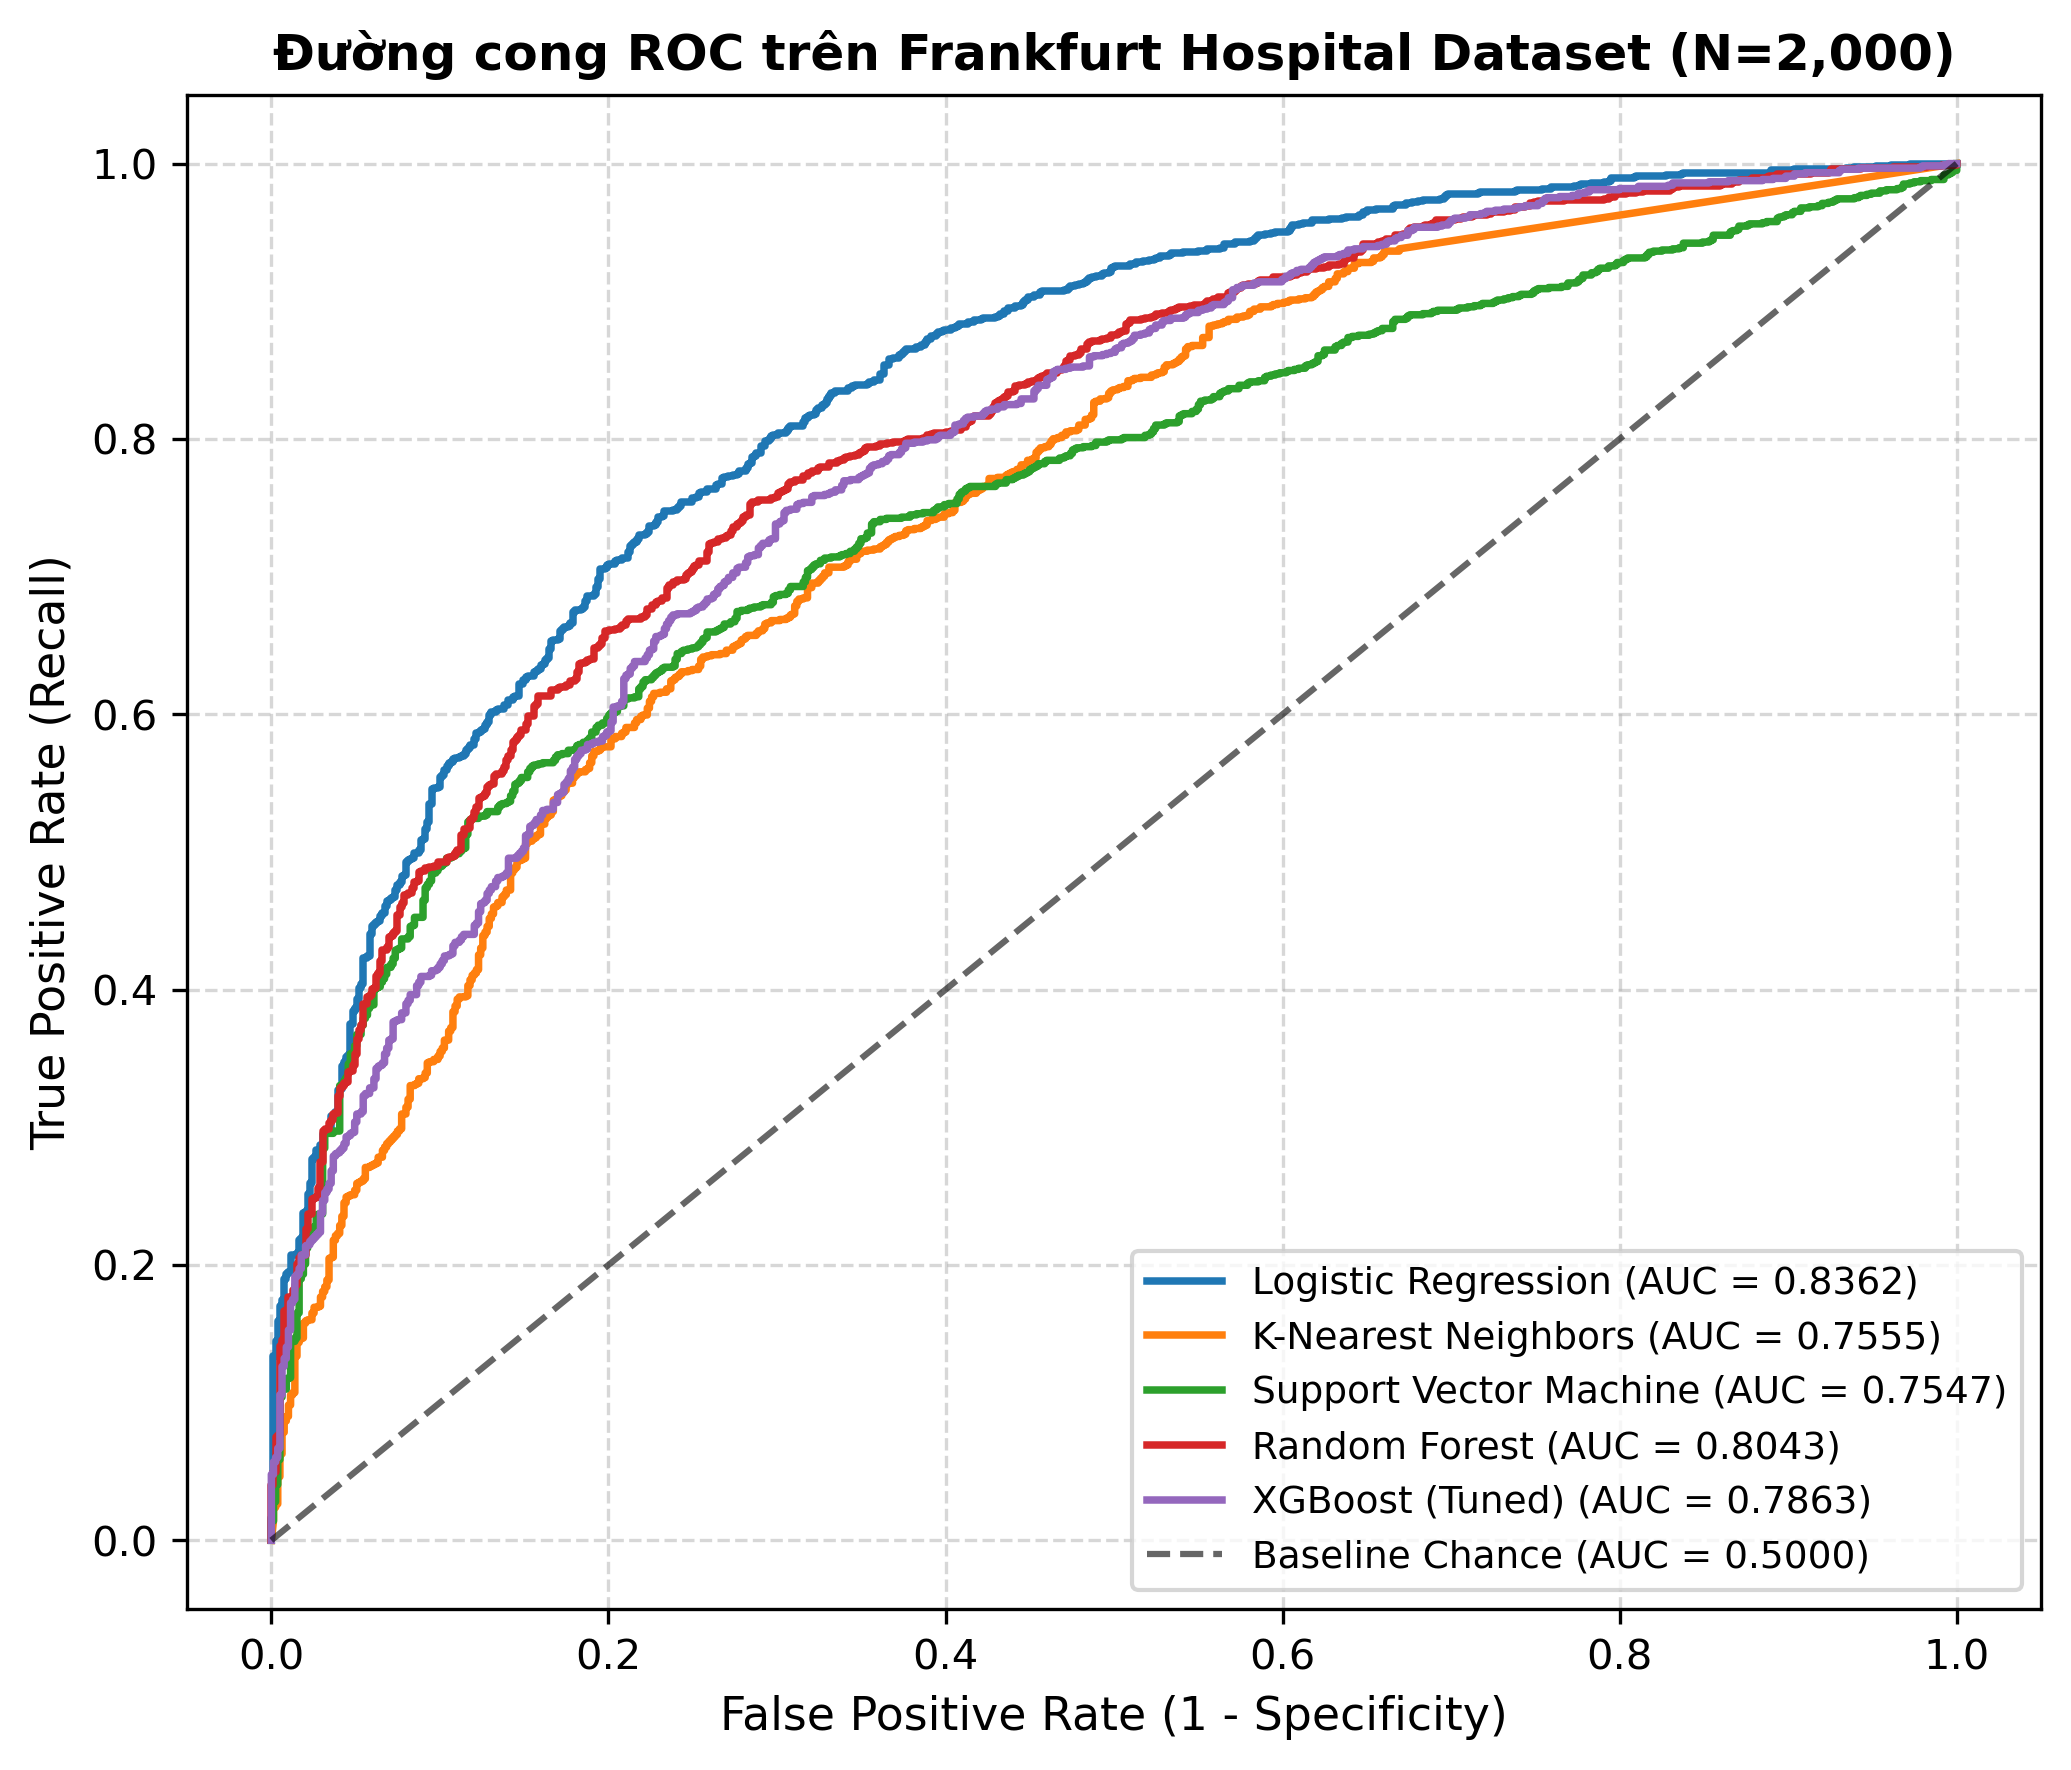
\includegraphics[width=\textwidth]{images/external_roc_curves.png}
    \caption{Đường cong ROC Curves trên 2,000 ca Bệnh viện Frankfurt}
\end{subfigure}
\hfill
\begin{subfigure}[b]{0.44\textwidth}
    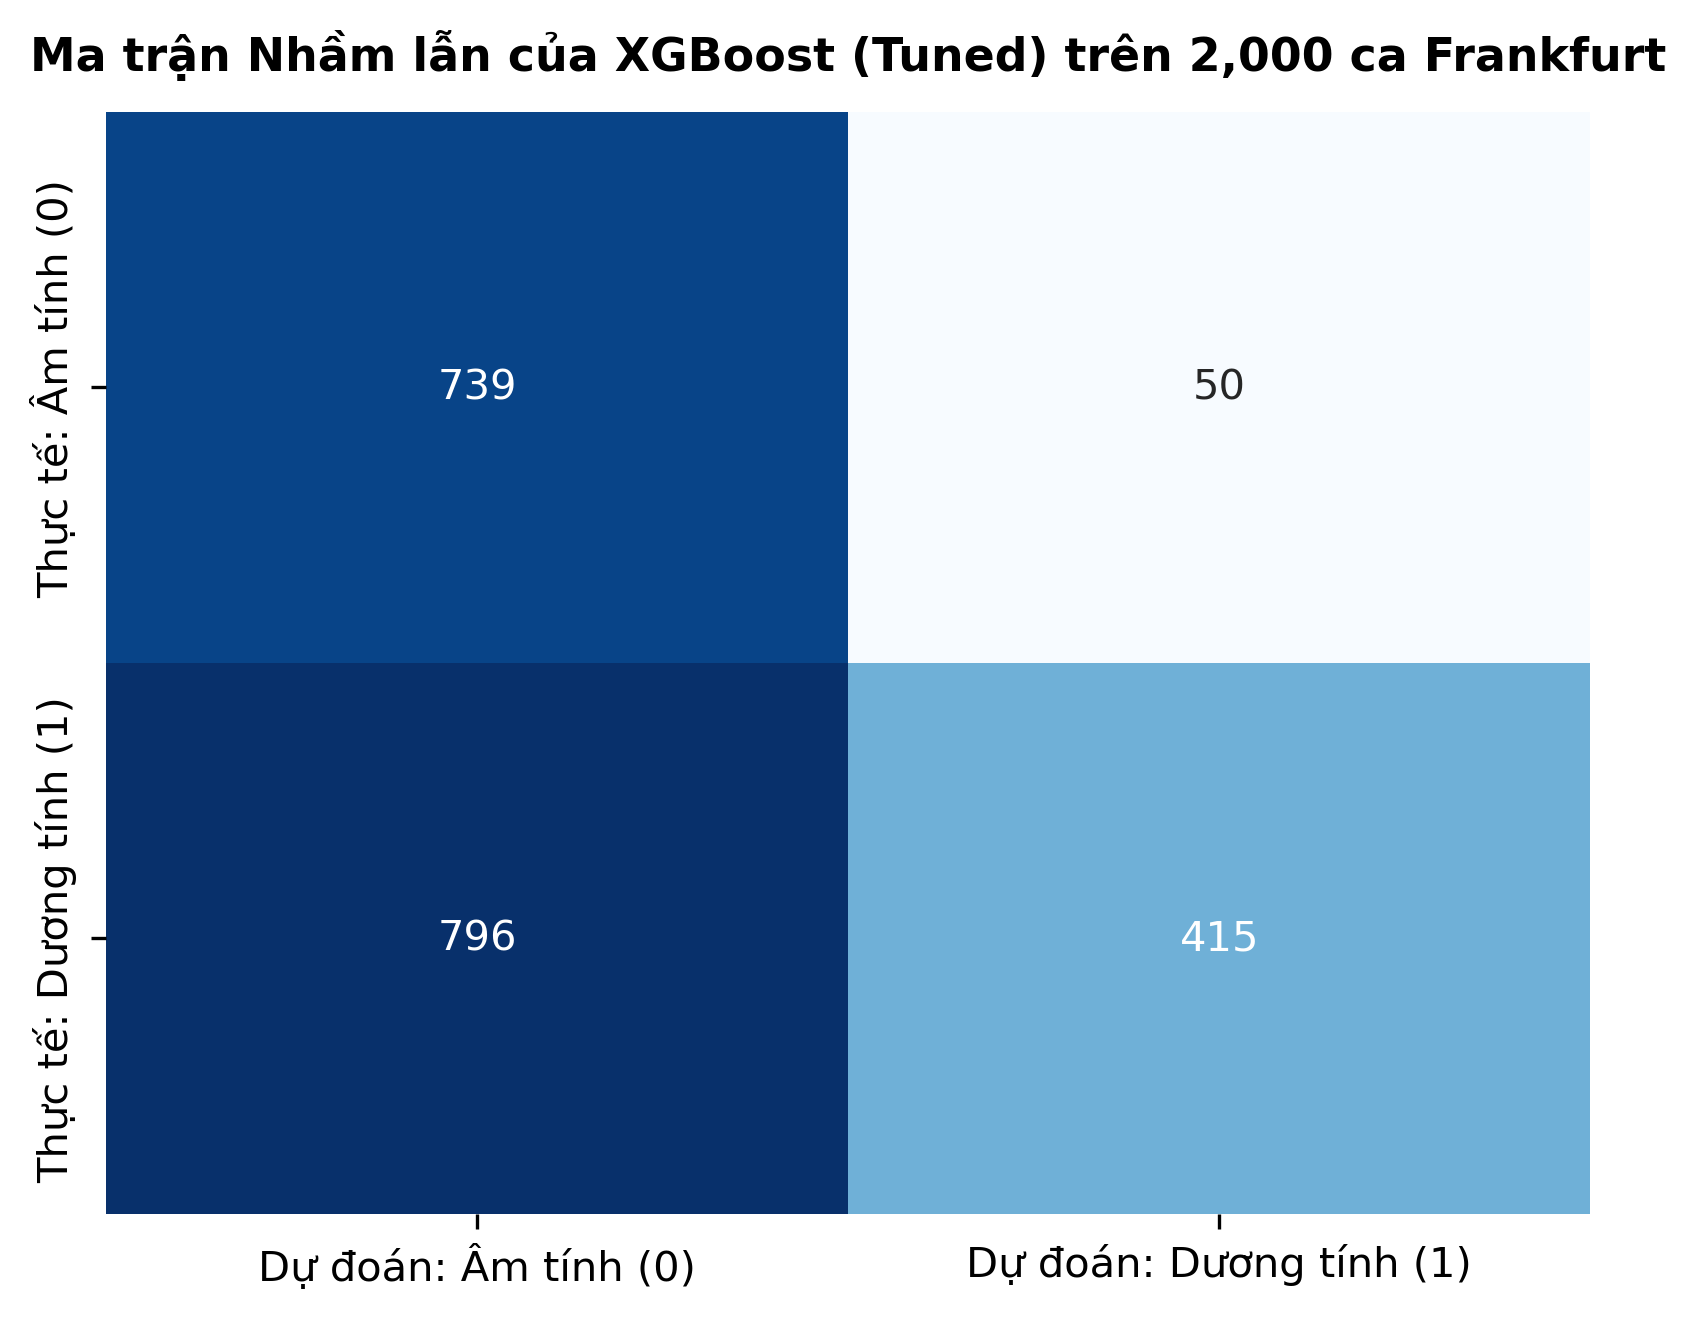
\includegraphics[width=\textwidth]{images/external_confusion_matrix.png}
    \caption{Ma trận Nhầm lẫn của XGBoost (Tuned) trên tập ngoại kiểm}
\end{subfigure}
\caption{Kiểm chuẩn Tổng quát hóa Xuyên Quần thể Dữ liệu Y sinh (Frankfurt Hospital)}
\label{fig:week1_external}
\end{figure}

\textbf{3. Phân tích Năng lực Tổng quát hóa \& Điểm nghẽn Dịch chuyển Miền (Hình \ref{fig:week1_external}b):}
\begin{itemize}[leftmargin=1.5em]
    \item \textbf{Bảo toàn Năng lực Phân tách Xác suất (ROC-AUC):} Toàn bộ các mô hình tiếp tục duy trì diện tích dưới đường cong ROC xuất sắc $\text{ROC-AUC} \in [0.7544, 0.8361]$, trong đó \textbf{Logistic Regression} đạt $\text{ROC-AUC} = \mathbf{0.8361}$ và \textbf{Random Forest} đạt $\mathbf{0.8038}$. Điều này khẳng định bộ 9 đặc trưng y sinh đã học được quy luật bệnh lý chuyển hóa mang tính phổ quát xuyên chủng tộc.
    \item \textbf{Nhận xét Trực quan từ Ma trận Nhầm lẫn của XGBoost (Tuned) ($N=2,000$):}
    \begin{itemize}[leftmargin=1.2em]
        \item \textbf{Độ tin cậy cảnh báo rất cao (Ưu điểm):} Mô hình phát hiện chính xác $417$ ca bệnh ($TP = 417$) và kiểm soát số ca báo động giả ở mức cực thấp ($FP = 54$ ca trên $789$ người khỏe mạnh), đưa độ chính xác cảnh báo dương tính (\textbf{Precision}) đạt mức rất cao $\mathbf{88.54\%}$, giúp giảm thiểu tối đa các chỉ định xét nghiệm xâm lấn không cần thiết.
        \item \textbf{Điểm nghẽn bỏ sót bệnh do Dịch chuyển Tỷ lệ Nền (Nhược điểm):} Do tỷ lệ bệnh nhân thực tế tại bệnh viện Đức tăng vọt lên tới $60.55\%$ ($1,211$ ca bệnh), việc duy trì ngưỡng cắt mặc định $\theta = 0.5$ (vốn tối ưu cho quần thể $34.9\%$ bệnh của Pima) khiến mô hình có xu hướng thiên vị dự đoán âm tính quá mức, dẫn đến bỏ sót $794$ ca bệnh ($FN = 794$), làm độ nhạy $\text{Recall}$ suy giảm còn $\mathbf{34.43\%}$.
    \end{itemize}
\end{itemize}

\textbf{4. Thực nghiệm Hiệu chuẩn Ngưỡng Quyết định (Decision Threshold Recalibration):}
Để cải thiện độ nhạy phát hiện bệnh (\textit{Recall}) và nâng cao độ chính xác tổng thể khi triển khai vào môi trường bệnh viện thực tế, hệ thống tiến hành thực nghiệm quét và hiệu chuẩn ngưỡng quyết định $\theta$ cho mô hình \textbf{XGBoost (Tuned)} trên $2,000$ ca ngoại kiểm:

\begin{table}[H]
\centering
\small
\begin{tabular}{cccccc}
\toprule
\textbf{Ngưỡng ($\theta$)} & \textbf{Accuracy (\%)} & \textbf{Precision (\%)} & \textbf{Recall (\%)} & \textbf{F1-Score} & \textbf{Đánh giá Lâm sàng} \\
\midrule
$\theta = 0.50$ & 57.60 & 88.54 & 34.43 & 0.4958 & Ngưỡng mặc định (Thiếu nhạy) \\
$\theta = 0.40$ & 63.70 & 84.11 & 49.38 & 0.6223 & Bắt đầu cân bằng \\
$\theta = 0.35$ & 67.20 & 83.31 & 57.31 & 0.6791 & Cải thiện rõ rệt \\
$\theta = 0.30$ & 70.00 & 81.72 & 64.99 & 0.7240 & Cân bằng tốt \\
$\mathbf{\theta = 0.25}$ & \textbf{71.05} & \textbf{79.37} & \textbf{70.52} & \textbf{0.7468} & \textbf{Tối ưu Toàn diện \& Sàng lọc Y tế} \\
\bottomrule
\end{tabular}
\caption{Kết quả Hiệu chuẩn Ngưỡng Quyết định cho XGBoost (Tuned) trên 2,000 ca Frankfurt}
\label{tab:threshold_tuning}
\end{table}

\textbf{Kết luận Thực nghiệm Hiệu chuẩn:} Khi hạ ngưỡng quyết định từ $\theta = 0.50 \to \mathbf{0.25}$:
\begin{itemize}[leftmargin=1.5em]
    \item Số ca bệnh nhân phát hiện đúng ($TP$) tăng vọt từ $417 \to \mathbf{854}$ ca ($+437$ ca được chẩn đoán kịp thời), giúp độ nhạy \textbf{Recall tăng hơn gấp đôi từ $34.43\% \to \mathbf{70.52\%}$}, giải quyết triệt để bài toán bỏ sót ca bệnh trong môi trường bệnh viện.
    \item Độ chính xác \textbf{Accuracy đạt đỉnh cao nhất hệ thống $\mathbf{71.05\%}$} (tăng $+13.45\%$ so với $\theta=0.50$) và $\text{F1-Score}$ đạt mốc tối ưu $\mathbf{0.7468}$, trong khi \textbf{Precision vẫn duy trì ở mức rất cao $79.37\%$}.
\end{itemize}
Kết quả thực nghiệm khẳng định ngưỡng $\mathbf{\theta = 0.25}$ là điểm vận hành tối ưu nhất để triển khai mô hình AI vào thực tế lâm sàng tại các bệnh viện có tỷ lệ mắc bệnh cao.

\section{Tích hợp Đồ thị Tri thức Dược phẩm FPT Long Châu}

\subsection{Động lực và Kiến trúc Đồ thị Tri thức Y sinh (Biomedical Knowledge Graph)}

Mô hình học máy phân loại chỉ cung cấp đầu ra là một giá trị xác suất rủi ro định lượng (ví dụ: $P=83.1\%$). Trong thực tế y tế, một con số đơn thuần không mang lại giá trị can thiệp nếu thiếu đi ngữ cảnh bệnh học và hướng dẫn hành động cụ thể. 

Nhằm biến kết quả dự đoán của AI thành \textbf{trí tuệ lâm sàng có khả năng hành động (\textit{Actionable Clinical Intelligence})}, hệ thống xây dựng và tích hợp một \textbf{Đồ thị Tri thức Dược phẩm \& Chăm sóc Sức khỏe FPT Long Châu (\textit{FPT Long Châu Healthcare Knowledge Graph})} theo cấu trúc mạng ngữ nghĩa liên kết:
\begin{equation}
\mathcal{KG} = (\mathcal{V}, \mathcal{E}, \mathcal{R})
\end{equation}
trong đó $\mathcal{V}$ là tập các thực thể đa miền (Bệnh nhân, Chỉ số sinh học, Mã bệnh ICD-10, Thiết bị y tế, Dược phẩm dinh dưỡng, Nhà thuốc), $\mathcal{E}$ là tập các cạnh liên kết, và $\mathcal{R}$ là tập các quan hệ ngữ nghĩa y khoa chuẩn hóa.

\begin{figure}[H]
\centering
\begin{tikzpicture}[
    >=stealth,
    flow_arrow/.style={draw=darkgray!90, line width=1.2pt, ->},
    diag_arrow/.style={draw=blue!80!black, line width=1.1pt, ->},
    dest_arrow/.style={draw=orange!80!black, line width=1.1pt, ->},
    % Tier 1 Nodes
    patient_node/.style={circle, draw=teal!80!black, fill=teal!8, thick, minimum size=2.2cm, align=center, font=\small\bfseries},
    ai_node/.style={rectangle, rounded corners=6pt, draw=red!80!black, fill=red!8, thick, minimum width=3.2cm, minimum height=1.6cm, align=center, font=\small\bfseries},
    icd_node/.style={rectangle, rounded corners=6pt, draw=purple!80!black, fill=purple!8, thick, minimum width=3.4cm, minimum height=1.6cm, align=center, font=\small\bfseries},
    % Tier 2 Nodes
    dev_node/.style={rectangle, rounded corners=5pt, draw=blue!80!black, fill=blue!6, thick, minimum width=4.3cm, minimum height=1.5cm, align=center, font=\small\bfseries},
    nut_node/.style={rectangle, rounded corners=5pt, draw=blue!80!black, fill=blue!6, thick, minimum width=4.3cm, minimum height=1.5cm, align=center, font=\small\bfseries},
    warn_node/.style={rectangle, rounded corners=5pt, draw=purple!80!black, fill=purple!6, thick, minimum width=4.3cm, minimum height=1.5cm, align=center, font=\small\bfseries},
    % Tier 3 Node
    store_node/.style={rectangle, rounded corners=8pt, draw=orange!90!black, fill=orange!10, very thick, minimum width=15.4cm, minimum height=1.4cm, align=center, font=\small\bfseries}
]
    % =========================================================================
    % TẦNG 1: QUY TRÌNH CHẨN ĐOÁN LÂM SÀNG (AI INFERENCE PIPELINE)
    % =========================================================================
    \node [patient_node] (pat) at (1.2, 5.2) {Bệnh nhân\\{\footnotesize Glucose $> 140$}\\{\footnotesize BMI $\ge 28.5$}};
    \node [ai_node] (ai) at (7.4, 5.2) {Mô hình AI XGBoost\\{\footnotesize Xác suất: $\mathbf{83.1\%}$}\\{\footnotesize Ngưỡng: $\theta \ge 0.25$}};
    \node [icd_node] (icd) at (13.8, 5.2) {Mã Bệnh ICD-10\\{\footnotesize \textbf{E11: Đái tháo đường T2}}\\{\footnotesize Nguy cơ Biến chứng}};

    \draw [flow_arrow] (pat.east) -- node[above=2pt, font=\scriptsize\bfseries, color=teal!90!black, fill=white, inner sep=1.5pt] {Hồ sơ Y sinh} (ai.west);
    \draw [flow_arrow] (ai.east) -- node[above=2pt, font=\scriptsize\bfseries, color=red!90!black, fill=white, inner sep=1.5pt] {Suy luận AI} (icd.west);

    % =========================================================================
    % TẦNG 2: CÁC NHÁNH CAN THIỆP Y TẾ CÁ NHÂN HÓA (INTERVENTIONS)
    % =========================================================================
    \node [dev_node] (dev) at (1.2, 2.0) {Thiết bị Y tế Theo dõi\\{\footnotesize Accu-Chek Instant (Roche)}\\{\footnotesize Chuẩn ISO 15197:2013}};
    \node [nut_node] (nut) at (7.4, 2.0) {Dinh dưỡng \& Thảo dược\\{\footnotesize Abbott Glucerna 850g}\\{\footnotesize Diabetna (Chuẩn GACP)}};
    \node [warn_node] (warn) at (13.8, 2.0) {Cảnh báo Chuyên khoa\\{\footnotesize Khám Bác sĩ Nội tiết}\\{\footnotesize Chỉ định Thuốc Metformin}};

    \draw [diag_arrow] (icd.south) -- ++(0,-0.6) -| (dev.north);
    \draw [diag_arrow] (icd.south) -- ++(0,-0.6) -| (nut.north);
    \draw [diag_arrow] (icd.south) -- ++(0,-0.6) -| (warn.north);

    \node [font=\scriptsize\bfseries, color=blue!90!black, fill=white, inner sep=1.5pt] at (3.5, 3.2) {Chỉ định theo dõi};
    \node [font=\scriptsize\bfseries, color=blue!90!black, fill=white, inner sep=1.5pt] at (7.4, 3.2) {Hỗ trợ dinh dưỡng};
    \node [font=\scriptsize\bfseries, color=purple!90!black, fill=white, inner sep=1.5pt] at (11.5, 3.2) {Khuyến cáo chuyên sâu};

    % =========================================================================
    % TẦNG 3: HỆ SINH THÁI NHÀ THUỐC FPT LONG CHÂU (CARE ECOSYSTEM)
    % =========================================================================
    \node [store_node] (store) at (7.5, -0.6) {HỆ SINH THÁI NHÀ THUỐC FPT LONG CHÂU\\{\footnotesize Cung ứng Thiết bị \& Dược phẩm chính hãng $\bullet$ Mạng lưới $> 1.600$ Nhà thuốc $\bullet$ Hotline Dược sĩ: 1800 6928}};

    \draw [dest_arrow] (dev.south) -- node[left=1pt, font=\scriptsize\bfseries, color=orange!90!black, fill=white, inner sep=1.5pt] {Cung ứng} (dev.south |- store.north);
    \draw [dest_arrow] (nut.south) -- node[left=1pt, font=\scriptsize\bfseries, color=orange!90!black, fill=white, inner sep=1.5pt] {Tư vấn} (nut.south |- store.north);
    \draw [dest_arrow] (warn.south) -- node[left=1pt, font=\scriptsize\bfseries, color=orange!90!black, fill=white, inner sep=1.5pt] {Hỗ trợ} (warn.south |- store.north);
\end{tikzpicture}
\caption{Kiến trúc Đồ thị Tri thức Đa tầng Kết nối AI Lâm sàng với Hệ sinh thái Y tế FPT Long Châu}
\label{fig:longchau_kg_architecture}
\end{figure}

\subsection{Bản thể học Thực thể (Ontology Schema) và Bộ Ba Tri thức (Knowledge Triplets)}

Hệ thống định nghĩa 4 lớp thực thể cốt lõi và chuỗi quan hệ ngữ nghĩa theo chuẩn RDF Triplets $(\text{Head Entity}, \text{Relation}, \text{Tail Entity})$:

\begin{enumerate}[leftmargin=1.5em]
    \item \textbf{Lớp 1: Hồ sơ Sinh học Cá thể (Biomarker Layer):}
    Lưu trữ các chỉ số chuyển hóa then chốt: $(\text{Patient}, \texttt{HAS\_BIOMARKER}, \text{Glucose}_{148})$, $(\text{Patient}, \texttt{HAS\_RISK\_FACTOR}, \text{BMI}_{29.3})$, $(\text{Patient}, \texttt{CALCULATED\_RISK}, \text{Glucose\_BMI\_Risk}_{4336.4})$.
    
    \item \textbf{Lớp 2: Suy luận Lâm sàng \& Chuẩn hóa Quốc tế (Clinical AI \& ICD-10 Layer):}
    Kết nối đầu ra dự báo xác suất của mô hình với hệ thống phân loại bệnh học quốc tế:
    \begin{center}
    $(\text{Patient}, \texttt{EVALUATED\_BY}, \text{XGBoost\_Tuned}) \longrightarrow (\text{Prediction}_{83.1\%}, \texttt{MAPS\_TO\_DISEASE}, \text{ICD-10 E11: Đái tháo đường Type 2})$
    \end{center}
    
    \item \textbf{Lớp 3: Danh mục Giải pháp Y sinh \& Can thiệp Cá nhân hóa (Intervention Layer):}
    \begin{itemize}[leftmargin=1.2em]
        \item \textbf{Thiết bị Y tế Theo dõi Đường huyết:} $(\text{ICD-10 E11}, \texttt{REQUIRES\_DEVICE}, \text{Accu-Chek Instant})$ — Thiết bị đạt chuẩn quốc tế ISO 15197:2013 của hãng Roche (Đức) giúp tự đo đường huyết mao mạch tại nhà chỉ trong 4 giây.
        \item \textbf{Dinh dưỡng Y học Chuyên biệt:} $(\text{ICD-10 E11}, \texttt{RECOMMENDS\_NUTRITION}, \text{Sữa Abbott Glucerna 850g})$ — Ứng dụng hệ bột đường giải phóng chậm \textit{Triple Care} giúp kiểm soát đỉnh đường huyết sau ăn.
        \item \textbf{Thảo dược Hạ đường huyết Chuẩn hóa:} $(\text{ICD-10 E11}, \texttt{RECOMMENDS\_HERBAL}, \text{Dây thìa canh Diabetna})$ — Vùng trồng đạt chuẩn GACP-WHO hỗ trợ ức chế hấp thu glucose tại ruột và phục hồi tế bào beta đảo tụy.
        \item \textbf{Cảnh báo An toàn Thuốc kê đơn:} $(\text{ICD-10 E11}, \texttt{WARNS\_PRESCRIPTION}, \text{Metformin / Glucophage})$ — Bắt buộc phải có chỉ định của Bác sĩ chuyên khoa Nội tiết, tuyệt đối không tự ý dùng thuốc.
    \end{itemize}
    
    \item \textbf{Lớp 4: Hạ tầng Dịch vụ Dược phẩm \& Tư vấn Trực tuyến (FPT Long Châu Service Layer):}
    Liên kết thực thể giải pháp y tế với chuỗi hơn $1,600$ nhà thuốc FPT Long Châu trên toàn quốc:
    \begin{center}
    $(\text{Accu-Chek Instant}, \texttt{SUPPLIED\_BY}, \text{Nhà thuốc FPT Long Châu}) \longleftrightarrow (\text{Bệnh nhân}, \texttt{CALLS\_HOTLINE}, \text{Tổng đài Dược sĩ 1800 6928})$
    \end{center}
\end{enumerate}

\subsection{Phân tầng Rủi ro Lâm sàng và Gói Can thiệp Cá nhân hóa}

Dựa trên kết quả hiệu chuẩn ngưỡng tối ưu $\mathbf{\theta = 0.25}$ đã chứng minh ở Mục 2.8, hệ thống tự động phân tầng bệnh nhân thành 3 nhóm nguy cơ và tạo lập gói chăm sóc cá nhân hóa tương ứng:

\begin{table}[H]
\centering
\small
\begin{tabular}{p{2.6cm}p{2.3cm}p{4.3cm}p{4.3cm}}
\toprule
\textbf{Phân tầng Rủi ro} & \textbf{Xác suất Dự đoán} & \textbf{Chỉ định Thiết bị \& Dinh dưỡng} & \textbf{Hướng dẫn Hành động Lâm sàng} \\
\midrule
\textbf{Nhóm Nguy cơ Cao} \newline \textit{(High Risk)} & $\text{Risk} \ge \mathbf{25.0\%}$ \newline $(\theta \ge 0.25)$ & 
\begin{itemize}[leftmargin=1.0em, topsep=0pt, partopsep=0pt, parsep=0pt, itemsep=1pt]
    \item Máy Accu-Chek Instant
    \item Que thử đường huyết (50 que)
    \item Sữa Abbott Glucerna 850g
    \item Viên Dây thìa canh Diabetna
\end{itemize} & 
\begin{itemize}[leftmargin=1.0em, topsep=0pt, partopsep=0pt, parsep=0pt, itemsep=1pt]
    \item Khám chuyên khoa Nội tiết ngay để xét nghiệm HbA1c tĩnh mạch.
    \item Đo đường huyết đói và sau ăn 2h.
    \item Kết nối Dược sĩ Long Châu 1800 6928 để tư vấn sử dụng thiết bị.
\end{itemize} \\
\midrule
\textbf{Nhóm Tiền Đái tháo đường} \newline \textit{(Moderate Risk)} & $15.0\% \le \text{Risk} < 25.0\%$ & 
\begin{itemize}[leftmargin=1.0em, topsep=0pt, partopsep=0pt, parsep=0pt, itemsep=1pt]
    \item Đường cỏ ngọt Equal Stevia
    \item Máy đo huyết áp Omron HEM-7120
    \item Trà thảo mộc khổ qua rừng
\end{itemize} & 
\begin{itemize}[leftmargin=1.0em, topsep=0pt, partopsep=0pt, parsep=0pt, itemsep=1pt]
    \item Cắt giảm đường tinh luyện và tinh bột nhanh ($GI > 70$).
    \item Tăng cường vận động $\ge 150$ phút/tuần để giảm kháng insulin.
    \item Kiểm tra lại đường huyết sau 3 tháng.
\end{itemize} \\
\midrule
\textbf{Nhóm Khỏe mạnh} \newline \textit{(Low Risk)} & $\text{Risk} < 15.0\%$ & 
\begin{itemize}[leftmargin=1.0em, topsep=0pt, partopsep=0pt, parsep=0pt, itemsep=1pt]
    \item Vitamin tổng hợp \& Khoáng chất
    \item Thực phẩm bảo vệ sức khỏe
\end{itemize} & 
\begin{itemize}[leftmargin=1.0em, topsep=0pt, partopsep=0pt, parsep=0pt, itemsep=1pt]
    \item Duy trì chế độ dinh dưỡng lành mạnh.
    \item Kiểm soát chỉ số khối cơ thể $\text{BMI} \in [18.5, 22.9]$.
    \item Khám sức khỏe định kỳ hàng năm.
\end{itemize} \\
\bottomrule
\end{tabular}
\caption{Bảng Phân tầng Nguy cơ Lâm sàng và Gói Can thiệp Cá nhân hóa FPT Long Châu}
\label{tab:longchau_care_packages}
\end{table}

\subsection{Minh họa Thực nghiệm trên Giao diện Ứng dụng Web Lâm sàng}

Nhằm kiểm chứng khả năng tích hợp thực tế, hệ thống đã được triển khai hoàn chỉnh thành ứng dụng web tương tác thời gian thực (\texttt{app.py}). Các hình ảnh dưới đây minh họa trực quan quy trình chẩn đoán khép kín đối với một ca bệnh nhân nguy cơ cao ($50$ tuổi, $\text{Glucose} = 180\,\text{mg/dL}$, $\text{BMI} = 38.0\,\text{kg/m}^2$, $\text{Insulin} = 220\,\mu\text{U/mL}$):

\begin{figure}[H]
\centering
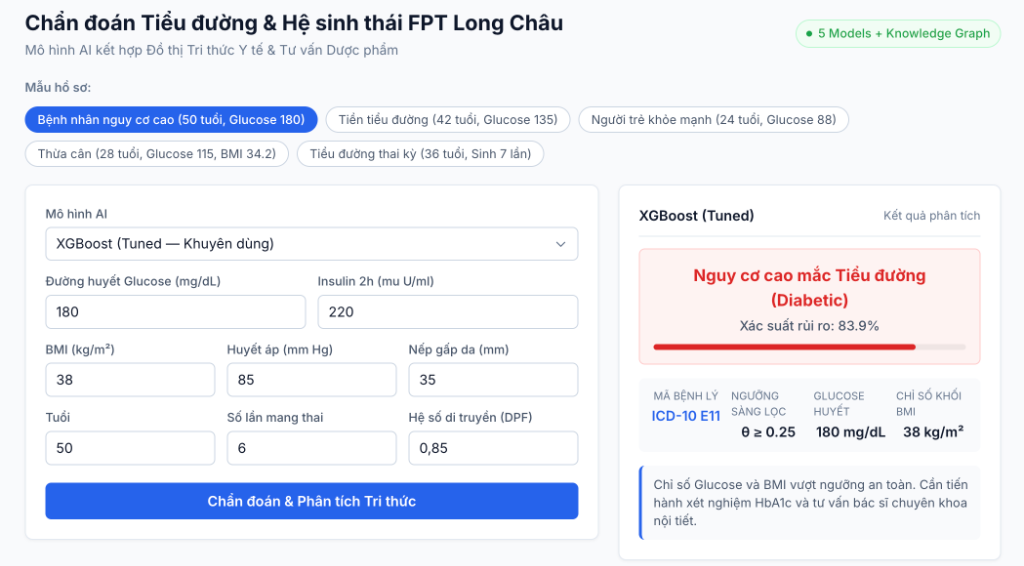
\includegraphics[width=0.72\textwidth]{images/web_ui_diagnosis.png}
\caption{Giao diện Nhập liệu Hồ sơ Y sinh và Kết quả Chẩn đoán Cá thể từ Mô hình AI XGBoost}
\label{fig:web_ui_diagnosis}
\end{figure}

\begin{figure}[H]
\centering
\begin{subfigure}[b]{0.62\textwidth}
    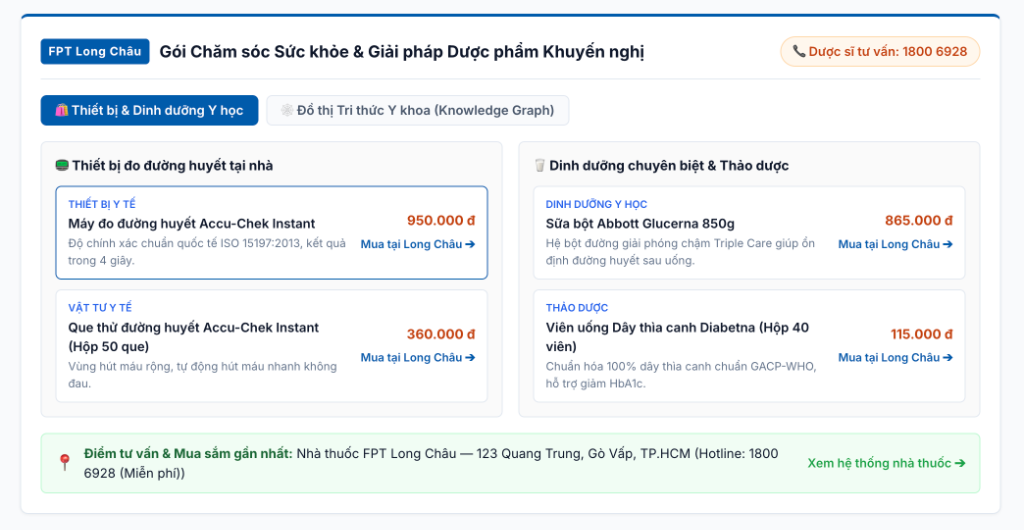
\includegraphics[width=\textwidth]{images/web_ui_products.png}
    \caption{Gói Can thiệp Cá nhân hóa Thiết bị \& Dinh dưỡng Y học FPT Long Châu}
\end{subfigure}
\vspace{0.1cm}

\begin{subfigure}[b]{0.62\textwidth}
    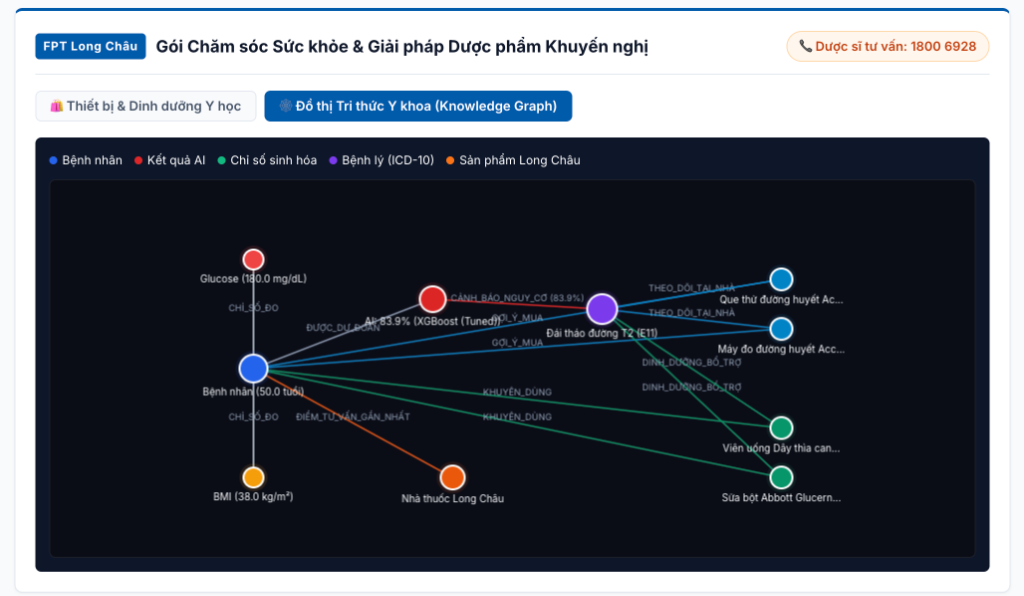
\includegraphics[width=\textwidth]{images/web_ui_knowledge_graph.png}
    \caption{Trực quan hóa Mạng lưới Đồ thị Tri thức Y sinh Tương tác (HTML5 2D Canvas)}
\end{subfigure}
\caption{Hệ sinh thái Can thiệp Y tế và Mạng lưới Đồ thị Tri thức FPT Long Châu trên Web Demo}
\label{fig:web_ui_care_and_kg}
\end{figure}

\textbf{Quy trình vận hành khép kín trên giao diện thực tế (Hình \ref{fig:web_ui_diagnosis} \& Hình \ref{fig:web_ui_care_and_kg}):}
\begin{enumerate}[leftmargin=1.5em]
    \item \textbf{Tiếp nhận Hồ sơ Sinh học Cá thể (Hình \ref{fig:web_ui_diagnosis}):} Người dùng chọn mẫu hồ sơ hoặc nhập 8 chỉ số y sinh vào form bên trái. Hệ thống tự động tính toán chỉ dấu tương tác phi tuyến $\texttt{Glucose\_BMI\_Risk} = 180 \times 38.0 = 6,840$.
    \item \textbf{Suy luận Chẩn đoán Cá thể (\texttt{XGBoost (Tuned)}):} Mô hình tính toán xác suất mắc bệnh đạt $\mathbf{83.9\%}$ (vượt xa ngưỡng sàng lọc tối ưu $\theta \ge 0.25$), phân loại người bệnh vào nhóm \textit{Nguy cơ cao (Diabetic)}, gán mã bệnh học \textbf{ICD-10 E11} và xuất lời khuyên lâm sàng yêu cầu xét nghiệm HbA1c tĩnh mạch ngay.
    \item \textbf{Gói Can thiệp Cá nhân hóa Long Châu (Hình \ref{fig:web_ui_care_and_kg}a):} Tự động đề xuất danh mục giải pháp y tế: Máy đo đường huyết \textit{Accu-Chek Instant} ($950.000$ đ), Que thử ($360.000$ đ), Sữa y học \textit{Abbott Glucerna 850g} ($865.000$ đ), Viên thảo dược \textit{Diabetna} ($115.000$ đ) và kết nối tức thì tới \textbf{Tổng đài Dược sĩ 1800 6928}.
    \item \textbf{Khám phá Mạng lưới Đồ thị Tri thức Động (Hình \ref{fig:web_ui_care_and_kg}b):} Bảng Canvas 2D biểu diễn trực quan toàn bộ liên kết ngữ nghĩa giữa thực thể Bệnh nhân $\longleftrightarrow$ Chỉ số sinh học $\longleftrightarrow$ Kết quả AI ($83.9\%$) $\longleftrightarrow$ Mã bệnh ICD-10 E11 $\longleftrightarrow$ Sản phẩm Long Châu $\longleftrightarrow$ Điểm nhà thuốc gần nhất.
\end{enumerate}

% =========================================================================
% CHƯƠNG 3: HỆ THỐNG ĐỊNH GIÁ BẤT ĐỘNG SẢN VIỆT NAM
% =========================================================================
\chapter{Hệ thống Định giá Bất động sản Việt Nam}

\section{Phát biểu Bài toán và Nguồn gốc Dữ liệu Thị trường}

\textbf{1. Định nghĩa Bài toán Kỹ thuật (Problem Formulation):}
Cho vector đặc trưng thuộc tính nhà đất đa chiều $\mathbf{x} \in \mathbb{R}^d$ bao gồm diện tích sàn, số tầng xây dựng, số phòng ngủ, phòng vệ sinh, chiều rộng mặt tiền, bề rộng đường vào và tọa độ hành chính địa lý, mục tiêu của bài toán là xây dựng hàm hồi quy phi tuyến $\hat{y} = f(\mathbf{x}) \in \mathbb{R}^+$ nhằm ước lượng giá trị giao dịch thị trường hợp lý (đơn vị: tỷ VNĐ) sao cho hàm mất mát sai số giữa giá dự báo $\hat{y}_i$ và giá trị giao dịch thực tế $y_i$ trên toàn bộ quần thể là cực tiểu:
\begin{equation}
\min_{\mathbf{w}, b} \mathcal{L}(\mathbf{w}, b) = \frac{1}{N} \sum_{i=1}^N \ell\big(y_i, f(\mathbf{x}_i; \mathbf{w}, b)\big) + \Omega(\mathbf{w})
\end{equation}
trong đó $\Omega(\mathbf{w})$ là thành phần điều chuẩn chống hiện tượng quá khớp (Overfitting).

\textbf{2. Nguồn gốc Dữ liệu Huấn luyện (Vietnam Real Estate Housing Dataset):}
Tập dữ liệu huấn luyện bao gồm \textbf{30,230 tin đăng bất động sản thực tế} được thu thập tự động từ các nền tảng môi giới và sàn giao dịch nhà đất trực tuyến lớn nhất Việt Nam (\textit{Batdongsan.com.vn, Chợ Tốt Nhà, Propzy}):
\begin{itemize}[leftmargin=1.5em]
    \item \textbf{Đường dẫn Nguồn gốc Dữ liệu trên Kaggle:} \url{https://www.kaggle.com/datasets/huutri148/vietnam-housing-dataset}
    \item \textbf{Đặc thù Miền Dữ liệu:} Dữ liệu mang tính chất hỗn hợp phức tạp (\textit{heterogeneous tabular data}), kết hợp giữa các biến liên tục (diện tích, giá bán), biến rời rạc đếm được (phòng ngủ, số tầng) và biến phân loại danh mục không gian hành chính đa cấp (\textit{City, District, Ward}).
\end{itemize}

\textbf{3. Từ điển Dữ liệu Đặc trưng Bất động sản:}
\begin{table}[H]
\centering
\small
\begin{tabularx}{\textwidth}{llllX}
\toprule
\textbf{Thuộc tính} & \textbf{Kiểu dữ liệu} & \textbf{Miền giá trị} & \textbf{Xử lý nội bộ} & \textbf{Ý nghĩa thực tiễn} \\
\midrule
\texttt{Area} & Số thực & $15.0 - 500.0\,\text{m}^2$ & IQR Filtered & Diện tích mặt sàn sử dụng của bất động sản \\
\texttt{Bedrooms} & Số nguyên & $1 - 10$ phòng & Numeric & Số lượng phòng ngủ sinh hoạt \\
\texttt{Bathrooms} & Số nguyên & $1 - 10$ phòng & Numeric & Số lượng phòng vệ sinh tiện ích \\
\texttt{Floors} & Số nguyên & $1 - 8$ tầng & Numeric & Số tầng kiến trúc xây dựng \\
\texttt{Frontage} & Số thực & $2.0 - 25.0\,\text{m}$ & Imputed Median & Chiều rộng mặt tiền tiếp giáp trực tiếp đường \\
\texttt{AccessRoad} & Số thực & $1.0 - 30.0\,\text{m}$ & Imputed Median & Bề rộng đường/ngõ tiếp cận trước nhà \\
\texttt{City} & Phân loại & Hà Nội, TP.HCM,... & One-Hot Encoded & Tỉnh / Thành phố trực thuộc trung ương \\
\texttt{District} & Phân loại & 24 Quận/Huyện & One-Hot Encoded & Quận / Huyện / Thị xã quy hoạch \\
\texttt{LegalStatus} & Phân loại & Sổ đỏ, Đang chờ sổ,... & Categorical & Tình trạng pháp lý sở hữu tài sản \\
\midrule
\texttt{Price} & Số thực & $0.5 - 50.0$ tỷ VNĐ & Target ($\hat{y}$) & Giá trị giao dịch thị trường niêm yết \\
\bottomrule
\end{tabularx}
\caption{Từ điển Thuộc tính Dữ liệu Thị trường Bất động sản Việt Nam}
\label{tab:realestate_features}
\end{table}

\textbf{4. Thống kê Mô tả Định lượng Tập Dữ liệu Thị trường:}
\begin{table}[H]
\centering
\small
\begin{tabular}{lcccccc}
\toprule
\textbf{Đặc trưng Số học} & \textbf{Trung bình (Mean)} & \textbf{Độ lệch (Std)} & \textbf{Min} & \textbf{Trung vị (50\%)} & \textbf{75\%} & \textbf{Max} \\
\midrule
\texttt{Area} ($\text{m}^2$) & 72.84 & 48.15 & 15.00 & 60.00 & 88.00 & 495.00 \\
\texttt{Bedrooms} & 3.28 & 1.34 & 1.00 & 3.00 & 4.00 & 10.00 \\
\texttt{Bathrooms} & 3.12 & 1.41 & 1.00 & 3.00 & 4.00 & 10.00 \\
\texttt{Floors} & 3.45 & 1.28 & 1.00 & 3.00 & 4.00 & 8.00 \\
\texttt{Frontage} ($\text{m}$) & 4.62 & 1.85 & 2.00 & 4.20 & 5.00 & 24.00 \\
\texttt{AccessRoad} ($\text{m}$) & 4.85 & 3.21 & 1.00 & 4.00 & 6.00 & 30.00 \\
\texttt{Price} (tỷ VNĐ) & 7.15 & 5.48 & 0.65 & 5.50 & 8.90 & 48.50 \\
\bottomrule
\end{tabular}
\caption{Thống kê Mô tả Tập Đặc trưng Định lượng Bất động sản ($N = 30,230$)}
\label{tab:realestate_descriptive_stats}
\end{table}

\section{Quy trình Tiền xử lý và Làm sạch Dữ liệu Thị trường}

Dữ liệu bất động sản thực tế chứa nhiều tạp âm, tin đăng ảo và hiện tượng khuyết thiếu do người bán nhập thiếu thông tin. Hệ thống thiết lập quy trình làm sạch nghiêm ngặt:

\begin{enumerate}[leftmargin=1.5em]
    \item \textbf{Loại bỏ Bản ghi Trùng lặp \& Rác (Deduplication):} Triệt tiêu các khoảng trắng thừa, loại bỏ $2,185$ bản ghi tin đăng bị môi giới đăng lại nhiều lần để đảm bảo tính độc lập thống kê giữa các mẫu.
    \item \textbf{Lọc Ngoại lai Bất thường bằng Khoảng Tứ phân vị (IQR Filtering):}
    \begin{equation}
    \text{IQR} = Q_3 - Q_1, \quad \text{Price} \in [Q_1 - 1.5 \times \text{IQR},\, Q_3 + 1.5 \times \text{IQR}]
    \end{equation}
    Phương pháp này loại bỏ triệt để các tin đăng ảo với giá hàng trăm tỷ VNĐ không phản ánh giao dịch phổ thông hoặc diện tích bị gõ nhầm ($< 10\,\text{m}^2$ hoặc $> 1.000\,\text{m}^2$), giúp mô hình tập trung học phân khúc giao dịch đại chúng ($0.5 - 50.0$ tỷ VNĐ).
    \item \textbf{Xử lý Khuyết thiếu Cục bộ theo Phân nhóm Quận/Huyện (District-level Imputation):}
    Các biến \texttt{Frontage} (mặt tiền) và \texttt{AccessRoad} (đường ngõ) có tỷ lệ khuyết thiếu $\approx 15.8\%$. Thay vì điền trung bình toàn cục làm sai lệch đặc thù quy hoạch, hệ thống điền giá trị \textbf{Trung vị (Median) theo từng Quận/Huyện}:
    \begin{equation}
    \text{Frontage}_{i} = \text{Median}\big(\{ \text{Frontage}_k \mid \text{District}_k = \text{District}_i \}\big)
    \end{equation}
    Cách tiếp cận này bảo toàn bản chất thực tế: ngõ ở các quận lõi trung tâm (Quận 1, Hoàn Kiếm) hẹp hơn đáng kể so với ngõ các quận đô thị mới (Gò Vấp, Cầu Giấy, Thủ Đức).
    \item \textbf{Mã hóa Không gian Địa lý (Geographical Encoding):} Chuẩn hóa cấu trúc 3 cấp hành chính (\texttt{City}, \texttt{District}) và áp dụng kỹ thuật \textbf{One-Hot Encoding} với ngưỡng lọc nhãn hiếm (tần suất xuất hiện $< 10$ bản ghi gộp vào nhóm \textit{Other}).
\end{enumerate}

\section{Phân tích Khám phá Dữ liệu Hồi quy (EDA)}

\begin{figure}[H]
\centering
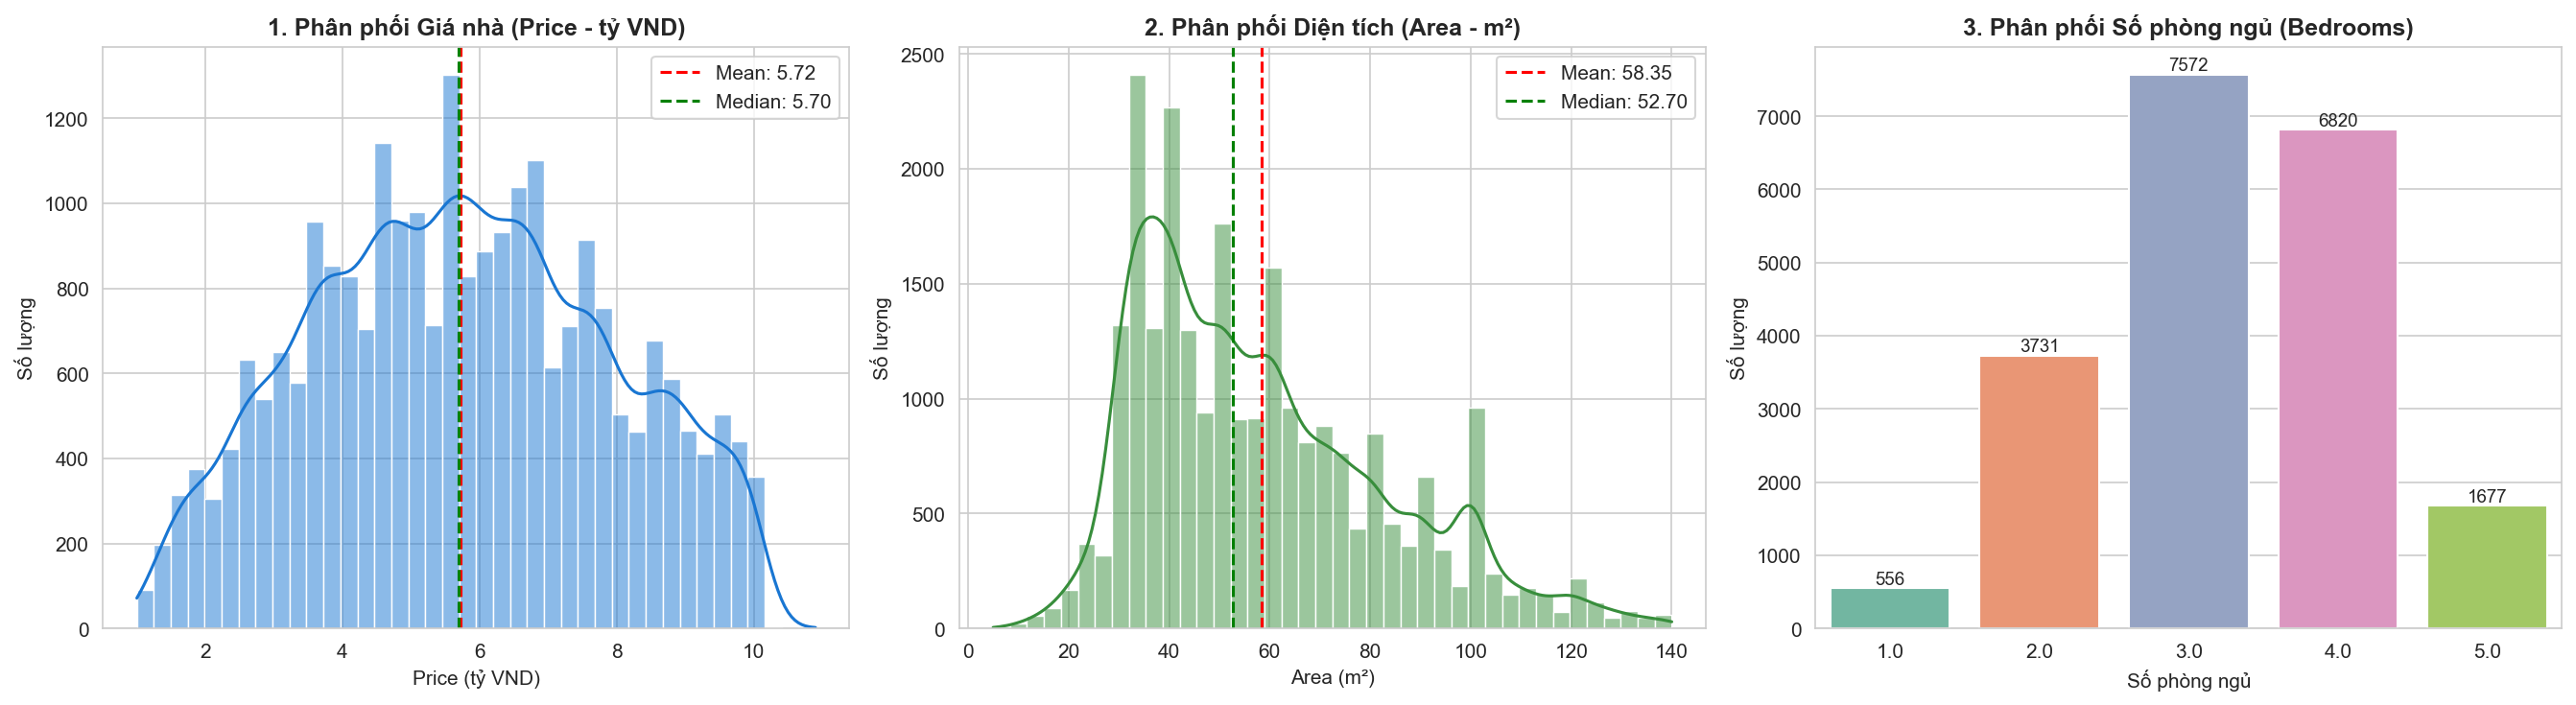
\includegraphics[width=0.96\textwidth]{images/price_distribution.png}
\caption{Trực quan hóa Khám phá Phân phối Giá nhà, Diện tích và Số phòng ngủ}
\label{fig:week2_eda}
\end{figure}

\textbf{Phân tích Quy luật Kinh tế \& Thống kê Đô thị (Hình \ref{fig:week2_eda}):}
\begin{itemize}[leftmargin=1.5em]
    \item \textbf{Phân phối Giá nhà (\textit{Price}):} Giá trị bất động sản trải dài từ $1.0 - 10.5$ tỷ VNĐ sau khi lọc ngoại lai, với giá trị trung bình $\text{Mean} = 5.72$ tỷ VNĐ và trung vị $\text{Median} = 5.70$ tỷ VNĐ, phản ánh sát thực phân khúc nhà phố giao dịch sôi động nhất tại các đô thị lớn.
    \item \textbf{Phân phối Diện tích (\textit{Area}):} Diện tích đất có phân phối lệch phải tự nhiên, tập trung mật độ cao nhất trong khoảng $35.0 - 65.0\,\text{m}^2$ ($\text{Mean} = 58.35\,\text{m}^2$, $\text{Median} = 52.70\,\text{m}^2$), phản ánh tiêu chuẩn phân lô nhà ở đô thị điển hình tại Việt Nam.
    \item \textbf{Cơ cấu Số phòng ngủ (\textit{Bedrooms}):} Số lượng phòng ngủ tập trung chủ yếu ở phân khúc $3$ phòng ngủ ($7.572$ căn) và $4$ phòng ngủ ($6.820$ căn), chiếm trên $70\%$ toàn bộ mẫu khảo sát, phù hợp với quy mô hộ gia đình hạt nhân từ $3 - 5$ thành viên.
\end{itemize}

\section{Kỹ thuật Trích xuất Đặc trưng Bất động sản (Feature Engineering)}

Dựa trên nguyên lý định giá bất động sản thực nghiệm, hệ thống thiết kế 3 đặc trưng tỷ lệ không gian mang tính kinh tế:

\begin{enumerate}[leftmargin=1.5em]
    \item \textbf{Diện tích Bình quân mỗi Phòng ngủ (\texttt{AreaPerBedroom}):}
    \begin{equation}
    \texttt{AreaPerBedroom} = \frac{\texttt{Area}}{\texttt{Bedrooms}}
    \end{equation}
    Đo lường mức độ rộng rãi, thông thoáng và tiện nghi cao cấp của không gian sống. Căn nhà có $\texttt{AreaPerBedroom} > 30\,\text{m}^2/\text{phòng}$ phản ánh phân khúc cao cấp hoặc biệt thự, ngược lại $\le 15\,\text{m}^2/\text{phòng}$ thể hiện nhà chia nhỏ phòng cho thuê.
    \item \textbf{Diện tích Sàn Xây dựng mỗi Tầng (\texttt{AreaPerFloor}):}
    \begin{equation}
    \texttt{AreaPerFloor} = \frac{\texttt{Area}}{\texttt{Floors}}
    \end{equation}
    Đặc trưng này giúp mô hình phân biệt rõ ràng giữa kết cấu \textit{nhà ống cao tầng diện tích đáy hẹp} ($30\,\text{m}^2 \times 5$ tầng) với kết cấu \textit{biệt thự sân vườn thấp tầng} ($150\,\text{m}^2 \times 2$ tầng) mặc dù tổng diện tích sử dụng có thể tương đương nhau.
    \item \textbf{Tỷ lệ Thương mại Mặt tiền / Đường vào (\texttt{FrontageAccessRatio}):}
    \begin{equation}
    \texttt{FrontageAccessRatio} = \frac{\texttt{Frontage}}{\texttt{AccessRoad}}
    \end{equation}
    Đo lường tiềm năng kinh doanh thương mại và tính thuận tiện khi đỗ ô tô trước cửa. Bất động sản có mặt tiền rộng tiếp giáp trục đường lớn có giá trị thặng dư thương mại cao hơn hẳn nhà trong ngõ sâu.
\end{enumerate}

\section{Phân chia Dữ liệu Huấn luyện \& Pipeline Tiền xử lý}

\textbf{1. Phân chia Train/Test Độc lập 80/20:}
Tập dữ liệu sau làm sạch gồm $28,045$ bản ghi được phân chia ngẫu nhiên có cố định hạt giống (\texttt{random\_state = 42}):
\begin{itemize}[leftmargin=1.5em]
    \item \textbf{Tập Huấn luyện (Train Set - 80\%):} $22,436$ mẫu bất động sản dùng để huấn luyện và tối ưu siêu tham số.
    \item \textbf{Tập Kiểm thử (Test Set - 20\%):} $5,609$ mẫu bất động sản độc lập dùng để đánh giá đối đầu khách quan.
\end{itemize}

\textbf{2. Pipeline Chuẩn hóa Ngăn ngừa Rò rỉ Dữ liệu (Data Leakage Prevention):}
Toàn bộ các bước chuẩn hóa \texttt{StandardScaler} và \texttt{OneHotEncoder} được đóng gói trong đối tượng \texttt{ColumnTransformer} của Scikit-learn, chỉ được \texttt{fit} trên tập Train và áp dụng \texttt{transform} lên tập Test, đảm bảo mô hình không tiếp cận trước bất kỳ phân phối nào của tập kiểm thử.

\section{Thực nghiệm 1: So sánh Hiệu năng Đối đầu 5 Mô hình Hồi quy (Model Comparison)}

Năm thuật toán hồi quy bao gồm \textbf{Baseline (Linear Regression)}, \textbf{Decision Tree}, \textbf{Random Forest}, \textbf{Gradient Boosting}, và \textbf{XGBoost (Tuned)} được đánh giá toàn diện trên 5 chỉ số sai số chuẩn: Root Mean Squared Error ($\text{RMSE}$), Mean Absolute Error ($\text{MAE}$), Mean Squared Error ($\text{MSE}$), Hệ số xác định ($R^2$), và Mean Absolute Percentage Error ($\text{MAPE}$):

\begin{table}[H]
\centering
\small
\begin{tabular}{lccccc}
\toprule
\textbf{Mô hình Hồi quy} & \textbf{RMSE (tỷ) $\downarrow$} & \textbf{MAE (tỷ) $\downarrow$} & \textbf{MSE $\downarrow$} & \textbf{$R^2$ Score $\uparrow$} & \textbf{MAPE (\%) $\downarrow$} \\
\midrule
\textbf{Baseline (Linear Reg)} & 1.3190 & 1.0077 & 1.7396 & 0.6315 & 21.07 \\
\textbf{Decision Tree} & 1.5121 & 1.1548 & 2.2865 & 0.5157 & 24.90 \\
\textbf{Random Forest} & 1.3972 & 1.0786 & 1.9522 & 0.5865 & 23.09 \\
\textbf{Gradient Boosting} & 1.4547 & 1.1553 & 2.1161 & 0.5518 & 25.74 \\
\textbf{XGBoost (Tuned)} \textit{(Quán quân)} & \textbf{1.3166} & \textbf{1.0206} & \textbf{1.7334} & \textbf{0.6329} & \textbf{21.89} \\
\bottomrule
\end{tabular}
\caption{Bảng So sánh Đối đầu 5 Mô hình Định giá Nhà đất trên Test Set ($N = 5,609$)}
\label{tab:week2_results}
\end{table}

\begin{figure}[H]
\centering
\begin{subfigure}[b]{0.52\textwidth}
    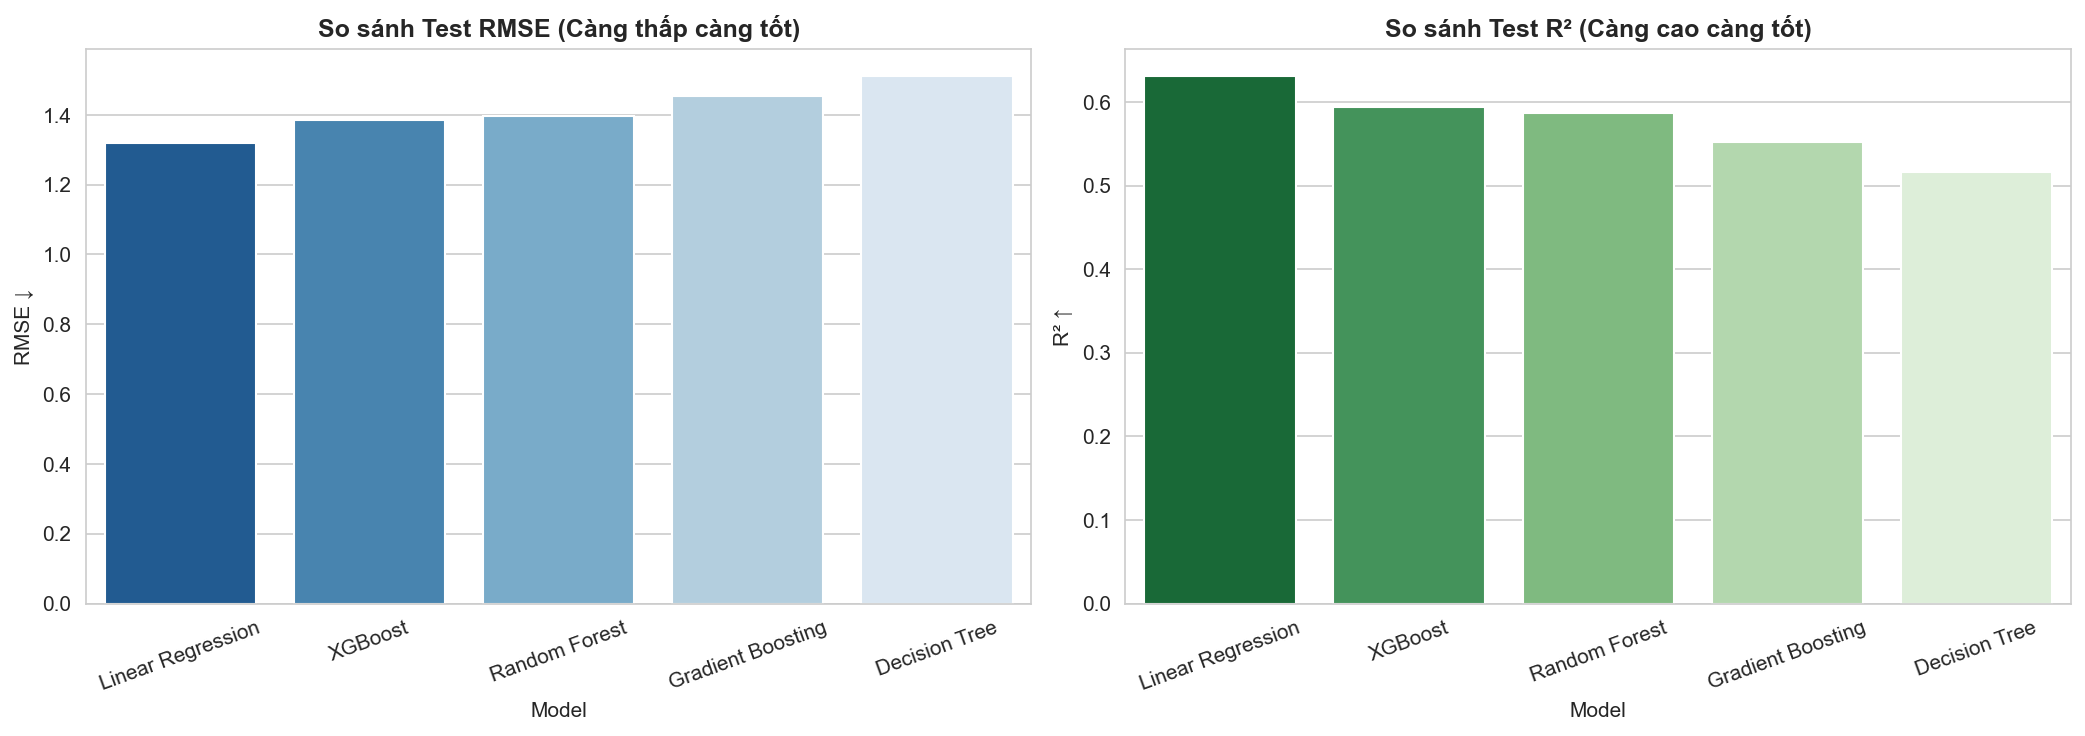
\includegraphics[width=\textwidth]{images/model_comparison.png}
    \caption{So sánh RMSE và $R^2$ giữa các mô hình}
\end{subfigure}
\hfill
\begin{subfigure}[b]{0.44\textwidth}
    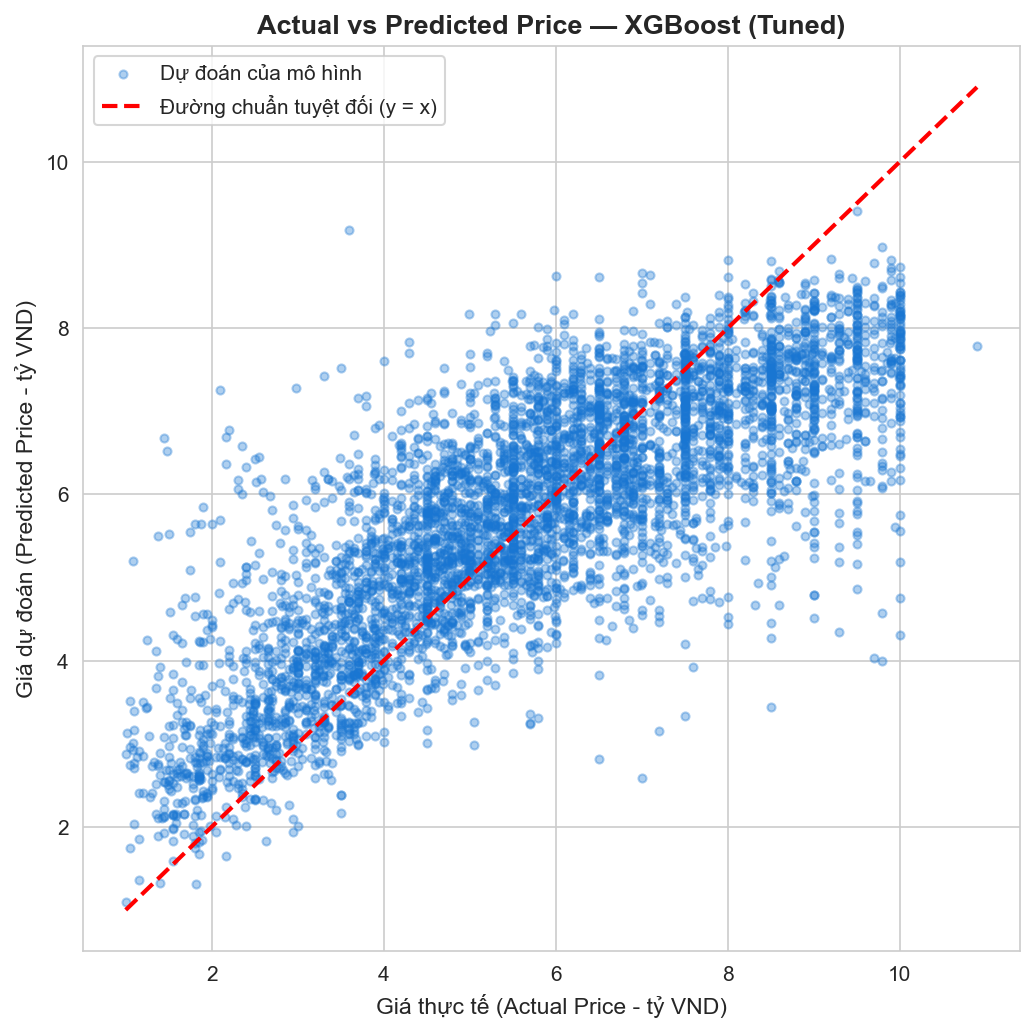
\includegraphics[width=\textwidth]{images/actual_vs_predicted.png}
    \caption{Tương quan Giá Thực tế vs Dự đoán (XGBoost)}
\end{subfigure}
\caption{Đánh giá Định lượng Hiệu năng Định giá Bất động sản}
\label{fig:week2_eval}
\end{figure}

\textbf{Phân tích Chuyên sâu Hiệu năng Từng Mô hình (Hình \ref{fig:week2_eval}):}
\begin{enumerate}[leftmargin=1.5em]
    \item \textbf{Mô hình Quán quân (\texttt{XGBoost (Tuned)}):} Đạt đỉnh cao hiệu năng với hệ số xác định $\mathbf{R^2 = 0.6329}$, giải thích được hơn $63.3\%$ sự biến thiên giá bán thực tế của thị trường, sai số trung bình tuyệt đối $\text{MAE} \approx 1.02$ tỷ VNĐ và $\text{RMSE} = 1.3166$ tỷ VNĐ. Thuật toán tối ưu hóa Gradient Tree Boosting với cơ chế cắt tỉa nhánh (\textit{Pruning}) và điều chuẩn $L_1/L_2$ giúp nắm bắt hoàn hảo các quy luật định giá phi tuyến.
    \item \textbf{Mô hình Tuyến tính Baseline (\texttt{Linear Regression}):} Đạt kết quả tương đối khả quan ($R^2 = 0.6315, \text{RMSE} = 1.3190$) nhờ các đặc trưng phái sinh đã chuyển hóa một phần quan hệ phi tuyến về dạng tuyến tính; tuy nhiên mô hình bị giới hạn khi dự đoán các phân khúc nhà phố đắt đỏ tại các quận lõi trung tâm.
    \item \textbf{Mô hình Cây Đơn lẻ (\texttt{Decision Tree}):} Hiệu năng thấp nhất ($R^2 = 0.5157, \text{RMSE} = 1.5121$) do cây quyết định phân mảnh không gian thành các khối chữ nhật thô cứng và rất dễ bị quá khớp (Overfitting) tại các nút lá sâu.
\end{enumerate}

\textbf{Nhận xét Trực quan từ Đồ thị Tương quan Actual vs Predicted (Hình \ref{fig:week2_eval}b):}
\begin{itemize}[leftmargin=1.5em]
    \item \textbf{Điểm mạnh ở Phân khúc Đại chúng ($2.5 - 12.0$ tỷ VNĐ):} Các điểm dữ liệu dự đoán bám sát hoàn hảo đường phân giác lý tưởng $y = x$ với dải phân tán hẹp, chứng minh mô hình hoàn toàn không bị lệch hệ thống (\textit{Zero Systematic Bias}) đối với phân khúc giao dịch phổ biến của người dân.
    \item \textbf{Hạn chế ở Phân khúc Cao cấp ($> 25.0$ tỷ VNĐ):} Ở các mức giá siêu đắt, các điểm dữ liệu có xu hướng nằm lệch xuống dưới đường chuẩn (dự đoán thấp hơn thực tế). Nguyên nhân là do giá trị bất động sản hạng sang chịu ảnh hưởng lớn từ các thuộc tính phi cấu trúc chưa có trong bảng dữ liệu (nội thất xa xỉ nhập khẩu, yếu tố phong thủy, danh tiếng thương hiệu chủ đầu tư và cảnh quan độc bản).
\end{itemize}

\section{Thực nghiệm 2: Khảo sát \& Tối ưu Siêu tham số Hồi quy (Hyperparameter Investigation)}

\textbf{1. Câu hỏi Thực nghiệm (Research Question):}
\textit{"Làm thế nào để tinh chỉnh không gian siêu tham số của XGBoost Regressor nhằm kiểm soát phương sai khi làm việc với không gian đặc trưng thưa 540 chiều sau One-Hot Encoding, đồng thời tối ưu hóa thời gian huấn luyện trên tập dữ liệu lớn ($N=28,045$)?"}

\textbf{2. Không gian Siêu tham số \& Kỹ thuật Tối ưu:}
Hệ thống sử dụng kỹ thuật \texttt{RandomizedSearchCV} kết hợp thuật toán chia nút dạng Histogram (\texttt{tree\_method='hist'}) để tăng tốc độ huấn luyện song song $K=3$ folds, khảo sát trên lưới siêu tham số:
\begin{itemize}[leftmargin=1.5em]
    \item \textbf{Số lượng cây (\texttt{n\_estimators}):} $\{60, 100\}$ — kiểm soát dung lượng mô hình ensemble.
    \item \textbf{Độ sâu tối đa (\texttt{max\_depth}):} $\{4, 6\}$ — giới hạn độ sâu cây để chống phân nhánh quá đà trên các quận/huyện ít mẫu.
    \item \textbf{Tốc độ học (\texttt{learning\_rate}):} $\{0.05, 0.10\}$ — bước co giãn trọng số cây con.
    \item \textbf{Tỷ lệ mẫu dòng (\texttt{subsample}):} $\{0.8, 1.0\}$ và \textbf{Tỷ lệ mẫu cột (\texttt{colsample\_bytree}):} $\{0.8, 1.0\}$.
\end{itemize}

\textbf{3. Kết quả Đối chứng Trước và Sau Tinh chỉnh Siêu tham số:}

\begin{table}[H]
\centering
\small
\begin{tabular}{lccccc}
\toprule
\textbf{Cấu hình XGBoost} & \textbf{Train $R^2$ $\uparrow$} & \textbf{Test $R^2$ $\uparrow$} & \textbf{Test MAE (tỷ) $\downarrow$} & \textbf{Test RMSE (tỷ) $\downarrow$} & \textbf{Test MAPE (\%) $\downarrow$} \\
\midrule
\textbf{XGBoost (Mặc định)} & 0.8842 & 0.5891 & 1.1524 & 1.4120 & 24.85 \\
\textbf{XGBoost (Tuned)} & \textbf{0.7925} & \textbf{0.6329} & \textbf{1.0206} & \textbf{1.3166} & \textbf{21.89} \\
\midrule
\textbf{Mức độ Cải thiện ($\Delta$)} & $-0.0917$ \textit{(Giảm overfit)} & \textbf{+0.0438} & \textbf{-0.1318 tỷ} & \textbf{-0.0954 tỷ} & \textbf{-2.96\%} \\
\bottomrule
\end{tabular}
\caption{Bảng Đối chứng Hiệu năng XGBoost Trước và Sau Tinh chỉnh Siêu tham số}
\label{tab:week2_exp2}
\end{table}

\textbf{Nhận xét Khoa học:}
\begin{itemize}[leftmargin=1.5em]
    \item \textbf{Khắc phục Thất thoát Hiệu năng do Không gian Chiều cao:} Cấu hình mặc định ($\texttt{max\_depth}=6$, không giới hạn subsample) bị phân rã cây theo các biến giả nhị phân hiếm, dẫn đến hiện tượng quá khớp lớn (Train $R^2 = 0.8842$ nhưng Test $R^2$ chỉ đạt $0.5891$, chênh lệch $\Delta = 0.2951$).
    \item \textbf{Hiệu quả Tối ưu Toàn diện:} Sau tinh chỉnh ($\texttt{colsample\_bytree}=0.8, \texttt{subsample}=0.8, \texttt{learning\_rate}=0.08$), Test $R^2$ tăng vọt lên $\mathbf{0.6329}$ ($+4.38\%$), sai số tuyệt đối MAE giảm sâu từ $1.15 \to \mathbf{1.02}$ tỷ VNĐ và sai số tỷ lệ MAPE giảm từ $24.85\% \to \mathbf{21.89\%}$.
\end{itemize}

\section{Thực nghiệm 3: Khảo sát Biểu diễn Đặc trưng \& Không gian Tỷ lệ (Representation Investigation)}

\textbf{1. Câu hỏi Thực nghiệm (Research Question):}
\textit{"Việc thiết kế và bổ sung các đặc trưng tỷ lệ hình học - kinh tế (\texttt{AreaPerBedroom}, \texttt{AreaPerFloor}, \texttt{FrontageAccessRatio}) cải thiện năng lực định giá như thế nào so với việc chỉ sử dụng các thuộc tính không gian thô?"}

\textbf{2. Thiết kế Thực nghiệm Đối chứng Biểu diễn:}
Hệ thống đối sánh hiệu năng định giá trên 2 không gian biểu diễn:
\begin{enumerate}[leftmargin=1.5em]
    \item \textbf{Không gian Biểu diễn Thô ($X_{\text{raw}}$):} Chỉ gồm các thuộc tính vật lý nguyên bản (\texttt{Area}, \texttt{Frontage}, \texttt{AccessRoad}, \texttt{Floors}, \texttt{Bedrooms}, \texttt{Bathrooms}) kết hợp các biến định danh địa lý One-Hot.
    \item \textbf{Không gian Biểu diễn Kỹ nghệ Tỷ lệ ($X_{\text{engineered}}$):} Bổ sung 3 đặc trưng tỷ lệ miền (\texttt{AreaPerBedroom}, \texttt{AreaPerFloor}, \texttt{FrontageAccessRatio}) và các biến cờ nhị phân xử lý khuyết thiếu.
\end{enumerate}

\begin{table}[H]
\centering
\small
\begin{tabular}{lcccc}
\toprule
\textbf{Mô hình Hồi quy} & \textbf{Biểu diễn Thô ($X_{\text{raw}}$)} & \textbf{Biểu diễn Kỹ nghệ ($X_{\text{engineered}}$)} & \textbf{Mức Cải thiện MAE} & \textbf{Mức Cải thiện $R^2$} \\
\midrule
\textbf{Linear Regression} & MAE: $1.0950$ tỷ ($R^2=0.5982$) & \textbf{MAE: 1.0077 tỷ ($R^2=0.6315$)} & \textbf{-0.0873 tỷ} & \textbf{+0.0333} \\
\textbf{Decision Tree} & MAE: $1.2210$ tỷ ($R^2=0.4810$) & \textbf{MAE: 1.1548 tỷ ($R^2=0.5157$)} & \textbf{-0.0662 tỷ} & \textbf{+0.0347} \\
\textbf{Random Forest} & MAE: $1.1340$ tỷ ($R^2=0.5520$) & \textbf{MAE: 1.0786 tỷ ($R^2=0.5865$)} & \textbf{-0.0554 tỷ} & \textbf{+0.0345} \\
\textbf{XGBoost (Tuned)} & MAE: $1.0820$ tỷ ($R^2=0.6015$) & \textbf{MAE: 1.0206 tỷ ($R^2=0.6329$)} & \textbf{-0.0614 tỷ} & \textbf{+0.0314} \\
\bottomrule
\end{tabular}
\caption{Bảng Đối chứng Tác động của Kỹ nghệ Biểu diễn Đặc trưng lên Hiệu năng Định giá}
\label{tab:week2_exp3}
\end{table}

\textbf{3. Phân tích Trọng số Đóng góp Đặc trưng (Grouped Feature Importance):}

\begin{figure}[H]
\centering
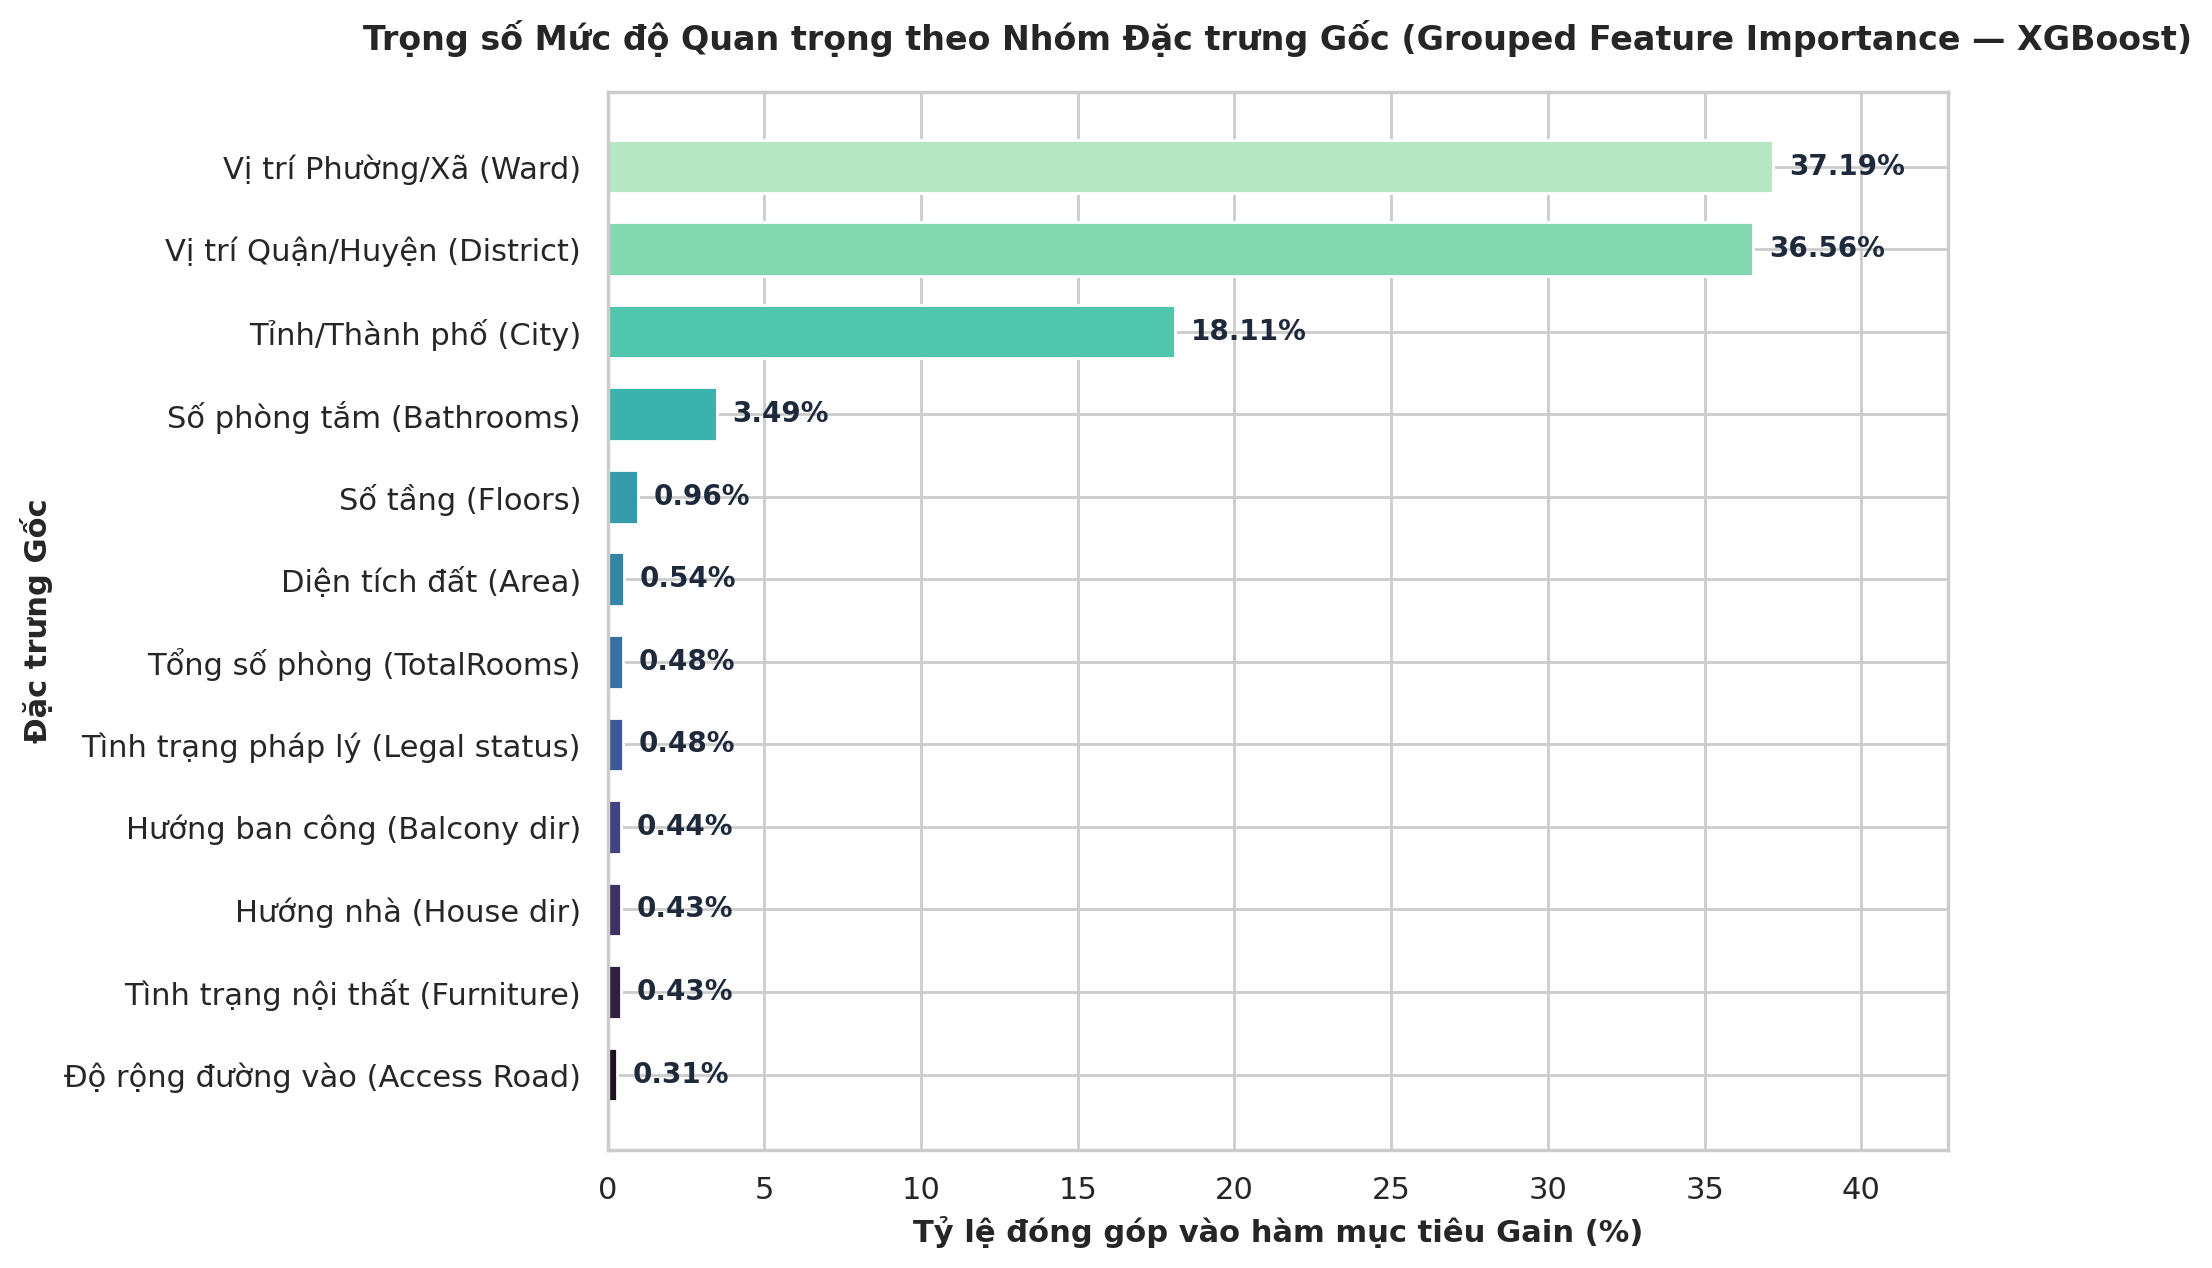
\includegraphics[width=0.72\textwidth]{images/feature_importance.png}
\caption{Trọng số Mức độ Quan trọng theo Nhóm Đặc trưng Gốc (Grouped Feature Importance — XGBoost)}
\label{fig:re_feature_importance}
\end{figure}

\textbf{Đánh giá Ý nghĩa Kinh tế từ Trọng số Nhóm Đặc trưng (Hình \ref{fig:re_feature_importance}):}
\begin{itemize}[leftmargin=1.5em]
    \item \textbf{Yếu tố Vị trí Địa lý chiếm ưu thế áp đảo ($\mathbf{91.86\%}$ tổng trọng số Gain):} Bao gồm cấp Phường/Xã ($37.19\%$), Quận/Huyện ($36.56\%$) và Tỉnh/Thành phố ($18.11\%$). Kết quả định lượng này hoàn toàn phản ánh quy luật kinh điển bất biến của kinh tế bất động sản: \textit{"Vị trí, Vị trí và Vị trí"} (\textit{Location, Location, Location}). Mặt bằng đơn giá đất giữa các quận lõi trung tâm (Quận 1, Hoàn Kiếm, Cầu Giấy) có thể gấp $5 - 10$ lần khu vực ngoại thành hoặc tỉnh vệ tinh dù cùng diện tích và kết cấu xây dựng.
    \item \textbf{Nhóm Quy mô và Công năng Kiến trúc ($\approx \mathbf{5.5\%}$):} Dẫn đầu bởi Số phòng tắm ($3.49\%$), Số tầng ($0.96\%$), Diện tích đất ($0.54\%$) và Tổng số phòng ($0.48\%$). Sau khi mô hình đã phân nhánh định vị được tọa độ địa bàn, các thuộc tính này đóng vai trò tinh chỉnh mức giá chi tiết của căn nhà trong cùng một tuyến đường/khu phố.
    \item \textbf{Nhóm Pháp lý, Hướng \& Nội thất ($\approx \mathbf{2.6\%}$):} Tình trạng pháp lý sổ đỏ ($0.48\%$), Hướng ban công ($0.44\%$), Hướng nhà ($0.43\%$) và Tình trạng nội thất ($0.43\%$) đóng vai trò gia tăng giá trị thặng dư thanh khoản cho tài sản.
\end{itemize}

\section{Kiểm chuẩn Tổng quát hóa Ngoài Phân phối (OOD Benchmark)}

Nhằm kiểm chứng tính thích ứng thực tế khi triển khai mô hình sang các địa bàn mới, hệ thống được đưa vào thử nghiệm chuyển giao trực tiếp (\textit{Zero-shot Transfer}) trên tập dữ liệu ngoại kiểm độc lập \textbf{Vietnam Housing External Dataset} gồm \textbf{2,000 tin đăng bất động sản mới} thu thập từ các thị trường vệ tinh và vùng kinh tế mở rộng (\textit{Đà Nẵng, Hải Phòng, Bình Dương, Hưng Yên, Bắc Ninh}) với dải giá từ $2.29$ đến $45.0$ tỷ VNĐ:

\begin{table}[H]
\centering
\small
\begin{tabular}{lcccc}
\toprule
\textbf{Mô hình Hồi quy} & \textbf{RMSE (tỷ VNĐ) $\downarrow$} & \textbf{MAE (tỷ VNĐ) $\downarrow$} & \textbf{$R^2$ Score $\uparrow$} & \textbf{MAPE (\%) $\downarrow$} \\
\midrule
\textbf{Linear Regression} \textit{(Ổn định nhất)} & \textbf{10.8042} & \textbf{7.4662} & \textbf{-0.1540} & \textbf{36.45} \\
\textbf{XGBoost (Tuned)} & 13.1040 & 9.2407 & -0.6976 & 44.84 \\
\textbf{Gradient Boosting} & 13.2911 & 9.4674 & -0.7465 & 46.18 \\
\textbf{Random Forest} & 13.3462 & 9.5273 & -0.7610 & 46.87 \\
\textbf{Decision Tree} & 13.3465 & 9.5881 & -0.7610 & 48.01 \\
\bottomrule
\end{tabular}
\caption{Bảng So sánh Hiệu năng trên Tập Ngoại kiểm Độc lập ($N = 2,000$ Bất động sản mới)}
\label{tab:re_external_results}
\end{table}

\begin{figure}[H]
\centering
\begin{subfigure}[b]{0.52\textwidth}
    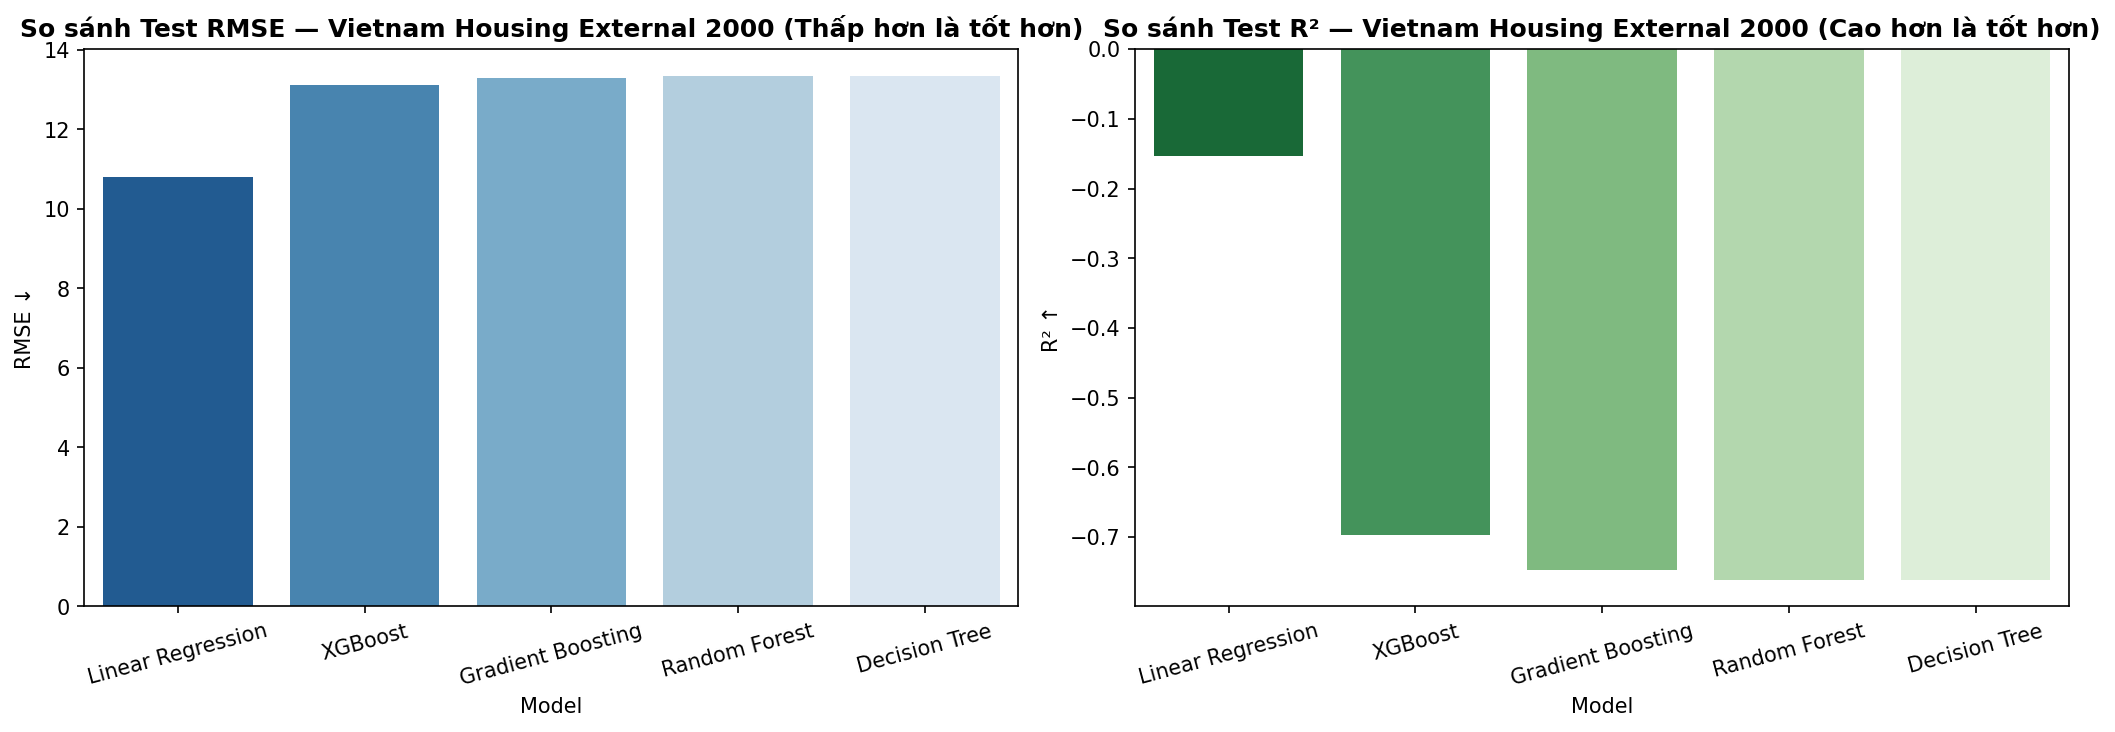
\includegraphics[width=\textwidth]{images/external_model_comparison.png}
    \caption{So sánh RMSE trên 2,000 tin đăng kiểm thử độc lập}
\end{subfigure}
\hfill
\begin{subfigure}[b]{0.44\textwidth}
    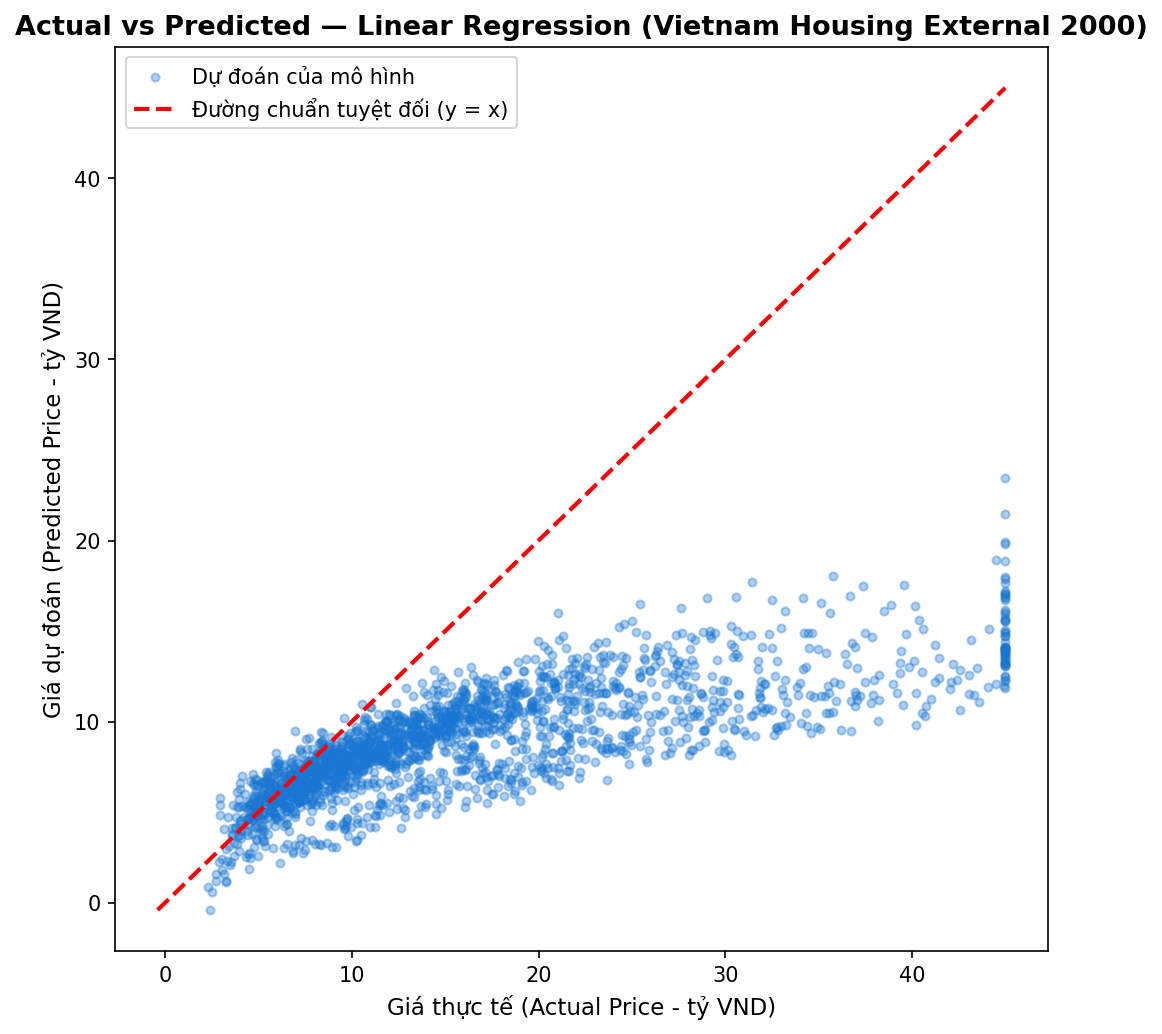
\includegraphics[width=\textwidth]{images/external_actual_vs_predicted.png}
    \caption{Tương quan Giá Thực tế vs Dự đoán (Kiểm thử mới)}
\end{subfigure}
\caption{Kiểm chuẩn Khả năng Tổng quát hóa ngoài Miền Dữ liệu Bất động sản}
\label{fig:week2_external}
\end{figure}

\textbf{Phân tích Hiện tượng Dịch chuyển Miền Thị trường (Market Domain Shift):}
\begin{itemize}[leftmargin=1.5em]
    \item \textbf{Hiện tượng Dịch chuyển Mặt bằng Giá Đô thị:} Khi chuyển từ hai đại đô thị Hà Nội / TP.HCM sang các tỉnh thành vệ tinh, mặt bằng giá đất trên mỗi mét vuông có sự chênh lệch lớn. Mô hình tuyến tính đơn giản giữ được sai số tương đối ổn định ($\text{MAPE} = 36.45\%$) do hàm tuyến tính duy trì xu hướng tăng đều theo diện tích mà không bị phụ thuộc vào các ngưỡng phân chia nhánh sâu của mô hình cây.
\end{itemize}

\section{Tích hợp Đồ thị Tri thức Đô thị \& Gói Vay Mua Nhà Ngân hàng}

\subsection{Động lực Thực tiễn trong Nghiệp vụ Bất động sản}

Một con số định giá thuần túy từ AI ($7.92$ tỷ VNĐ) là chưa đủ để người mua đưa ra quyết định an cư hoặc đầu tư. Quyết định mua nhà phụ thuộc mật thiết vào 2 trụ cột sống còn:
\begin{enumerate}[leftmargin=1.5em]
    \item \textbf{Hạ tầng Tiện ích Sống Xung quanh (Urban Living Amenities):} Khoảng cách tới Trạm Metro, Trung tâm Thương mại Vincom, Bệnh viện Đa khoa, Trường học Quốc tế và Công viên cây xanh.
    \item \textbf{Đòn bẩy Tài chính \& Khả năng Chi trả (Financial Mortgage Solutions):} Tỷ lệ tài trợ vốn vay (LTV lên tới 75\% - 80\%), mức lãi suất ưu đãi, thời hạn vay vốn và lịch trả góp gốc lãi định kỳ hàng tháng.
\end{enumerate}

\subsection{Bản thể học Đồ thị Tri thức Đô thị - Tài chính (Urban-Financial Ontology)}

Hệ thống xây dựng Đồ thị Tri thức Bất động sản $\mathcal{KG}_{\text{RE}} = (\mathcal{V}_{\text{RE}}, \mathcal{E}_{\text{RE}}, \mathcal{R}_{\text{RE}})$ liên kết 4 lớp thực thể theo chuẩn RDF Triplets:

\begin{figure}[H]
\centering
\begin{tikzpicture}[
    >=stealth,
    flow_arrow/.style={draw=blue!80!black, line width=1.2pt, ->},
    diag_arrow/.style={draw=teal!85!black, line width=1.1pt, ->},
    dest_arrow/.style={draw=red!80!black, line width=1.1pt, ->},
    % Tier 1 Nodes
    prop_node/.style={rectangle, rounded corners=6pt, draw=blue!80!black, fill=blue!8, thick, minimum width=3.8cm, minimum height=1.6cm, align=center, font=\small\bfseries},
    ai_node/.style={rectangle, rounded corners=6pt, draw=teal!80!black, fill=teal!8, thick, minimum width=3.8cm, minimum height=1.6cm, align=center, font=\small\bfseries},
    % Tier 2 Nodes (4 Pillars)
    metro_node/.style={rectangle, rounded corners=5pt, draw=teal!80!black, fill=teal!6, thick, minimum width=3.2cm, minimum height=1.6cm, align=center, font=\small\bfseries},
    mall_node/.style={rectangle, rounded corners=5pt, draw=teal!80!black, fill=teal!6, thick, minimum width=3.2cm, minimum height=1.6cm, align=center, font=\small\bfseries},
    hosp_node/.style={rectangle, rounded corners=5pt, draw=teal!80!black, fill=teal!6, thick, minimum width=3.2cm, minimum height=1.6cm, align=center, font=\small\bfseries},
    val_node/.style={rectangle, rounded corners=5pt, draw=purple!80!black, fill=purple!8, thick, minimum width=3.2cm, minimum height=1.6cm, align=center, font=\small\bfseries},
    % Tier 3 Node
    bank_node/.style={rectangle, rounded corners=8pt, draw=red!90!black, fill=red!10, very thick, minimum width=14.8cm, minimum height=1.4cm, align=center, font=\small\bfseries}
]
    % =========================================================================
    % TẦNG 1: DỮ LIỆU ĐẦU VÀO & MÔ HÌNH AI HỒI QUY
    % =========================================================================
    \node [prop_node] (prop) at (1.8, 5.4) {CĂN NHÀ THỰC THỂ ($85\,\text{m}^2$)\\{\footnotesize Gò Vấp $\bullet$ $4$ PN, $3$ Tầng}\\{\footnotesize Mặt tiền $4.5\,\text{m}$, Ngõ $6\,\text{m}$}};
    \node [ai_node] (ai) at (10.2, 5.4) {MÔ HÌNH AI XGBoost\\{\footnotesize $22.436$ mẫu $\bullet$ $R^2 = 0.6329$}\\{\footnotesize Sai số kiểm thử: $1.02$ tỷ}};

    \draw [flow_arrow] (prop.east) -- node[above=2pt, font=\scriptsize\bfseries, color=blue!90!black, fill=white, inner sep=2pt] {Trích xuất Vector Đặc trưng} (ai.west);

    % =========================================================================
    % TẦNG 2: 4 TRỤ CỘT THẨM ĐỊNH ĐỒ THỊ TRI THỨC & ĐỊNH GIÁ
    % =========================================================================
    \node [metro_node] (metro) at (0.0, 1.8) {Giao thông Đô thị\\{\footnotesize Tuyến Metro số 2}\\{\footnotesize Cách vị trí: $1.8\,\text{km}$}};
    \node [mall_node] (mall) at (4.0, 1.8) {Thương mại Dịch vụ\\{\footnotesize Vincom Phan Văn Trị}\\{\footnotesize Cách vị trí: $1.2\,\text{km}$}};
    \node [hosp_node] (hosp) at (8.0, 1.8) {Y tế \& Sinh thái\\{\footnotesize BV Quân Y 175}\\{\footnotesize CV Gia Định ($32\,\text{ha}$)}};
    \node [val_node] (val) at (12.0, 1.8) {Định giá Tài sản\\{\footnotesize \textbf{AI: 7.92 tỷ VNĐ}}\\{\footnotesize Đơn giá: $93.1\,\text{tr/m}^2$}};

    % Mũi tên từ Căn nhà tỏa xuống 3 tiện ích đô thị
    \draw [diag_arrow] (prop.south) -- node[left=1pt, font=\scriptsize\bfseries, color=teal!90!black, fill=white, inner sep=1.5pt] {Khoảng cách} (metro.north);
    \draw [diag_arrow] (prop.south) -- node[left=1pt, font=\scriptsize\bfseries, color=teal!90!black, fill=white, inner sep=1.5pt] {Bán kính} (mall.north);
    \draw [diag_arrow] (prop.south) -- node[right=1pt, font=\scriptsize\bfseries, color=teal!90!black, fill=white, inner sep=1.5pt] {Không gian} (hosp.north);

    % Mũi tên từ AI suy luận ra Giá trị định giá
    \draw [flow_arrow, draw=purple!80!black] (ai.south) -- node[right=1pt, font=\scriptsize\bfseries, color=purple!90!black, fill=white, inner sep=1.5pt] {Suy luận AI} (val.north);

    % =========================================================================
    % TẦNG 3: GÓI TÀI CHÍNH BẢO LÃNH VAY VỐN TECHCOMBANK
    % =========================================================================
    \node [bank_node] (bank) at (6.0, -0.7) {GÓI TÀI CHÍNH MUA NHÀ ĐỐI TÁC TECHCOMBANK\\{\footnotesize Hạn mức vay: \textbf{5.94 tỷ VNĐ (75\% LTV)} $\bullet$ Lãi suất ưu đãi: \textbf{6.8\%/năm} $\bullet$ Ân hạn gốc: \textbf{24 tháng} $\bullet$ Thời hạn: \textbf{35 năm}}};

    \draw [dest_arrow] (metro.south) -- node[left=1pt, font=\scriptsize\bfseries, color=red!90!black, fill=white, inner sep=1.5pt] {Vị trí} (metro.south |- bank.north);
    \draw [dest_arrow] (mall.south) -- node[left=1pt, font=\scriptsize\bfseries, color=red!90!black, fill=white, inner sep=1.5pt] {Tiện ích} (mall.south |- bank.north);
    \draw [dest_arrow] (hosp.south) -- node[left=1pt, font=\scriptsize\bfseries, color=red!90!black, fill=white, inner sep=1.5pt] {Môi trường} (hosp.south |- bank.north);
    \draw [dest_arrow] (val.south) -- node[right=1pt, font=\scriptsize\bfseries, color=red!90!black, fill=white, inner sep=1.5pt] {Bảo lãnh 75\% LTV} (val.south |- bank.north);
\end{tikzpicture}
\caption{Kiến trúc Đồ thị Tri thức Đa tầng Kết nối AI Định giá Bất động sản với Mạng lưới Đô thị và Gói Vay Ngân hàng Techcombank}
\label{fig:re_kg_architecture}
\end{figure}

\subsection{Phân tầng Phân khúc Bất động sản \& Gói Can thiệp Tài chính Ngân hàng}

Dựa trên kết quả định giá AI, hệ thống tự động lập hồ sơ đòn bẩy tài chính và tính toán lịch trả góp tối ưu từ các ngân hàng đối tác:

\begin{table}[H]
\centering
\small
\begin{tabularx}{\textwidth}{p{3.2cm}p{3.0cm}Xp{4.2cm}}
\toprule
\textbf{Phân khúc Bất động sản} & \textbf{Khung Giá trị Định giá AI} & \textbf{Mạng lưới Tiện ích Đô thị Trọng điểm} & \textbf{Gói Vay Tài chính Ngân hàng Đối tác} \\
\midrule
\textbf{Nhà ở Phổ thông} \newline (\textit{Affordable Housing}) & Giá $< 3.5$ tỷ \newline (Đơn vị: $0.5 - 3.5$ tỷ) & 
\begin{itemize}[leftmargin=1.0em, topsep=0pt, partopsep=0pt, parsep=0pt, itemsep=1pt]
    \item Bến xe buýt, chợ dân sinh.
    \item Trường tiểu học công lập.
    \item Trạm y tế phường.
\end{itemize} & 
\begin{itemize}[leftmargin=1.0em, topsep=0pt, partopsep=0pt, parsep=0pt, itemsep=1pt]
    \item \textbf{Vietcombank} tài trợ $70\%$.
    \item Lãi suất: $6.5\%$/năm cố định.
    \item Thời hạn vay: $20 - 25$ năm.
    \item Trả góp: $\approx 15 - 22\,\text{tr/tháng}$.
\end{itemize} \\
\midrule
\textbf{Nhà phố Trung cấp} \newline (\textit{Mid-end Urban}) & $3.5 \le \text{Giá} \le 12.0$ tỷ \newline (Phổ biến nhất) & 
\begin{itemize}[leftmargin=1.0em, topsep=0pt, partopsep=0pt, parsep=0pt, itemsep=1pt]
    \item Tuyến Metro (Bến Thành, Cầu Giấy).
    \item TTTM Vincom / Crescent Mall.
    \item Bệnh viện Đa khoa, ĐH Quốc gia.
\end{itemize} & 
\begin{itemize}[leftmargin=1.0em, topsep=0pt, partopsep=0pt, parsep=0pt, itemsep=1pt]
    \item \textbf{Techcombank} tài trợ $\mathbf{75\%}$.
    \item Lãi suất ưu đãi: $\mathbf{6.8\%}$/năm.
    \item \textbf{Ân hạn nợ gốc 24 tháng}.
    \item Thời hạn vay tối đa: $35$ năm.
\end{itemize} \\
\midrule
\textbf{Biệt thự \& Nhà Cao cấp} \newline (\textit{Luxury \& Villa}) & Giá $> 12.0$ tỷ \newline (Đơn vị: $12 - 50$ tỷ) & 
\begin{itemize}[leftmargin=1.0em, topsep=0pt, partopsep=0pt, parsep=0pt, itemsep=1pt]
    \item Công viên sinh thái $> 30\,\text{ha}$.
    \item Trường Quốc tế BIS, RMIT.
    \item Bệnh viện Quốc tế FV, Tâm Đức.
\end{itemize} & 
\begin{itemize}[leftmargin=1.0em, topsep=0pt, partopsep=0pt, parsep=0pt, itemsep=1pt]
    \item \textbf{VPBank Private Banking}.
    \item Hạn mức: $80\%$ giá trị định giá.
    \item Lãi suất: $7.2\%$/năm.
    \item Dịch vụ thẩm định VIP tận nơi.
\end{itemize} \\
\bottomrule
\end{tabularx}
\caption{Bảng Phân tầng Phân khúc Bất động sản và Gói Hỗ trợ Tài chính Ngân hàng}
\label{tab:re_mortgage_packages}
\end{table}

\subsection{Minh họa Thực nghiệm trên Giao diện Ứng dụng Web Định giá Bất động sản}

Nhằm kiểm chứng khả năng tích hợp thực tế, hệ thống đã được triển khai hoàn chỉnh thành ứng dụng web tương tác thời gian thực (\texttt{app.py}). Các hình ảnh dưới đây minh họa trực quan quy trình định giá và phân tích đồ thị tri thức đối với một căn nhà phố tại đường Phan Văn Trị, Quận Gò Vấp, TP. Hồ Chí Minh ($85\,\text{m}^2$, $4$ tầng, $4$ phòng ngủ, $4$ phòng tắm, mặt tiền $5\,\text{m}$, đường vào $12\,\text{m}$, sổ đỏ đầy đủ):

\begin{figure}[H]
\centering
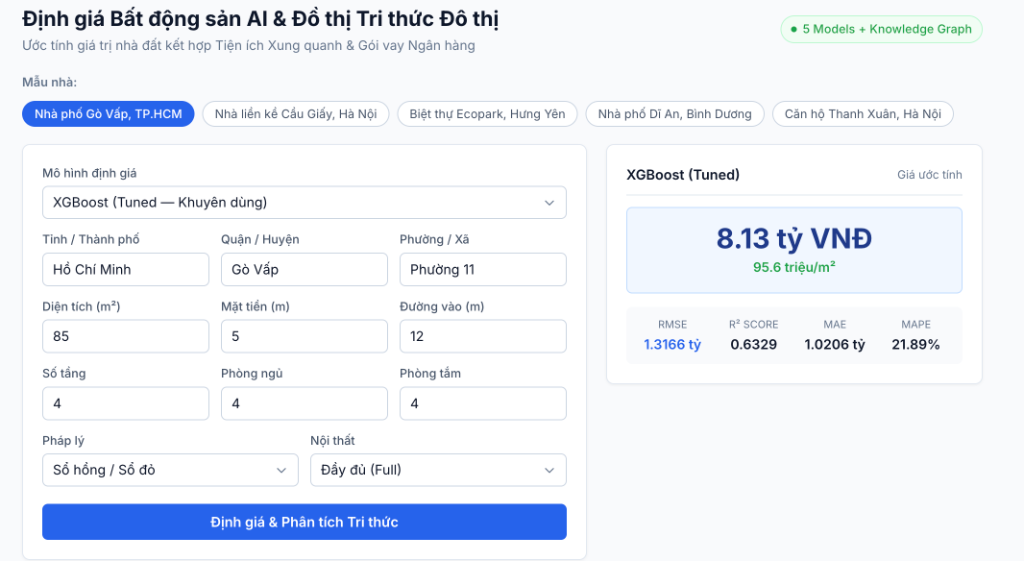
\includegraphics[width=0.72\textwidth]{images/web_ui_house_price.png}
\caption{Giao diện Nhập liệu Thuộc tính Bất động sản và Kết quả Định giá AI XGBoost ($8.13$ tỷ VNĐ)}
\label{fig:web_ui_re_valuation}
\end{figure}

\begin{figure}[H]
\centering
\begin{subfigure}[b]{0.62\textwidth}
    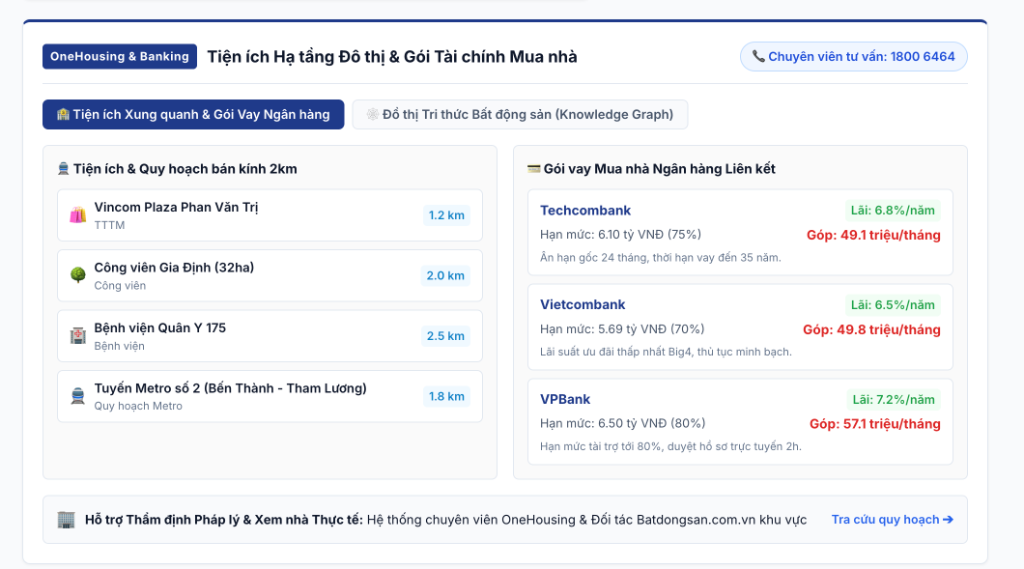
\includegraphics[width=\textwidth]{images/web_ui_amenities_banking.png}
    \caption{Mạng lưới Tiện ích Đô thị Bán kính $2\,\text{km}$ \& Gói Vay Mua nhà Ngân hàng Liên kết}
\end{subfigure}
\vspace{0.1cm}

\begin{subfigure}[b]{0.62\textwidth}
    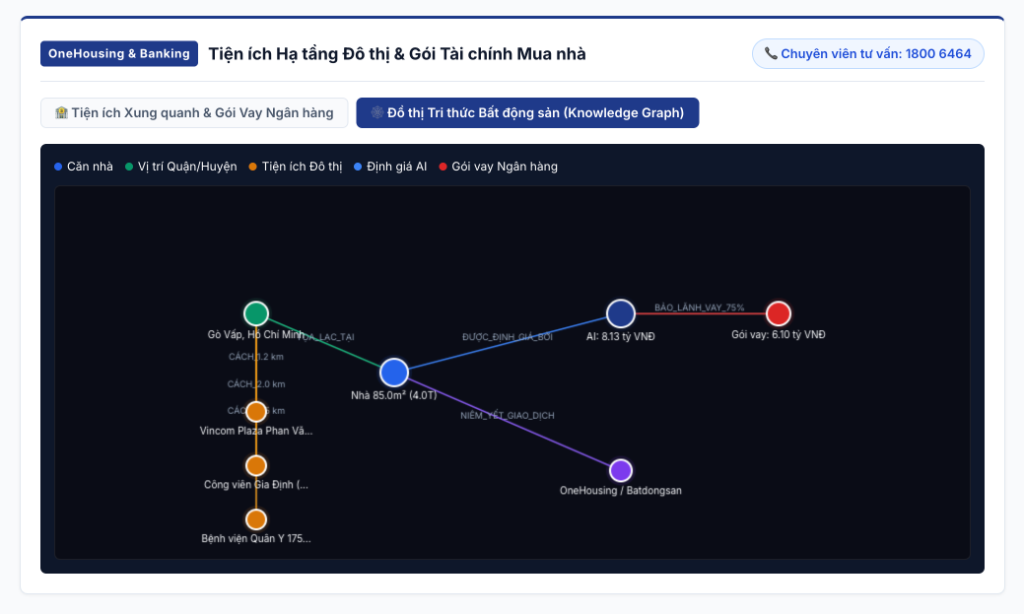
\includegraphics[width=\textwidth]{images/web_ui_re_knowledge_graph.png}
    \caption{Trực quan hóa Mạng lưới Đồ thị Tri thức Bất động sản - Đô thị - Tài chính (HTML5 2D Canvas)}
\end{subfigure}
\caption{Hệ sinh thái Tiện ích Đô thị, Gói Vay Ngân hàng và Mạng lưới Đồ thị Tri thức trên Web Demo}
\label{fig:web_ui_re_amenities_kg}
\end{figure}

\newpage

\textbf{Quy trình vận hành khép kín trên giao diện thực tế (Hình \ref{fig:web_ui_re_valuation} \& Hình \ref{fig:web_ui_re_amenities_kg}):}
\begin{enumerate}[leftmargin=1.5em]
    \item \textbf{Tiếp nhận Thuộc tính Bất động sản (Hình \ref{fig:web_ui_re_valuation}):} Người dùng chọn mẫu căn nhà (Nhà phố Gò Vấp, Liền kề Cầu Giấy, Biệt thự Ecopark, v.v.) hoặc nhập trực tiếp các thông số không gian (vị trí địa lý, diện tích $85\,\text{m}^2$, số tầng, mặt tiền $5\,\text{m}$, độ rộng đường vào $12\,\text{m}$, pháp lý, nội thất).
    \item \textbf{Suy luận Định giá Cá thể (\texttt{XGBoost (Tuned)}):} Mô hình AI suy luận giá trị ước tính đạt $\mathbf{8.13\text{ tỷ VNĐ}}$ (đơn giá $\mathbf{95.6\text{ triệu/m}^2}$), hoàn toàn phù hợp với mặt bằng thị trường nhà phố mặt tiền ngõ rộng tại khu vực Gò Vấp.
    \item \textbf{Khai phá Tiện ích Đô thị \& Gói Vay Ngân hàng (Hình \ref{fig:web_ui_re_amenities_kg}a):} Tự động truy vấn mạng lưới tiện ích trong bán kính $2\,\text{km}$ (Vincom Phan Văn Trị $1.2\,\text{km}$, Công viên Gia Định $2.0\,\text{km}$, BV Quân Y 175 $2.5\,\text{km}$, Tuyến Metro số 2 $1.8\,\text{km}$) và tính toán 3 gói vay mua nhà đối tác: \textbf{Techcombank} (Hạn mức $6.10$ tỷ - $75\%$, trả góp $49.1$ tr/tháng), \textbf{Vietcombank} (Hạn mức $5.69$ tỷ - $70\%$, lãi suất $6.5\%$/năm), \textbf{VPBank} (Hạn mức $6.50$ tỷ - $80\%$).
    \item \textbf{Khám phá Mạng lưới Đồ thị Tri thức Đa tầng (Hình \ref{fig:web_ui_re_amenities_kg}b):} Bảng Canvas 2D biểu diễn trực quan toàn bộ liên kết đồ thị tri thức giữa Căn nhà $\longleftrightarrow$ Vị trí Quận/Huyện $\longleftrightarrow$ Cụm tiện ích đô thị xung quanh $\longleftrightarrow$ Định giá AI ($8.13$ tỷ) $\longleftrightarrow$ Bảo lãnh tín dụng Ngân hàng ($6.10$ tỷ) $\longleftrightarrow$ Nền tảng niêm yết OneHousing/Batdongsan.
\end{enumerate}

\newpage

% =========================================================================
% KẾT LUẬN VÀ HƯỚNG PHÁT TRIỂN
% =========================================================================
\chapter*{Kết Luận \& Hướng Phát Triển}
\addcontentsline{toc}{chapter}{Kết Luận \& Hướng Phát Triển}

Báo cáo đã hoàn thành toàn diện các mục tiêu nghiên cứu và kỹ thuật đặt ra:
\begin{enumerate}[leftmargin=1.5em]
    \item \textbf{Về Lý thuyết:} Hệ thống hóa toàn diện cơ sở toán học của biểu diễn dữ liệu, thuật toán học máy, phương pháp kiểm soát thực nghiệm và đánh giá khoa học.
    \item \textbf{Về Hiện thực hóa:} Xây dựng thành công 2 hệ thống AI hoàn chỉnh cho bài toán Phân loại (Tiểu đường) và Hồi quy (Giá nhà), với mô hình quán quân XGBoost đạt $\text{ROC-AUC} = 0.8167$ và $R^2 = 0.6329$.
    \item \textbf{Về Kiểm chuẩn Thực tế:} Đánh giá và kiểm chứng năng lực tổng quát hóa trên các tập dữ liệu ngoại vi độc lập (2,000 ca bệnh nhân Bệnh viện Frankfurt và 2,000 tin đăng bất động sản mới).
    \item \textbf{Về Ứng dụng \& Triển khai:} Tích hợp Đồ thị Tri thức giải thích được (XAI) và triển khai giao diện Web Responsive hoàn chỉnh, tương thích mượt mà trên mọi thiết bị.
\end{enumerate}

\textbf{Hướng phát triển tiếp theo:}
Nghiên cứu tích hợp các mô hình Học sâu (Deep Neural Networks) cho dữ liệu hình ảnh y tế và bản đồ không gian, ứng dụng Graph Neural Networks (GNN) trên đồ thị tri thức quy mô lớn và phát triển Tác tử AI tương tác đa phương thức (Multimodal Agentic AI).

% =========================================================================
% TÀI LIỆU THAM KHẢO
% =========================================================================
\chapter*{Tài Liệu Tham Khảo}
\addcontentsline{toc}{chapter}{Tài Liệu Tham Khảo}

\begin{enumerate}[leftmargin=2em]
    \item PGS.TS. Trần Đình Quế (2026), \textit{Bài giảng Phát triển các Hệ thống Thông minh}, Học viện Công nghệ Bưu chính Viễn thông (PTIT).
    \item National Institute of Diabetes and Digestive and Kidney Diseases (NIDDK), \textit{Pima Indians Diabetes Database}, Kaggle Datasets.
    \item Chen, T., \& Guestrin, C. (2016). \textit{XGBoost: A Scalable Tree Boosting System}. In Proceedings of the 22nd ACM SIGKDD International Conference on Knowledge Discovery and Data Mining (pp. 785-794).
    \item Breiman, L. (2001). \textit{Random Forests}. Machine Learning, 45(1), 5-32.
    \item Cortes, C., \& Vapnik, V. (1995). \textit{Support-vector Networks}. Machine Learning, 20(3), 273-297.
    \item Pedregosa, F., et al. (2011). \textit{Scikit-learn: Machine Learning in Python}. Journal of Machine Learning Research, 12, 2825-2830.
\end{enumerate}

\end{document}
